\documentclass[12pt,a4paper,parskip,bibliography=totoc]{scrbook}
\usepackage{mystyle}

% faster tikz. Needs to be here because of overleaf
\usepgfplotslibrary{external}
\tikzexternalize[prefix=tikzexternalize/]
\makeatletter
\renewcommand{\todo}[2][]{\tikzexternaldisable\@todo[#1]{#2}\tikzexternalenable}
\makeatother


\title{Anwendung von Contraction Hierarchies und Hierarchical Hub-Labeling auf Geometrischen Graphen}
\author{Christian Staib}
\date{\today}

\setcounter{tocdepth}{1}

\begin{document}



\tikzexternaldisable
\begin{titlepage}
    \begin{tikzpicture}[overlay,remember picture,y=-1cm]
        % set a new origin [1]
        \coordinate (O) at (current page.north west);

        \node[text width=9cm,align=flush center,zeilenabstand=1.5] at ($(O)+(10.95,12.05)$)
        {
        {\large Bachelorarbeit}
        \\[0.75\baselineskip]
        {\Large \bfseries \MyTitle}
        \\[0.75\baselineskip]
        {\large \MyAuthor}
        };



        \node[text width=9cm,align=flush center] at ($(O)+(10.95,4.21)$)
        {
            Institut für Formale Methoden der Informatik
            \\[1.5\baselineskip]
            Universität Stuttgart\\
            Universitätsstraße 38\\
            70569 Stuttgart
        };


        \node[] at ($(O)+(10.95,1.75)$)
        {\includegraphics{img/unistuttgart_logo_deutsch.pdf} };


        \node[align=center] at ($(O)+(10.95,24.16)$)
        {
            \begin{tabular}{lll}
                \textbf{Studiengang:} &  & Informatik             \\
                \\
                \textbf{Prüfer}:      &  & Prof. Dr. Stefan Funke \\
                \textbf{Betreuer}:    &  & Daniel Koch            \\
                \\
                \textbf{Beginn am:}   &  & 8. April 2024          \\
                \textbf{Beendet am:}  &  & 8. Oktober 2024        \\
            \end{tabular}
        };
    \end{tikzpicture}

\end{titlepage}
\tikzexternalenable
\cleardoublepage

\chapter{Kurzfassung}

Während Contraction Hierarchies (CH) auf Straßengraphen erfolgreich eingesetzt werden und hohe Speedups bei der Berechnung von kürzesten Pfaden ermöglichen, ist ihre Anwendung auf große Sichtbarkeitsgraphen in angemessener Zeit nicht möglich.
Da bisher keine Contraction Hierarchies für die bearbeiteten Sichtbarkeitsgraphen erstellt werden konnten, war auch die Erzeugung von Hierarchical Hub Labelings (HHL) nicht realisierbar.

Diese Arbeit untersucht die Hindernisse bei der Anwendung von Contraction Hierarchies auf Sichtbarkeitsgraphen und prüft, ob sich die Kontraktion durch den Einsatz von Heuristiken anstelle der Witness-Suche beschleunigen lässt.
Trotz der Anwendung dieser Heuristiken konnten die Sichtbarkeitsgraphen nicht kontrahiert werden.

Basierend auf bestehenden Charakterisierungen werden mit PEOPLE und CH-PEOPLE (\textbf{P}r\textbf{E}determined \textbf{O}rder, \textbf{P}runed \textbf{L}ab\textbf{e}l) zwei Algorithmen vorgestellt, die es ermöglichen, ohne Kontraktion sowohl Hierarchical Hub Labelings als auch die für CH-Anfragen benötigte Datenstruktur zu erstellen.
Beide Algorithmen sind trivial parallelisierbar und wurden erfolgreich auf die bearbeiteten Sichtbarkeitsgraphen angewendet.
Während CH-Anfragen nur einen geringen Speedup erzielten, zeigte sich bei HHL-Anfragen ein deutlicher Performance-Gewinn.
Zudem war die durchschnittliche Labelgröße der Sichtbarkeitsgraphen vergleichbar mit ihrem durchschnittlichen Knotengrad.
\cleardoublepage

\tableofcontents

\cleardoublepage


\mainmatter
\chapter{Einleitung}

Sichtbarkeitsgraphen sind Graphen, die alle Knotenpaare miteinander verbinden, die sich \emph{sehen} können, auf deren \emph{Luftlinie} sich also keine \emph{Hindernisse} befinden.
Aus einer Küstenlinie kann ein Sichtbarkeitsgraph erstellt werden, indem die Knoten auf der Küstenlinie mit allen Knoten verbunden werden, deren Luftlinie keine Küste kreuzt.
\autoref{fig:thessaloniki-visibility} zeigt einen Ausschnitt eines solchen Sichtbarkeitsgraphen.
Zu sehen ist der Hafen der griechischen Stadt Thessaloniki.

Das Finden von kürzesten Pfaden ist in solchen Graphen rechenintensiver als etwa auf Straßengraphen mit vergleichbarer Knotenanzahl, da sie unter anderem einen höheren durchschnittlichen Knotengrad und keine inhärente hierarchische Struktur besitzen.
Zwar gibt es Möglichkeiten, den Graphen zu verändern, und schneller Pfade zwischen Knoten zu berechnen, etwa durch Triangulierung oder Rasterisierung, jedoch sind diese Pfade nicht mehr garantiert optimal.

Im Folgenden wird untersucht, inwiefern sich zwei Techniken zum schnellen Finden von kürzesten Pfaden und kürzesten Pfad-Distanzen (\emph{Contraction Hierarchies} und \emph{Hierarchical Hub Labeling}) auf diese Graphen anwenden lassen.

\begin{figure}[ht]%
  \centering
  \subfloat[\centering aegaeis-visibility]{{\includegraphics[width=.5\linewidth]{img/thessaloniki-visibility.png}}}%
  \caption{Sichtbarkeitsgraph des Hafens von Thessaloniki}%
  \label{fig:thessaloniki-visibility}%
\end{figure}
% 
% 
% 
% 
% \section{Speedup-Techniken}
% 
% Die betrachteten Speedup-Techniken zum Finden kürzester Pfade benötigen eine Phase der Vorbehandlung (\emph{preprocessing}), damit danach kürzeste Pfad Anfragen (\emph{queries}) schneller beantwortet werden können.
% Die für das Preprocessing benutzte Rechenzeit und der Memory-Overhead sollte dabei in einem sinnvollen Verhältnis zum Speedup und der Anzahl der Queries stehen.
% Ist der Speedup besonders hoch, so lohnt es sich mehr in das Preprocessing zu investieren.
% 
% \todo{Speedup Techniken auflisten, Aufwand / Benefit Diagram}
% 
\chapter{Graphen}

Ein Graph ist eine mathematische Struktur zur Darstellung von Beziehungen zwischen Objekten.
Die Idee, Objekte durch Verknüpfungen zu verbinden, bildet die Grundlage für zahlreiche Anwendungen, unter anderem die Routenplanung.
Graphen und insbesondere kürzeste Pfade spielen darüber hinaus eine wichtige Rolle; in einem Wissensgraphen kann ein Pfad etwa die Gültigkeit einer Aussage repräsentieren.
\autoref{graphs:fig:beispielgraph} zeigt einen Graphen, der im Folgenden für Beispiele verwendet wird.

\begin{figure}[ht]
  \centering
  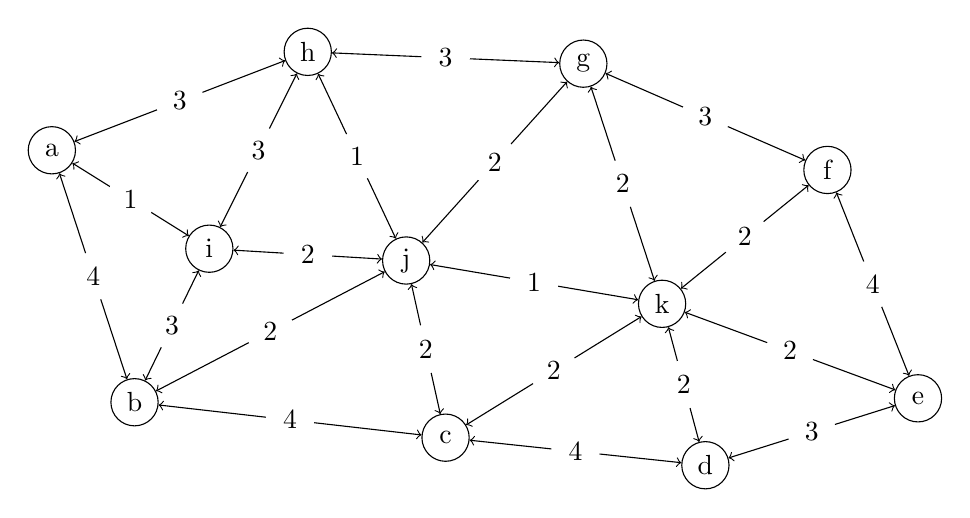
\begin{tikzpicture}
    % Nodes
    \node[circle, draw, minimum size=0.6cm, inner sep=0pt] at (0.5* 0.0, 0.5* 8.5)  (a)    {a};
    \node[circle, draw, minimum size=0.6cm, inner sep=0pt] at (0.5* 2.1, 0.5* 2.1)  (b)    {b};
    \node[circle, draw, minimum size=0.6cm, inner sep=0pt] at (0.5* 10.0, 0.5* 1.2)  (c)    {c};
    \node[circle, draw, minimum size=0.6cm, inner sep=0pt] at (0.5* 16.6, 0.5* 0.5)  (d)    {d};
    \node[circle, draw, minimum size=0.6cm, inner sep=0pt] at (0.5* 22.0, 0.5* 2.2)  (e)    {e};
    \node[circle, draw, minimum size=0.6cm, inner sep=0pt] at (0.5* 19.7, 0.5* 8.0)  (f)    {f};
    \node[circle, draw, minimum size=0.6cm, inner sep=0pt] at (0.5* 13.5, 0.5* 10.7)  (g)    {g};
    \node[circle, draw, minimum size=0.6cm, inner sep=0pt] at (0.5* 6.5, 0.5* 11.0)  (h)    {h};
    \node[circle, draw, minimum size=0.6cm, inner sep=0pt] at (0.5* 4.0, 0.5* 6.0)  (i)    {i};
    \node[circle, draw, minimum size=0.6cm, inner sep=0pt] at (0.5* 9.0, 0.5* 5.7)  (j)    {j};
    \node[circle, draw, minimum size=0.6cm, inner sep=0pt] at (0.5* 15.5, 0.5* 4.6)  (k)    {k};

    \draw[<->]  (a) edge node[circle, fill=white] {4} (b);
    \draw[<->]  (a) edge node[circle, fill=white] {3} (h);
    \draw[<->]  (a) edge node[circle, fill=white] {1} (i);

    \draw[<->]  (b) edge node[circle, fill=white] {4} (c);
    \draw[<->]  (b) edge node[circle, fill=white] {3} (i);
    \draw[<->]  (b) edge node[circle, fill=white] {2} (j);

    \draw[<->]  (c) edge node[circle, fill=white] {4} (d);
    \draw[<->]  (c) edge node[circle, fill=white] {2} (j);
    \draw[<->]  (c) edge node[circle, fill=white] {2} (k);

    \draw[<->]  (d) edge node[circle, fill=white] {3} (e);
    \draw[<->]  (d) edge node[circle, fill=white] {2} (k);

    \draw[<->]  (e) edge node[circle, fill=white] {4} (f);
    \draw[<->]  (e) edge node[circle, fill=white] {2} (k);

    \draw[<->]  (f) edge node[circle, fill=white] {3} (g);
    \draw[<->]  (f) edge node[circle, fill=white] {2} (k);

    \draw[<->]  (g) edge node[circle, fill=white] {3} (h);
    \draw[<->]  (g) edge node[circle, fill=white] {2} (j);
    \draw[<->]  (g) edge node[circle, fill=white] {2} (k);

    \draw[<->]  (h) edge node[circle, fill=white] {3} (i);
    \draw[<->]  (h) edge node[circle, fill=white] {1} (j);

    \draw[<->]  (i) edge node[circle, fill=white] {2} (j);

    \draw[<->]  (j) edge node[circle, fill=white] {1} (k);
  \end{tikzpicture}
  \caption{Graph}
  \label{graphs:fig:beispielgraph}
\end{figure}

\section{Definitionen}
Damit in den nachfolgenden Kapiteln sinnvoll argumentiert werden kann, werden einige grundlegende Begriffe eingeführt.

\begin{definition}[Graph]
  Sofern nicht anders angegeben, bezeichnet Graph im Folgenden einen endlichen, gerichteten Graphen mit Kantengewichten, ohne Mehrfachkanten und Schleifen.

  Als Schreibweise wird $G = (V, E)$ verwendet, wobei $V$ die Knotenmenge und $E$ die Kantenmenge ist. Eine Kante ist hierbei ein Tupel $(t, h, w)$. Man bezeichnet $t \in V$ als \emph{Fuß} (Tail), $h \in V$ als \emph{Kopf} (Head) und $w \in \mathbb{R}^+$ als \emph{Gewicht} (Weight). Gelegentlich wird auch nur $(t, h)$ geschrieben, um auszudrücken, dass zwei Knoten verbunden sind.

  Wird $G$ als ungerichtet bezeichnet, so gilt $(t, h, w) \in E \Leftrightarrow (t, h, w)^T \coloneq (h, t, w) \in E$ und $(t, h)$ kann als $\{ t, h \}$ geschrieben werden.
\end{definition}

Das Gewicht der Kanten ist hierbei auf positive reelle Zahlen begrenzt, da das Verwenden eines Kantengewichtes $0$ dazu führen kann, dass ein kürzester Pfad mehrfach einen Teilpfad der Länge 0 durchläuft.

\begin{definition}[Nachbar]
  Sei $G = (V, E)$. Ein Knoten $u \in V$ heißt \emph{Vorgänger} eines Knotens $v \in V$ wenn $(u, v) \in E$. $v$ ist dann ein \emph{Nachfolger} von $u$.
  Ist $G$ ungerichtet, so spricht man in beiden Fällen von \emph{Nachbarn}.
\end{definition}

Die Anzahl der Nachbarn eines Knotens wird als sein \emph{Grad} bezeichnet, wobei bei gerichteten Graphen vom \emph{Eingangsgrad} und \emph{Ausgangsgrad} gesprochen wird.
Hat ein Knoten keine Vorgänger oder Nachfolger, so nennt man ihn \emph{isoliert}.

\begin{definition}[Pfad]
  Ein Pfad $p$ in einem Graphen $G = (V, E)$ ist eine Folge von Knoten $(v_1, \dotsc, v_n)$, wobei für alle $i \in {1, \dotsc, n-1}$ gilt, dass $(v_i, v_{i+1}) \in E$.
  Der Knoten $v_1$ wird Startknoten, $v_n$ Zielknoten genannt.
  Die Summe der Kantengewichte aller Kanten $(v_i, v_{i + 1})$ wird seine \emph{Länge}, die Anzahl der Kantennutzungen ($n - 1$) seine \emph{Hop-Länge}, genannt.
\end{definition}

Häufig wird für den Startknoten der Buchstabe $s$ (Source) und für den Zielknoten der Buchstabe $t$ (Target) verwendet.
Zwischen zwei Knoten kann es Pfade unterschiedliche Länge geben, dies führt zur Definition des kürzesten Pfades.

\begin{definition}[Kürzester Pfad]
  Ein Pfad $p = (v_1 , \dotsc , v_n)$ ist \emph{ein kürzester Pfad}, wenn die Länge von $p$ unter allen Pfaden von $v_1$ nach $v_n$ minimal ist.
  Die Länge des kürzesten Pfades wird als \emph{Abstand} von $v_1$ und $v_n$ bezeichnet.

  Die Funktion ${spd}_G \colon V \times V \to \mathbb{R}^+_0 \cup \{ \infty \} $ (Shortest Path Distance) weist einem Knotenpaar den Abstand zu, wobei dieser unendlich ist, wenn kein Pfad zwischen ihnen existiert.
  Dann bezeichnet ${sp}_{G} (s, t)$ (Shortest Path) einen kürzesten Pfad zwischen $s$ und $t$.
\end{definition}

Die zu beantwortende Frage, ob es zwischen zwei Knoten $s, t \in V$ einen Pfad gibt und was der Abstand der Knoten ist, bezeichnet man auch als $s$-$t$-Anfrage (Query) und einen gefundenen Pfad als $s$-$t$-Pfad.
Zusätzlich zum Finden eines Pfades zwischen zwei Knoten ist es häufig notwendig, die kürzesten Pfade von einem Knoten zu allen anderen Knoten zu bestimmen.
Auch die Umkehrung dieses Problem ist interessant, also die kürzesten Pfade von allen Knoten zu einem Anderen zu bestimmen.
Diese Probleme sind äquivalent, da das Finden aller kürzesten Pfade zu einem Knoten auf einem Graph $G$ dem Finden aller kürzester Pfade von diesem Knoten auf dem transponierten Graph $G^T$ entspricht.

\begin{definition}[Transponierter Graph]
  Sei $G = (V, E)$ ein Graph. Dann ist $G^T \coloneq (V, E^T)$ mit $(t, h, w) \in E \Leftrightarrow (h, t, w) \in E^T$ der \emph{transponierte Graph} von $G$.
\end{definition}

Ein ungerichteter Graph ist hierbei selbst sein transponierter Graph.

\begin{definition}[Hitting-Set]
  Sei $G = (V, E)$ ein Graph und $P$ eine Menge an Pfaden auf $G$.
  Ein Hitting-Set $H \subset V$ ist eine Menge an Knoten, in der jeder Pfad $p \in P$ mindestens einen Knoten aus $H$ enthält.
\end{definition}

Ein triviales Beispiel für ein Hitting-Set ist $V$ selbst, im Weiteren sind jedoch möglichst kleine Hitting-Sets nützlich.
Das Finden kleinst möglicher Hitting-Sets ist NP-vollständig \cite{Kar72}.
Der Greedy-Algorithmus \ref{graphs:alg:greedy-hitting-set} bietet jedoch eine Approximation in polynomieller Zeit an.

\begin{algorithm}
  \caption{Greedy Hitting-Set}
  \begin{algorithmic}[1]
    \Require Knotenmenge $V$, Pfade $P$ über $V$
    \Ensure Hitting-Set $H$

    \State $H \gets \emptyset$

    \State

    \While{$P \neq \emptyset$}
    \State Wähle $v \in V$ mit $\abs{ \{ p \mid p \in P \colon v \in p \}}$ maximal
    \State $H \gets H \cup \{  v \}$
    \State $P \gets P \setminus \{p \in P \mid v \in p\}$
    \EndWhile

    \State

    \State \Return $H$
  \end{algorithmic}
  \label{graphs:alg:greedy-hitting-set}
\end{algorithm}

Zusätzlich zum Hitting-Set als Menge kann die Information, welcher Knoten in der wievielten Iteration des Greedy-Algorithmus ausgewählt wurde, von Bedeutung sein, daher wird das Hitting-Set im Folgenden als geordnete Menge betrachtet.

\section{Euclidean Shortest Path Problem}

Das Euclidean Shortest Path Problem (ESPP) besteht darin, den kürzesten Pfad zwischen zwei Punkten im euklidischen Raum $\mathbb{R}^n$ zu bestimmen, wobei Hindernisse umgangen werden müssen.
Diese Problemstellung ist in vielen praktischen Anwendungen von Bedeutung, wie etwa in der Robotik und Computergrafik.
Für höhere Dimensionen $\mathbb{R}^n$, mit $n \geq 3$, ist das Problem NP-schwer, während für den Fall $n = 2$ Algorithmen existieren, die es in polynomieller Zeit lösen können.
Im Folgenden wird ausschließlich der Fall $n = 2$ betrachtet.
Eine formale Definition des Problems findet sich in Definition \ref{def:espp}.

\begin{definition}[Euclidean Shortest Path Problem]\label{def:espp}
  Sei $P$ eine Menge von Polygonen in $\mathbb{R}^2$ und $s, t$ Eckpunkte dieser Polygone.
  Was ist der kürzeste Pfad von $s$ nach $t$, sodass dieser kein Polygon schneidet?
\end{definition}

\subsection{Sichtbarkeitsgraphen}

Sichtbarkeitsgraphen sind eine Möglichkeit das Euclidean Shortest Path Problem zu lösen.
Sie sind Graphen, die Punkte in der euklidischen Ebene miteinander verbinden, die sich direkt \emph{sehen} können, das heißt, zwischen denen keine Hindernisse liegen.
Sie können zum Beispiel dazu verwendet werden, um den optimalen Pfad eines Roboters durch eine Umgebung mit Hindernissen zu bestimmen oder um die Platzierung von Mobilfunkmasten zu optimieren, sodass sie eine möglichst große Fläche abdecken.
Sichtbarkeitsgraphen können in höheren Dimensionen $\mathbb{R}^n$ mit $n \geq 2$ konstruiert werden, diese Arbeit konzentriert sich jedoch auf die euklidische Ebene $\mathbb{R}^2$.
Die Anzahl der Kanten ist dabei, abhängig von der Form und Platzierung der Polygone, im schlimmsten Fall quadratisch zu der Anzahl der Eckpunkte.

\autoref{fig:graphs:eulcidian_shotest_path_problem} zeigt eine solche Situation.
Die gestrichelten Linien sind dabei Kanten des Sichtbarkeitsgraphen.

\begin{figure}[h!]
  \centering
  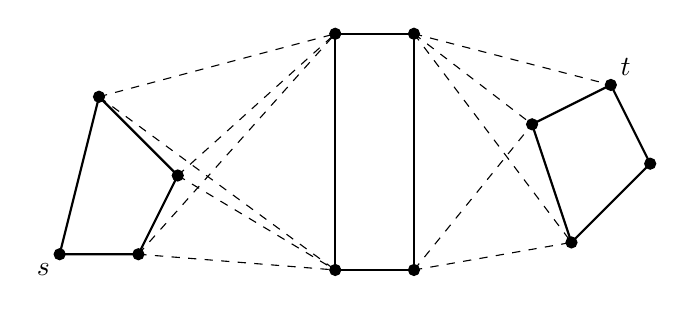
\begin{tikzpicture}
    % Variablen für das erste Polygon
    \coordinate (a0) at (0.5,0+0.2);
    \coordinate (a1) at (1,2+0.2);
    \coordinate (a2) at (2,1+0.2);
    \coordinate (a3) at (1.5,0+0.2);

    \filldraw (a0) circle (2pt);
    \filldraw (a1) circle (2pt);
    \filldraw (a2) circle (2pt);
    \filldraw (a3) circle (2pt);

    % Zeichne das erste Polygon
    \draw[thick] (a0) -- (a1) -- (a2) -- (a3) -- cycle;
    \node at (a0) [below left] {$s$};

    % Variablen für das Rechteck in der Mitte
    \coordinate (b0) at (4,0);
    \coordinate (b1) at (4,3);
    \coordinate (b2) at (5,3);
    \coordinate (b3) at (5,0);

    \filldraw (b0) circle (2pt);
    \filldraw (b1) circle (2pt);
    \filldraw (b2) circle (2pt);
    \filldraw (b3) circle (2pt);

    % Zeichne das Rechteck in der Mitte
    \draw[thick] (b0) -- (b1) -- (b2) -- (b3) -- cycle;


    % Variablen für das letzte Polygon
    \coordinate (c0) at (7,0+0.35);
    \coordinate (c1) at (8,1+0.35);
    \coordinate (c2) at (7.5,2+0.35);
    \coordinate (c3) at (6.5,1.5+0.35);

    \filldraw (c0) circle (2pt);
    \filldraw (c1) circle (2pt);
    \filldraw (c2) circle (2pt);
    \filldraw (c3) circle (2pt);

    % Zeichne das letzte Polygon
    \draw[thick] (c0) -- (c1) -- (c2) -- (c3) -- cycle;

    \node at (c2) [above right] {$t$};

    \draw[dashed] (a1) -- (b0);
    \draw[dashed] (a1) -- (b1);

    \draw[dashed] (a2) -- (b0);
    \draw[dashed] (a2) -- (b1);

    \draw[dashed] (a3) -- (b0);
    \draw[dashed] (a3) -- (b1);

    \draw[dashed] (b2) -- (c0);
    \draw[dashed] (b2) -- (c2);
    \draw[dashed] (b2) -- (c3);

    \draw[dashed] (b3) -- (c0);
    \draw[dashed] (b3) -- (c3);
  \end{tikzpicture}
  \caption{Beispiel Euclidean Shortest Path Problem}
  \label{fig:graphs:eulcidian_shotest_path_problem}
\end{figure}

\subsubsection{Eigenschaften}

Sichtbarkeitsgraphen sind im Allgemeinen \emph{nicht planar}.
Sie sind \emph{ungerichtet}, da die Sichtbarkeit zwischen zwei Punkten in beide Richtungen gilt.
Da die Gewichte der Kanten dem euklidischen Abstand zwischen den verbundenen Punkten entsprechen, bildet dieser eine untere Schranke des Abstandes für alle Knotenpaare, da ein kürzester Pfad durch das Umgehen von Hindernissen nur länger werden kann.

\subsubsection{Abgrenzung zu Straßengraphen}\label{graphs:strassengraphen}

Straßengraphen stellen eine spezielle Klasse von Graphen dar.
Eines ihrer auffälligsten Merkmale ist, dass sie nahezu planar sind, wobei Ausnahmen in Form von Brücken und Tunneln existieren.
Die Kantengewichte können etwa dem Luftlinienabstand oder der Reisezeit entsprechen, wobei sich letztere im Verlauf der Zeit ändert, etwa durch Stau oder Bauarbeiten.
Sie haben einen relativ geringen durchschnittlichen Knotengrad, denn Kreuzungen von mehr als zwei Straßen sind selten.

Sie besitzen eine hierarchische Struktur: Einfach gesagt, je schneller auf einer Straße gefahren werden darf, desto wichtiger ist diese für das Finden von kürzesten Pfaden.
Die Wichtigkeit der benutzten Straßen eines kürzesten Pfades steigt im Allgemeinen an, bis etwa eine Autobahn erreicht wird, und nimmt schließlich wieder ab, bis das Ziel erreicht wird.

Eine weitere Eigenschaft dieser hierarchischen Struktur ist, dass hinreichend lange Pfade durch ein vergleichsweise kleines Hitting-Set abgedeckt werden können, etwa durch alle Autobahnkreuze und Anschlussstellen.
Diese Beobachtung führt zur Definition der \emph{Highway Dimension}, einem Konzept, das von \cite{abraham2010highway} eingeführt wurde.

Aufgrund der unterschiedlichen Strukturen von Sichtbarkeitsgraphen und Straßengraphen können Algorithmen, die für Straßengraphen gute Laufzeiten aufweisen, zwar auf Sichtbarkeitsgraphen angewendet werden, allerdings ist ihre Rechenzeit häufig zu hoch, um eine effiziente Verarbeitung zu ermöglichen.

\subsubsection{Triangulierung}

Um die Distanzen zwischen Knotenpaaren in Sichtbarkeitsgraphen mit einer oberen Schranke abzuschätzen, kann eine \emph{Triangulierung} des Graphs durchgeführt werden, wie beispielsweise durch eine Delaunay-Triangulierung.
Dieser Ansatz kann jedoch lange, schmale Dreiecke erzeugen, die anschließend beseitigt werden können, um eine bessere obere Schranke zu erhalten.
Das Verfahren zur Erstellung der in dieser Arbeit verwendeten Triangulierung wird ausführlich von Funke et al. \cite{funkescalable} beschrieben.

Die Knoten eines triangulierten Graphen $G_g$ bilden hierbei eine Obermenge zur Menge der Knoten des dazugehörigen Sichtbarkeitsgraphen $G_v$.
Die Triangulation darf den kürzesten Pfad Abstand zweier Knoten $a, b$ nicht verkleinern, aber vergrößern.
\autoref{fig:thessaloniki_comparison} vergleicht einen Sichtbarkeitsgraphen und dessen Triangulierung anhand eines Ausschnitts.

\begin{figure}[h!]%
  \centering
  \subfloat[\centering{}aegaeis-graph]{{\includegraphics[width=.5\linewidth - 0.25cm]{img/thessaloniki-graph.png} }}%
  %\qquad
  \subfloat[\centering{}aegaeis-visibility]{{\includegraphics[width=.5\linewidth - 0.25cm]{img/thessaloniki-visibility.png} }}%
  \caption{Hafen von Thessaloniki}%
  \label{fig:thessaloniki_comparison}%
\end{figure}

\chapter{Contraction Hierarchies, Hierarchical Hub Labelings}\label{chapter:ch}

Mit dem Aufkommen von Online-Kartendiensten in den 2000er-Jahren stieg der Bedarf an effizienten Algorithmen zur Berechnung kürzester Pfade in großen Netzwerken stark an.
Klassische Algorithmen wie der Dijkstra-Algorithmus sind für sehr große Graphen, wie etwa Straßennetze von ganzen Kontinenten, aufgrund ihrer hohen Zeitkomplexität nicht praktikabel.
Um diesem Problem zu begegnen, führten Geisberger et al. \cite{geisberger2008contraction} die Methode der \emph{Contraction Hierarchies} ein.
Diese nutzt ein ähnliches Konzept wie die in \autoref{graphs:strassengraphen} vorgestellte Idee der Wichtigkeit von Kanten und ermöglicht auf Straßengraphen einen Speedup um mehrere Größenordnungen.

Aufbauend auf diesem Ansatz entwickelten Abraham et al. \cite{abraham2011hub} einen Algorithmus, welcher aus der von \emph{Contraction Hierarchies} erzeugten Datenstruktur ein \emph{Hub Labeling} erzeugt.
Hub-Labeling-Anfragen sind effektiv Look-Ups und können noch einmal um Größenordnungen schneller als Contraction-Hierarchies-Anfragen sein.

In diesem Kapitel werden die theoretischen Grundlagen dieser Methoden detailliert erläutert.
Zudem wird in \autoref{chapter:kontraktion}  die Anwendbarkeit dieser Techniken auf Sichtbarkeitsgraphen untersucht.

\section{Contraction Hierarchies}

Die grundlegende Idee von Contraction Hierarchies besteht darin, die Berechnung von kürzesten Wegen in großen Graphen, wie Straßennetzen, durch eine effiziente \emph{Vorverarbeitung} zu beschleunigen.

Während der Vorverarbeitung werden die Knoten des Graphen in einer bestimmten Reihenfolge \emph{kontrahiert}, was bedeutet, dass sie entfernt werden.
Beim Entfernen eines Knotens werden \emph{Abkürzungen} zwischen seinen Nachbarn hinzugefügt, um sicherzustellen, dass die Abstände im übrigen Graphen erhalten bleiben.
Diese Abkürzungen ersetzen längere Pfade, die über den entfernten Knoten geführt hätten.

Durch die Kontraktion entsteht eine Hierarchie der Knoten, wobei \emph{weniger wichtige Knoten} zuerst kontrahiert werden.
Bei der eigentlichen Anfrage wird ein modifizierter bidirektionaler Dijkstra-Algorithmus verwendet, der die Hierarchie ausnutzt.
Die Suche beschränkt sich auf Kanten, die \emph{aufwärts} in der Hierarchie führen, was die Anzahl der während der Suche gesehenen Knoten stark reduzieren \emph{kann}.

\subsection{Knoten-Kontraktion}

Der Begriff Contraction Hierarchies leitet sich vom Konzept der Knoten-Kontraktion ab.

\begin{definition}[Knoten-Kontraktion]
  Sei $G = (V, E)$ ein Graph. Sei $v \in V$ der zu kontrahierende Knoten. Die Kontraktion von $v$ erfolgt in zwei Schritten:

  \begin{enumerate}
    \item\label{ch:contraction:when_shortcut}
    Für jeden Vorgänger $u \in V$ und jeden Nachfolger $w \in V$ von $v$ wird, wenn $(u, v, w)$ der einzige kürzeste $u$-$w$-Pfad ist, eine Abkürzung $(u, w, {spd}_G((u, w)))$ zu $E$ hinzugefügt.

    \item
          Alle Kanten von und zu $v$ werden entfernt.
  \end{enumerate}
\end{definition}

Nach der Kontraktion $v$ ist somit isoliert.
Um die Abkürzungen zu erzeugen, kann von jedem Vorgänger eine modifizierte Dijkstra-Suche zu allen Nachfolgern ausgeführt werden, bei der die $(v, w)$ Kanten nicht begangen wird.
Ist die Länge der potenziellen Abkürzung kürzer als die des in der modifizierten Dijkstra-Suche gefundenen Pfades, so ist $(u, v, w)$ der einzige kürzeste $u$-$w$-Pfad.
Die Knoten-Kontraktion bewahrt daher Abstände zwischen den verbleibenden Knoten.

Dies lässt sich am ungerichteten Beispielgraphen veranschaulichen.
Sei $i$ der zu kontrahierende Knoten, dessen Nachbarn $a$, $b$, $j$ und $h$ sind.
Die kürzesten $a$-$b$-, $b$-$j$-, $h$-$j$- und $a$-$h$-Pfade führen nicht durch $i$.
Der kürzeste $a$-$j$-Pfad ist $(a, i, j)$,daher wird eine Kante zwischen $a$ und $j$ eingefügt.
\autoref{graphs:fig:example_contraction} zeigt den Graphen vor und nach der Kontraktion.

\begin{figure}[h!]
  \centering
  \begin{subfigure}[b]{0.49\textwidth}
    \centering
    \resizebox{\textwidth}{!}{% <------ Don't forget this %
      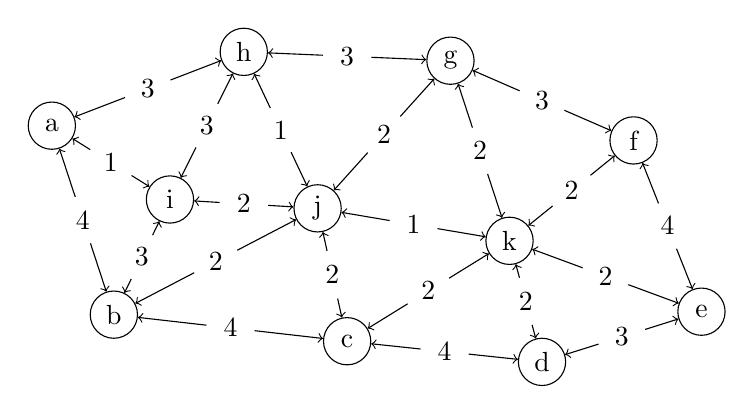
\begin{tikzpicture}[scale=0.750]
        \node[circle, draw, minimum size=0.6cm, inner sep=0pt] at (0.5* 0.0, 0.5* 8.5)  (a)    {a};
        \node[circle, draw, minimum size=0.6cm, inner sep=0pt] at (0.5* 2.1, 0.5* 2.1)  (b)    {b};
        \node[circle, draw, minimum size=0.6cm, inner sep=0pt] at (0.5* 10.0, 0.5* 1.2)  (c)    {c};
        \node[circle, draw, minimum size=0.6cm, inner sep=0pt] at (0.5* 16.6, 0.5* 0.5)  (d)    {d};
        \node[circle, draw, minimum size=0.6cm, inner sep=0pt] at (0.5* 22.0, 0.5* 2.2)  (e)    {e};
        \node[circle, draw, minimum size=0.6cm, inner sep=0pt] at (0.5* 19.7, 0.5* 8.0)  (f)    {f};
        \node[circle, draw, minimum size=0.6cm, inner sep=0pt] at (0.5* 13.5, 0.5* 10.7)  (g)    {g};
        \node[circle, draw, minimum size=0.6cm, inner sep=0pt] at (0.5* 6.5, 0.5* 11.0)  (h)    {h};
        \node[circle, draw, minimum size=0.6cm, inner sep=0pt] at (0.5* 4.0, 0.5* 6.0)  (i)    {i};
        \node[circle, draw, minimum size=0.6cm, inner sep=0pt] at (0.5* 9.0, 0.5* 5.7)  (j)    {j};
        \node[circle, draw, minimum size=0.6cm, inner sep=0pt] at (0.5* 15.5, 0.5* 4.6)  (k)    {k};

        \draw[<->]  (a) edge node[circle, fill=white] {4} (b);
        \draw[<->]  (a) edge node[circle, fill=white] {3} (h);
        \draw[<->]  (a) edge node[circle, fill=white] {1} (i);

        \draw[<->]  (b) edge node[circle, fill=white] {4} (c);
        \draw[<->]  (b) edge node[circle, fill=white] {3} (i);
        \draw[<->]  (b) edge node[circle, fill=white] {2} (j);

        \draw[<->]  (c) edge node[circle, fill=white] {4} (d);
        \draw[<->]  (c) edge node[circle, fill=white] {2} (j);
        \draw[<->]  (c) edge node[circle, fill=white] {2} (k);

        \draw[<->]  (d) edge node[circle, fill=white] {3} (e);
        \draw[<->]  (d) edge node[circle, fill=white] {2} (k);

        \draw[<->]  (e) edge node[circle, fill=white] {4} (f);
        \draw[<->]  (e) edge node[circle, fill=white] {2} (k);

        \draw[<->]  (f) edge node[circle, fill=white] {3} (g);
        \draw[<->]  (f) edge node[circle, fill=white] {2} (k);

        \draw[<->]  (g) edge node[circle, fill=white] {3} (h);
        \draw[<->]  (g) edge node[circle, fill=white] {2} (j);
        \draw[<->]  (g) edge node[circle, fill=white] {2} (k);

        \draw[<->]  (h) edge node[circle, fill=white] {3} (i);
        \draw[<->]  (h) edge node[circle, fill=white] {1} (j);

        \draw[<->]  (i) edge node[circle, fill=white] {2} (j);

        \draw[<->]  (j) edge node[circle, fill=white] {1} (k);
      \end{tikzpicture}
    }
    \caption{Vor der Kontraktion}
  \end{subfigure}
  \hfill
  \begin{subfigure}[b]{0.49\textwidth}
    \centering
    \resizebox{\textwidth}{!}{% <------ Don't forget this %
      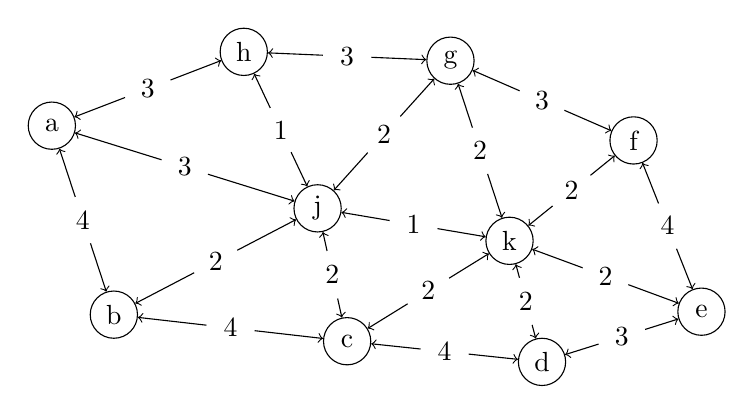
\begin{tikzpicture}[scale=0.750]
        % Nodes
        \node[circle, draw, minimum size=0.6cm, inner sep=0pt] at (0.5* 0.0, 0.5* 8.5)  (a)    {a};
        \node[circle, draw, minimum size=0.6cm, inner sep=0pt] at (0.5* 2.1, 0.5* 2.1)  (b)    {b};
        \node[circle, draw, minimum size=0.6cm, inner sep=0pt] at (0.5* 10.0, 0.5* 1.2)  (c)    {c};
        \node[circle, draw, minimum size=0.6cm, inner sep=0pt] at (0.5* 16.6, 0.5* 0.5)  (d)    {d};
        \node[circle, draw, minimum size=0.6cm, inner sep=0pt] at (0.5* 22.0, 0.5* 2.2)  (e)    {e};
        \node[circle, draw, minimum size=0.6cm, inner sep=0pt] at (0.5* 19.7, 0.5* 8.0)  (f)    {f};
        \node[circle, draw, minimum size=0.6cm, inner sep=0pt] at (0.5* 13.5, 0.5* 10.7)  (g)    {g};
        \node[circle, draw, minimum size=0.6cm, inner sep=0pt] at (0.5* 6.5, 0.5* 11.0)  (h)    {h};
        % \node[circle, draw, minimum size=0.6cm, inner sep=0pt] at (0.5* 4.0, 0.5* 6.0)  (i)    {i};
        \node[circle, draw, minimum size=0.6cm, inner sep=0pt] at (0.5* 9.0, 0.5* 5.7)  (j)    {j};
        \node[circle, draw, minimum size=0.6cm, inner sep=0pt] at (0.5* 15.5, 0.5* 4.6)  (k)    {k};

        \draw[<->]  (a) edge node[circle, fill=white] {4} (b);
        \draw[<->]  (a) edge node[circle, fill=white] {3} (h);
        \draw[<->]  (a) edge node[circle, fill=white] {3} (j);

        \draw[<->]  (b) edge node[circle, fill=white] {4} (c);
        \draw[<->]  (b) edge node[circle, fill=white] {2} (j);

        \draw[<->]  (c) edge node[circle, fill=white] {4} (d);
        \draw[<->]  (c) edge node[circle, fill=white] {2} (j);
        \draw[<->]  (c) edge node[circle, fill=white] {2} (k);

        \draw[<->]  (d) edge node[circle, fill=white] {3} (e);
        \draw[<->]  (d) edge node[circle, fill=white] {2} (k);

        \draw[<->]  (e) edge node[circle, fill=white] {4} (f);
        \draw[<->]  (e) edge node[circle, fill=white] {2} (k);

        \draw[<->]  (f) edge node[circle, fill=white] {3} (g);
        \draw[<->]  (f) edge node[circle, fill=white] {2} (k);

        \draw[<->]  (g) edge node[circle, fill=white] {3} (h);
        \draw[<->]  (g) edge node[circle, fill=white] {2} (j);
        \draw[<->]  (g) edge node[circle, fill=white] {2} (k);

        \draw[<->]  (h) edge node[circle, fill=white] {1} (j);

        \draw[<->]  (j) edge node[circle, fill=white] {1} (k);
      \end{tikzpicture}
    }
    \caption{Nach der Kontraktion}
  \end{subfigure}
  \caption{Kontraktion von $i$}
  \label{graphs:fig:example_contraction}
\end{figure}

Häufig wird die Kontraktionsbedingung abgeschwächt, indem dann eine Kante eingefügt wird, wenn der zu kontrahierende Knoten auf \emph{einem} kürzesten Pfad liegt.
Dazu kann eine normale Dijkstra-Suche verwendet werden: Ist die Länge einer potenziellen Abkürzung optimal, dann wird sie eingefügt.
Da die Suche, die $(v, w)$ nicht durchläuft, den gesamten Graphen absucht wenn $(u, v, w)$ der einzige $u$-$w$-Pfad ist, kann dies sehr effektiv sein.
Weiter kann die Anzahl der Hops der Suche begrenzt werden.
Dadurch können jedoch auch Kanten eingefügt werden, die nicht unbedingt für die Erhaltung der Abstände erforderlich sind.

\subsection{Graphen-Kontraktion}

Um die Datenstruktur für die Beantwortung von Anfragen, den \emph{Contracted-Graph}, zu erstellen, müssen alle Knoten eines Graphen kontrahiert werden. Die Kanten, die in jedem Schritt entfernt werden, werden dabei gesammelt.
Hierbei hat die Reihenfolge, in der das geschieht, einen großen Einfluss auf Performance der nachfolgenden Kontraktionen und den mit der Methode erzielte Speedup.
Die Reihenfolge der Kontraktion wird durch eine \emph{vertex-to-level}-Funktion angegeben.
Sie ist bijektiv und definiert als ${vtl} \colon V \to L$ mit $L \subset \mathbb{N}$, $\abs{L} = \abs{V}$ und $\max(L) = \abs{V}$.
Der Knoten mit dem niedrigsten \emph{Level} wird dabei zuerst kontrahiert.
Ihre Umkehrfunktion wird \emph{level-to-vertex}-Funktion genannt.

\begin{definition}[Contracted-Graph]
  Sei $G = (V, E)$ und $E'$ die durch die vollständige Kontraktion von $G$ erhaltenen Kanten mit der dazugehörigen vertex-to-level-Funktion ${vtl}$.

  Ein Contracted-Graph ist dann ein Tupel $C = (G_u, G_d)$. Der \emph{Upward-Graph} ist dabei $G_u = (V, E_u)$ mit $E_u = \{ (t, h) \mid (t, h) \in E' \colon {vtl}(h) > {vtl}(t) \}$, der \emph{Downward-Graph} ist $G_d = (V, E_d)$ mit $E_d = \{ (h, t) \mid (t, h) \in E' \colon {vtl}(h) < {vtl}(t) \}$.
\end{definition}

Der Name Upward-Graph leitet sich daraus ab, dass die Suche innerhalb dieses Graphen bezogen auf die Level ausschließlich \emph{aufwärts} erfolgt.
In \cite{geisberger2008contraction} transponieren die Autoren die Kanten des Downward-Graph nicht, daher geht ihre Suche \emph{abwärts}.
Die Transposition der Kanten ist hierbei nur eine Methode, damit auf dem Downward-Graphen wie auf dem Upward-Graphen \emph{vorwärts} gesucht wird.

Der entstandene Graph ist azyklisch, da er nur Kanten enthält, deren Kopf ein größeres Level als der dazugehörige Fuß hat.
Die Anzahl der in einer Breitensuche gefundenen Knoten ist geringer als im Ursprungsgraph.
Diese Eigenschaften sorgen dafür, dass eine Suche in einem Upward-Graph kostengünstiger sein kann.
Die kürzesten Pfade, die im Upward-Graph gefunden worden, bilden eine obere Schranke für die tatsächlich kürzesten Pfade in $G$, in einigen Fällen können sie jedoch länger sein.
\autoref{graphs:fig:counterexample_optimal_Upward} zeigt ein Beispiel hierzu.
Die Knoten sind in der Reihenfolge $c$, $d$, $a$, $b$ kontrahiert worden, wodurch der dazugehörige Upward-Graph entsteht.
Der optimale $c$-$a$-Pfad in $G$ hat die Distanz zwei, in $G_u$ hat er jedoch die Distanz drei.

\begin{figure}[ht]
  \centering
  \begin{subfigure}[b]{0.49\textwidth}
    \centering
    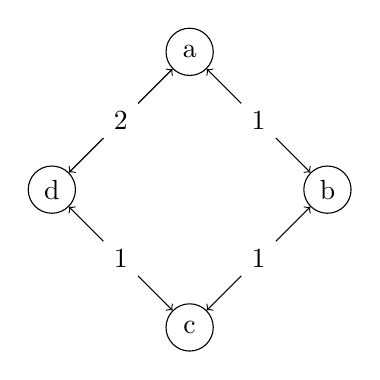
\begin{tikzpicture}
      \node[circle, draw, minimum size=0.6cm, inner sep=0pt] at (1.75*1.0, 1.75*2.0)  (a)    {a};
      \node[circle, draw, minimum size=0.6cm, inner sep=0pt] at (1.75*2.0, 1.75*1.0)  (b)    {b};
      \node[circle, draw, minimum size=0.6cm, inner sep=0pt] at (1.75*1.0, 1.75*0.0)  (c)    {c};
      \node[circle, draw, minimum size=0.6cm, inner sep=0pt] at (1.75*0.0, 1.75*1.0)  (d)    {d};

      \draw[<->]  (a) edge node[circle, fill=white] {1} (b);
      \draw[<->]  (b) edge node[circle, fill=white] {1} (c);
      \draw[<->]  (c) edge node[circle, fill=white] {1} (d);
      \draw[<->]  (d) edge node[circle, fill=white] {2} (a);
    \end{tikzpicture}
    \caption{Graph $G$}
  \end{subfigure}
  \hfill
  \begin{subfigure}[b]{0.49\textwidth}
    \centering
    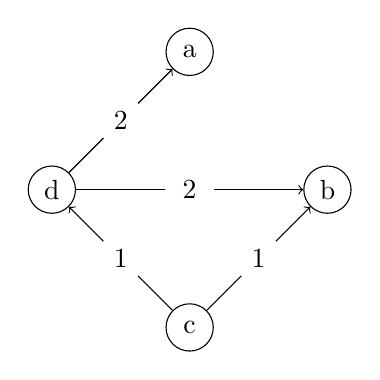
\begin{tikzpicture}
      \node[circle, draw, minimum size=0.6cm, inner sep=0pt] at (1.75*1.0, 1.75*2.0)  (a)    {a};
      \node[circle, draw, minimum size=0.6cm, inner sep=0pt] at (1.75*2.0, 1.75*1.0)  (b)    {b};
      \node[circle, draw, minimum size=0.6cm, inner sep=0pt] at (1.75*1.0, 1.75*0.0)  (c)    {c};
      \node[circle, draw, minimum size=0.6cm, inner sep=0pt] at (1.75*0.0, 1.75*1.0)  (d)    {d};

      \draw[->]  (c) edge node[circle, fill=white] {1} (b);
      \draw[->]  (c) edge node[circle, fill=white] {1} (d);
      \draw[->]  (d) edge node[circle, fill=white] {2} (b);
      \draw[->]  (d) edge node[circle, fill=white] {2} (a);
    \end{tikzpicture}
    \caption{Upward-Graph $G_u$ zu $G$}
  \end{subfigure}
  \caption{Gegenbeispiel optimale Kosten im $G_u$}
  \label{graphs:fig:counterexample_optimal_Upward}
\end{figure}

\subsection{Anfragen}

Die Suche eines kürzesten Pfades von $a$ nach $e$ auf dem Beispielgraphen gestaltet sich nun wie folgt:
Auf $G_u$ wird eine Dijkstra-Suche von $a$ und auf $G_d$ eine Dijkstra-Suche von $e$ durchgeführt.
Aus den von beiden Dijkstra-Suchen besuchten Knoten wird nun derjenige ausgewählt, der die niedrigste Summe beider Distanzen aufweist.
\autoref{fig:ch:beispiel_suche} zeigt den auf diese Weise gefundenen Pfad im Beispielgraphen von $a$ nach $e$.
Die Level der Knoten auf dem Pfad steigen von beiden Seiten an, bis sie den Treffpunktknoten $j$ erreichen.
Hierbei ist die Kante $(a, j)$ eine Abkürzung, sie kürzt $i$ ab, was durch die gestrichelten Pfeile angedeutet wird.

\begin{figure}[ht]
  \centering
  \begin{tikzpicture}
    \node[circle, draw] at (0 * 1.5, -2 * 0.75)  (a)    {a};
    \node[circle, draw] at (1 * 1.5, -4 * 0.75)  (i)    {i};
    \node[circle, draw] at (2 * 1.5, -0 * 0.75)  (j)    {j};
    \node[circle, draw] at (3 * 1.5, -1 * 0.75)  (k)    {k};
    \node[circle, draw] at (4 * 1.5, -3 * 0.75)  (e)    {e};

    % draw axis
    \draw[->] (-1, -4 * 0.75) -- (-1, 0) node[above] {Level};

    \draw[->]  (a) -- (j);
    \draw[->]  (e) -- (k);
    \draw[->]  (k) -- (j);

    \draw[->, dotted]  (a) -- (i);
    \draw[->, dotted]  (i) -- (j);

  \end{tikzpicture}
  \caption{Beispiel einer Suche im Contrated Graph}
  \label{fig:ch:beispiel_suche}
\end{figure}

Algorithmus \ref{ch:query_simple} definiert dies formal.
Wie bei einer bidirektionalen Dijkstra-Suche wird der Pfad, sofern existent, aus den Teilpfaden beider Suchen erstellt.
Diese haben die Form $(u, \dotsc, t)$ beziehungsweise $(v, \dotsc, t)$.
Um einen gültigen Pfad zu erstellen, muss $t$ aus einem dieser Teilpfade entfernt und der Pfad des Downward-Graphen umgekehrt werden.
Anschließend können beide Pfade konkateniert werden, somit entsteht ein Pfad auf $C$ der Form $(u, \dotsc, t, \dotsc, v)$.
Dieser muss jedoch nicht unbedingt ein gültiger Pfad auf $G$ sein, da er noch Abkürzungen enthalten kann.
In \autoref{ch:subsection:pfad_gewinnung} wird darauf eingegangen, wie diese entfernt werden können.

\begin{algorithm}[ht]
  \caption{Construction Hierarchies Query}
  \begin{algorithmic}[1]
    \Require Upward-Graph $G_u = (V, E_u)$, Downward-Graph $G_d = (V, E_d)$, Startknoten $s \in V$, Zielknoten $t \in V$
    \Ensure Treffknoten $m \in V \cup \{ {none} \}$, ${dist}_u$, ${pre}_u$, ${dist}_d$, ${pre}_d$
    \State ${dist}_u$, ${pre}_u$ $\leftarrow$ Dijkstra$(G_u, s)$
    \State ${dist}_d$, ${pre}_d$ $\leftarrow$ Dijkstra$(G_d, t)$

    \State
    \State $m \leftarrow {none}$
    \State $d \leftarrow \infty$
    \State
    \ForAll {$v \in V$}
    \If {${dist}_u(v) + {dist}_d(v) < d$}
    \State $m \leftarrow v$
    \State $d \leftarrow {dist}_u(v) + {dist}_d(v)$
    \EndIf
    \EndFor

    \State
    \State \Return $m$, ${dist}_u$, ${pre}_u$, ${dist}_d$, ${pre}_d$
  \end{algorithmic}
  \label{ch:query_simple}
\end{algorithm}

Die Korrektheit des Algorithmus ist nicht sofort ersichtlich, da nicht alle besuchten Knoten eine optimal Distanz haben und nur ein Teil aller Knoten besucht wird.
Der Beweis hierfür betrachtet einen kürzesten Pfad auf $G$ und argumentiert, warum dieser gefunden wird:


\begin{beweis}[Korrektheit der Contracted-Graph-Anfrage]\label{ch:proof:correct}
  Der Upward-Graph $G_u$ und der Downward-Graph $G_d$ enthalten nur Kanten, die mindestens so lang sind wie der Abstand in $G$.
  Daher kann ein $s$-$t$-Pfad in $C$ nur dann gefunden werden, wenn auch in $G$ ein solcher Pfad existiert.

  Es ist zu zeigen, dass eine Suche auf $C$ den Abstand in $G$ liefert.
  Sei $\text{sp}_G(s, t)$ ein kürzester Pfad auf $G$, der unter allen kürzesten Pfaden den Knoten $m$ mit dem höchsten Level enthält.
  Aus diesem Pfad $(s, \dotsc, t)$ werden zwei Teilpfade konstruiert: $(s, \dotsc, m)$ und $(t, \dotsc, m)$.

  Betrachte den Teilpfad $(s, \dotsc, m)$ mit der Hop-Länge $n_u$.
  Entferne aus diesem Pfad alle Knoten zwischen $s$ und $m$, die ein kleineres Level als ihre Vorgänger haben.
  Dieser Vorgang wird so oft wiederholt, bis keine weiteren Knoten mehr entfernt werden können.

  Der resultierende Pfad besteht aus überlappenden Tupeln der Form $(v_{i}, v_{i + 1})$.
  Für diese gilt $\text{vtl}(v_i) < \text{vtl}(v_{i + 1})$, da sich der Pfad im Upward-Graph befindet.
  Die Knoten-Kontraktion erhält die Abstände der verbleibenden Knoten.
  Zum Zeitpunkt der Kontraktion von $v_i$ existierte also ein optimaler Pfad von $v_i$ zu $v_{i + 1}$.
  Alle Knoten, die ursprünglich zwischen ihnen lagen und entfernt wurden, haben ein kleineres Level als $v_i$ und waren zum Zeitpunkt der Kontraktion von $v_i$ bereits kontrahiert.
  Daher existierte vor der Kontraktion von $v_i$ eine direkte Kante zu $v_{i + 1}$, die gesammelt und zum Aufbau des Upward-Graphen verwendet wurde.
  Somit wird $v_{i + 1}$ von $v_i$ aus erreicht.
  Da dies für alle überlappenden Tupel gilt, wird $m$ von $s$ aus mit optimalem Abstand erreicht.

  Analog wird für den Teilpfad $(t, \dotsc, m)$ im Downward-Graph argumentiert.
  \qed
\end{beweis}

\subsection{Erstellung des Pfades}\label{ch:subsection:pfad_gewinnung}

Der in $C$ gefundene Pfad kann noch Abkürzungen enthalten.
Damit der Pfad auch auf $G$ gültig ist, müssen diese ersetzt werden.
Hierfür ist eine Funktion notwendig, welche diese ersetzt.

Eine solche Abkürzungsfunktion kann etwa durch eine HashMap implementiert werden.
Da die ${vtl}$-Funktion bijektiv ist, gilt für alle Knoten $u, v \in V$, $u \neq v$ immer entweder ${vtl}(u) < {vtl}(v)$ oder ${vtl}(u) > {vtl}(v)$.
Daher reicht es für die Ersetzung der Abkürzungen in Pfaden in $C$ \emph{eine} HashMap zu benutzen, da keine Kollisionen zwischen Abkürzungen des Upward- und des Downward-Graphen entstehen können.

\begin{figure}[ht]
  \centering
  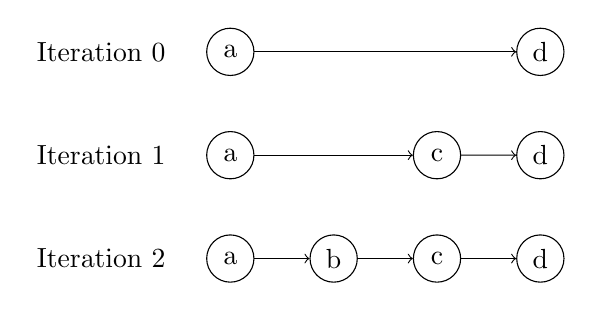
\begin{tikzpicture}[scale=0.75]
    \node[align=left] at (1.75*-1.25,1.75*2) {Iteration 0};
    \node[circle, draw, minimum size=0.6cm, inner sep=0pt] at (1.75*0.0, 1.75*2.0)  (a_0)    {a};
    \node[circle, draw, minimum size=0.6cm, inner sep=0pt] at (1.75*3.0, 1.75*2.0)  (d_0)    {d};
    \draw[->]  (a_0) edge node {} (d_0);

    \node[align=left] at (1.75*-1.25,1.75*1) {Iteration 1};
    \node[circle, draw, minimum size=0.6cm, inner sep=0pt] at (1.75*0.0, 1.75*1.0)  (a_1)    {a};
    \node[circle, draw, minimum size=0.6cm, inner sep=0pt] at (1.75*2.0, 1.75*1.0)  (c_1)    {c};
    \node[circle, draw, minimum size=0.6cm, inner sep=0pt] at (1.75*3.0, 1.75*1.0)  (d_1)    {d};
    \draw[->]  (a_1) edge node {} (c_1);
    \draw[->]  (c_1) edge node {} (d_1);

    \node[align=left] at (1.75*-1.25,1.75*0) {Iteration 2};
    \node[circle, draw, minimum size=0.6cm, inner sep=0pt] at (1.75*0.0, 1.75*0.0)  (a_2)    {a};
    \node[circle, draw, minimum size=0.6cm, inner sep=0pt] at (1.75*1.0, 1.75*0.0)  (b_2)    {b};
    \node[circle, draw, minimum size=0.6cm, inner sep=0pt] at (1.75*2.0, 1.75*0.0)  (c_2)    {c};
    \node[circle, draw, minimum size=0.6cm, inner sep=0pt] at (1.75*3.0, 1.75*0.0)  (d_2)    {d};
    \draw[->]  (a_2) edge node {} (b_2);
    \draw[->]  (b_2) edge node {} (c_2);
    \draw[->]  (c_2) edge node {} (d_2);
  \end{tikzpicture}
  \caption{Beispiel des iterativen Ersetzen von Abkürzungen}
\end{figure}

Um diese Funktion zu erhalten, müssen die Abkürzungen, welche beim Kontrahieren des Graphen eingefügt werden, und die dabei übersprungenen Knoten gesammelt werden.
Einen möglichen Algorithmus, der Abkürzungen in einem Pfad ersetzt, ist in Algorithmus \ref{ch:alg:shortcut_replacement} zu sehen.
Dieser betrachtet den Pfad mit Abkürzungen als Stapel und bearbeitet jeweils nur die beiden obersten Knoten, weil das Einfügen an einer bestimmten Stelle in ein Array rechenintensiv ist.

\begin{algorithm}[ht]
  \caption{Shortcut replacement}
  \begin{algorithmic}[1]
    \Require Pfad $p$ mit Abkürzungen, Abkürzungungsfunktion $S \colon V \times V \to V \cup \{ {none} \}$
    \Ensure Pfad $p'$ ohne Shortcuts

    \If {$\text{len}(p) == 1$}
    \State \Return $p$
    \EndIf
    \State

    \State $p' \leftarrow ()$
    \State

    \While {$\text{len}(p) >= 2$}
    \State $w \leftarrow \text{pop}(p)$
    \State $u \leftarrow \text{pop}(p)$
    \State $v \leftarrow S((u, w))$
    \State

    \If {$v \neq none$}
    \State $\text{push}(p, u)$
    \State $\text{push}(p, v)$
    \State $\text{push}(p, w)$
    \Else
    \State $\text{push}(p, u)$
    \State $\text{push}(p', w)$
    \EndIf
    \EndWhile

    \State
    \State $p' \leftarrow \text{reversed}(p')$

    \State
    \State \Return $p'$
  \end{algorithmic}
  \label{ch:alg:shortcut_replacement}
\end{algorithm}

\subsection{Early stop}

Algorithmus \ref{ch:query_simple} hat primär theoretische Bedeutung.
Implementierungen ähneln der bidirektionalen Dijkstra-Suche, dabei werden abwechselnd Knoten der Upward-Suche und der Downward-Suche expandiert
Die Expansion einer Suchrichtung wird gestoppt, wenn die kleinste Distanz der Vorwärtswarteschlange größer als die bisherige kleinste Treffpunkt-Distanz ist.
Sobald beide Suchen gestoppt wurden, ist der kürzeste Pfad, falls vorhanden, gefunden.

\subsection{stall-on-demand}

Wie \autoref{graphs:fig:counterexample_optimal_Upward} zeigt, sind manche der im Upward- und Downward-Graphen gefundenen Distanzen nicht optimal.
Für das Finden eines kürzesten Pfades sind jedoch nur die Knoten interessant, deren Distanz optimal ist.
Mit der von \cite{schultes2007dynamic} vorgestellten Methode \emph{stall-on-demand} ist es möglich, den Suchraum der beiden Teilsuchen einzuschränken.
Hierfür wird die Expansion eines Knotens abgebrochen, wenn er über eine Kante des jeweils anderen Graphen günstiger erreicht werden kann.

\begin{definition}[stall-on-demand]
  Sei $C = (G_u, G_d)$ ein Contracted-Graph mit $G_u = (V, E_u)$ und $G_d = (V, E_d)$.
  Der Knoten $u \in V$ hat keine optimale Distanz in der Dijkstra-Suche von $s$ in $G_u$, wenn es zum Zeitpunkt seiner Expansion eine Kante $(u, v, d) \in E_d$, $v \in V$, $d \in \mathbb{R}$ gibt mit ${dist}(v) + d < {dist}(u)$.
  Die Expansion von $u$ kann dann abgebrochen werden, die aus $u$ ausgehenden Kanten müssen nicht betrachtet werden.
  Gleiches gilt analog für $G_d$.
\end{definition}

Veranschaulicht wird dies an dem Beispiel in \autoref{fig:ch:stall_example}.
Wir befinden uns in der Suche des Upward-Graphen.
Die blauen Kanten repräsentieren Kanten der Upward-Suche, während die rote Kante eine von $u$ ausgehende Downward-Kante darstellt.
Bisher wurde $v$ in der Upward-Suche mit einer Distanz von eins expandiert, im nächsten Schritt soll $u$ expandiert werden.
Der Knoten $u$ hat die Distanz drei in der Upward-Suche, kann jedoch über die Upward-Kante mit einer Distanz von zwei erreicht werden.
Also ist die Distanz drei nicht optimal, und von $u$ ausgehenden Kanten müssen nicht betrachtet werden.

\begin{figure}
  \centering
  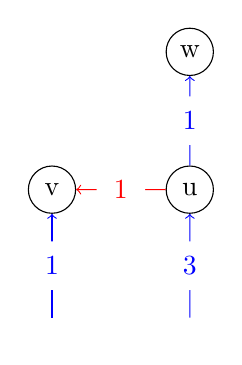
\begin{tikzpicture}[scale=1.75]
    \node[circle, draw, minimum size=0.6cm, inner sep=0pt] at (0, 2)  (v)    {v};
    \node[circle, draw, minimum size=0.6cm, inner sep=0pt] at (1, 2)  (u)    {u};
    \node[circle, draw, minimum size=0.6cm, inner sep=0pt] at (1, 3)  (w)    {w};

    \node[] at (0, 1)  (uv)    {};
    \node[] at (1, 1)  (uu)    {};

    \draw[->,blue]  (u) edge node[circle, fill=white] {1} (w);

    \draw[->,red]  (u) edge node[circle, fill=white] {1} (v);

    \draw[->,blue]  (uv) edge node[circle, fill=white] {1} (v);
    \draw[->,blue]  (uu) edge node[circle, fill=white] {3} (u);
  \end{tikzpicture}
  \caption{Beispiel stall-on-demand}
  \label{fig:ch:stall_example}
\end{figure}

\subsection{Erstellung}

Ein Contracted-Graph entsteht durch die vollständige Kontraktion eines Graphen.
Die Reihenfolge, in der die Knoten kontrahiert werden, kann im Voraus festgelegt werden, oder der jeweils \emph{unwichtigste} Knoten wird kontrahiert.
Der Prozess der Erstellung kann nach mehreren Kriterien bewertet werden, so kann die Geschwindigkeit der Erstellung, die Geschwindigkeit der Anfragen oder die Anzahl der bei der Kontraktion hinzugefügten Abkürzungen minimiert werden.

\subsubsection{Top-Down}
Bei der Top-Down-Kontraktion ist die level-to-vertex-Funktion ${ltv}$ vorgegeben.
Die Knoten werden in der Reihenfolge ihres Levels kontrahiert, wobei mit dem niedrigsten Level begonnen wird.
Diese Herangehensweise bietet die Möglichkeit dafür eine optimale Reihenfolge anzuwenden, wobei sie für hinreichend große Graphen nur schwer bestimmbar ist.

Bei der \emph{Sortierung nach Grad} werden die Knoten nach ihrem Grad sortiert, wobei die Knoten mit den kleinsten Graden zuerst kontrahiert werden.
Die Überlegung dahinter ist, dass Knoten mit vielen Nachbarn auch viele neue Kanten einfügen können, was vermieden werden soll.

Die Knoten können auch über ein Hitting-Set sortiert werden:
Hierbei wird auf Grundlage einer möglichst großen Anzahl von Pfaden ein Hitting-Set gebildet.
Die Knoten des Hitting-Sets werden dann nach der Anzahl ihrer Hits sortiert.
Den Knoten, die nicht Teil des Hitting-Sets sind, werden anschließend die unteren Level zugewiesen, wobei diese wiederum nach einer Metrik wie etwa dem Grad sortiert werden können.

\subsubsection{Bottom-Up}

Bei der Bottom-Up-Kontraktion wird die vertex-to-level-Funktion ${vtl}$ während der Kontraktion erstellt.
Dabei wird mithilfe einer Heuristik der jeweils \emph{unwichtigste} Knoten aus einer Prioritätswarteschlange ausgewählt und kontrahiert.
Ein unwichtiger Knoten hat einen niedrigen Heuristikwert.
Die in der Praxis am häufigsten verwendeten Heuristiken beinhalten die \emph{Kanten-Differenz}, berücksichtigen jedoch häufig auch weitere Informationen.

Die Kanten-Differenz gibt an, wie sich die Anzahl der Kanten im gesamten Graphen durch die Kontraktion eines Knotens verändert.
Sie wird berechnet, indem die Anzahl der neu hinzugefügten Kanten von der Anzahl der entfernten Kanten subtrahiert wird, wobei die Kontraktion des Knotens \emph{simuliert} wird.
Die Kontraktion eines Knotens kann die Heuristikwerte anderer Knoten beeinflussen.
Um sicherzustellen, dass stets der Knoten mit dem niedrigsten Heuristikwert ausgewählt wird, müssten nach jeder Kontraktion alle Heuristikwerte neu berechnet werden.
Da dies jedoch in der Praxis zu teuer ist, haben sich zwei Methoden als effektiv erwiesen:

Beim \emph{Lazy-Popping} wird angenommen, dass ein Knoten nur an Wichtigkeit gewinnen kann.
Aus der Warteschlange wird ein Knoten entnommen und geprüft, ob sein Heuristikwert gestiegen ist.
Falls er gestiegen ist, wird er zurück in die Warteschlange geschoben, andernfalls wird er kontrahiert.
Dies wird wiederholt, bis ein Knoten gefunden wird, dessen Heuristikwert unverändert geblieben ist.
Beim \emph{Neighbor-Update} werden nach der Kontraktion eines Knotens die Heuristikwerte der benachbarten Knoten aktualisiert.

Um die zu einem Contracted-Graph gehörende Abkürzungsfunktion zu erhalten, muss während der Kontraktion des Graphen eine Liste der Abkürzungen erstellt werden.
Wenn die im vorherigen Abschnitt erwähnte abgeschwächte Bedingung verwendet wird, muss sichergestellt werden, dass sich die Abkürzungen zweier Knoten während der Kontraktion mehrmals ändern können.
Dabei darf nur die letzte und beste Abkürzung gespeichert werden.

\section{Hierarchical Hub Labeling}\label{chapter:hl}

Die Contracted-Graph-Anfrage ohne Stopbedingung baut jeweils den vollständigen Suchbaum für den Start- und Zielknoten auf und sucht aus den expandierten Knoten beider Suchen den Knoten mit der geringsten Summe der Distanzen in beiden Suchen.
Die Idee hinter dem Labeling besteht darin, den Suchbaum des Upward- bzw. Downward-Graphen zu speichern, sodass eine $s$-$t$-Anfrage nur noch den Vergleich zweier Labels erfordert.
In der von \cite{abraham2011hub} vorgestellten Terminologie wird das Label des Upward-Graphen \emph{Forward-Label} und das des Downward-Graphen \emph{Backward-Label} genannt.
Ein kürzester Pfad wird bestimmt, indem der Knoten mit der geringsten Summe der Distanzen im Forward- und Backward-Label gefunden wird.

\begin{definition}[Hub Graph]
  Sei $G = (V, E)$.
  Ein \emph{Hub Graph} ist definiert als $H = (L_f, L_b)$ und es gilt:
  Die Forward-Label-Funktion $L_f \colon V \to V \times \mathbb{R}^+_0$ weist jedem Knoten ein Forward-Label zu.
  Sei $L_f(u)$ das Forward-Label des Knotens $u \in V$, dann gibt es für jeden Knoten $v \in V$ höchstens einen Eintrag $(v, d) \in L_f(u)$ und es gilt $d \geq {spd}_G(u, v)$.
  Ein Backward-Label entspricht dem Forward-Label des transponierten Graphen $G^T$.

  Forward- und Backward-Labels erfüllen zusammen die \emph{Abdeckungseigenschaft}:
  Für jedes Knotenpaar $s, t \in V$, für das ein kürzester $s$-$t$-Pfad existiert, gibt es einen Knoten $m \in V$ mit $(m, d_f) \in L_f(s)$, $(m, d_r) \in L_r(t)$ und $d_f + d_r = {spd}_G(s, t)$.
\end{definition}

Die Definition der Labels ähnelt dem Beweis der Korrektheit der Contracted-Graph-Anfrage, bei dem ebenfalls mit einem Treffpunktknoten $m$ argumentiert wird.
Aus einem Contracted-Graphen lässt sich ein Hub-Graph konstruieren, indem die Suchbäume des Upward-Graphen als Forward-Labels und die des Downward-Graphen als Backward-Labels betrachtet werden, da sich die Suchbäume im Knoten mit dem höchsten Level und dem optimalen Abstand treffen.

Die Erstellung der Labels kann auf zwei Arten erfolgen: durch eine Dijkstra-Suche im Upward- bzw. Downward-Graphen für jeden Knoten oder durch \emph{Merging}.
Die so erstellten Labels sind \emph{hierarchisch}:
Es existiert eine Reihenfolge der Knoten (definiert durch die vertex-to-level-Funktion), sodass das Forward- und Backward-Label eines Knotens $u$ nur Knoten $h$ mit höherem Level enthält.
Es gibt auch Labels, die diese hierarchische Eigenschaft nicht erfüllen, solche Labels können für bestimmte Graphen erheblich kleiner sein als hierarchische Labels \cite{goldberg2013separating}.

\subsubsection{Anfrage}

Sei $H = (L_f, L_b)$ ein Hub-Graph.
Algorithmus \ref{hl:alg:query} zeigt, wie wenige Schritte notwendig sind, um einen Abstand in $H$ zu finden: Dafür ist nur noch das Finden des Knotens mit der geringsten Summe der Distanzen erforderlich.
Da die Labels den Suchbäumen der Upward- und Downward-Suche entsprechen, ist die Korrektheit der Hub-Graph-Anfrage durch die Korrektheit der Contracted-Graph-Anfrage gegeben.

\begin{algorithm}[ht]
  \caption{Hub-Label-Anfrage}
  \begin{algorithmic}[1]
    \Require Forward-Label-Funktion $L_f$, Backward-Label-Funktion $L_b$, Startknoten $s \in V$, Zielknoten $t \in V$
    \Ensure Treffknoten $m \in V \cup \{ {none} \}$, ${dist}_u$
    \State $l_s \leftarrow L_f (s)$
    \State $l_t \leftarrow L_b (t)$

    \State
    \State $m \leftarrow {none}$
    \State $d \leftarrow \infty$

    \ForAll {$v \in V \colon (v, d_f) \in l_s \land (v, d_r) \in l_t$}
    \If {$d_f + d_r < d$}
    \State $d \leftarrow d_f + d_r$
    \State $m \leftarrow v$
    \EndIf
    \EndFor

    \State
    \State \Return $m$, $d$
  \end{algorithmic}
  \label{hl:alg:query}
\end{algorithm}

\subsection{Pfaderstellung}

Nachdem ein Treffpunkt-Knoten $m$ gefunden wurde, sind noch zusätzliche Informationen notwendig, um einen Pfad in $G$ erstellen zu können, enn zuerst muss ein Pfad in $C$ erstellt werden, und anschließend müssen die Abkürzungen ersetzt werden.
Dazu muss für jeden Knoten in einem Label der Vorgänger, falls vorhanden, bekannt sein.
Dafür wird die Definition des Label von einer Teilmenge von $V \times \mathbb{R}$ erweitert auf eine Teilmenge von $V \times \mathbb{R} \times (V \cup \{ none \}) $.
Der zusätzliche Eintrag speichert hierbei den Vorgänger.
Um den Pfad zu erstellen, beginnt man beim Treffpunktknoten und folgt den Vorgängern, bis kein Vorgänger mehr existiert.
Durch das Ersetzen der Abkürzungen, etwa mit dem Algorithmus \ref{ch:alg:shortcut_replacement}, erhält man so einen gültigen Pfad auf $G$.

\subsection{Datenstruktur}

Gibt es eine Totalordnung der Knoten, lässt sich durch eine geschickte Wahl der Datenstruktur zur Speicherung der Labels der Treffpunktknoten in linearer Zeit zur Größe der Labels finden.
Labels sind dann Listen, deren Einträge nach den Knoten sortiert sind.
Ähnlich wie bei Mergesort werden dabei die Einträge paarweise verglichen, wobei der Index des Labels mit dem jeweils kleineren Element inkrementiert wird.
Dadurch ist garantiert, dass alle Knoten, die in \emph{beiden} Labels vorhanden sind, gleichzeitig betrachtet werden.
Falls sie einen aktuell besten Treffpunktknoten bilden, kann diese Information gespeichert werden.

Um das Finden der Vorgänger effizienter zu gestalten, wird nicht der Vorgänger selbst gespeichert, sondern dessen Index im Label.
\autoref{ch:fig:label} zeigt ein Label dieser Art.

\begin{figure}[ht]
  \centering
  \begin{tabular}{@{}llllll@{}}
    \toprule
    Index           &  & 0   & 1   & 2   & 2 \\ \midrule
    Vertex          &  & $e$ & $j$ & $k$ &   \\
    Distanz         &  & 0   & 3   & 2   &   \\
    Vorgänger Index &  & -   & 2   & 0   &   \\ \bottomrule
  \end{tabular}
  \caption{Beispiel eines Labels}
  \label{ch:fig:label}
\end{figure}

\subsection{Erstellung}

Da die Labels den expandierten Knoten im Suchbaum des Upward- bzw. Downward-Graphen entsprechen, können diese naiv dadurch erstellt werden, dass für jeden Knoten der entsprechende Suchbaum mithilfe einer Dijkstra-Suche erstellt und die gefundenen Knoten sortiert werden.
Das lässt sich gut parallelisieren, jedoch ist das \emph{Merging} meist effizienter.

\subsubsection{Merging}

Für jeden Knoten des Graphen $G$ wird ein Label vorbereitet, das zu Beginn nur den Knoten selbst enthält.
Danach werden die Labels in der Reihenfolge der Level, von groß zu klein, wie folgt erstellt: Für jeden Knoten werden die ausgehenden Kanten des Downward- bzw. Upward-Graphen betrachtet.
Die Köpfe dieser Kanten haben ein höheres Level als der Knoten selbst, daher existieren ihre Labels bereits.
Sie werden gemerged, um ein neues Label zu bilden.
Ist ein Knoten mit mehreren Distanzen im Label, so werden wird nur der Eintrag mit der kleinsten Distanz übernommen.
Dabei entstehen gleichzeitig die benötigten Suchbäume des Upward- bzw. Downward-Graphen.

\todo{Bild}

\subsubsection{Pruning}

Die erstellten Labels enthalten bisher noch Knoten mit nicht-optimaler Distanz in $G$ (siehe \autoref{graphs:fig:counterexample_optimal_Upward}), was sowohl den Speicherbedarf der Labels als auch die Anfragezeiten erhöht.
Die Einträge mit nicht-optimaler Distanz können entfernt werden, indem die erstellten Hub-Labels verwendet werden, um diese Einträge zu identifizieren.
Diese nicht-optimalen Einträge können dann aus den Labels entfernt werden.
Beim Merging kann dies auch bereits während der Erstellung geschehen, da die Labels von Knoten mit höherem Level bereits existieren.


\todo{Wenn Zeit, ausführlicher}
\chapter{Kontraktion in Sichtbarkeitsgraphen}\label{chapter:kontraktion}

Die zuvor beschriebene Kontraktion von Knoten und Graphen ist bei Graphen mit hohem durchschnittlichen Knotengrad, wie zum Beispiel Sichtbarkeitsgraphen, deutlich rechenintensiver als bei Graphen mit geringeren Knotengrad, wie etwa Straßengraphen.
Für die Knoten-Kontraktion muss für jeden Vorgänger eine Dijkstra-Suche durchgeführt werden, und für jedes Paar aus Vorgänger und Nachfolger ist zu prüfen, ob eine Abkürzung eingefügt werden muss.
Ein hoher Knotengrad bedeutet somit viele Dijkstra-Suchen und $\abs{\text{Vorgänger}} \cdot \abs{\text{Nachfolger}}$ viele Vergleiche, ob eine Abkürzung notwendig ist.

Bei der Bottom-Up-Kontraktion wird die Kontraktion potenziell mehrfach simuliert, bevor sie wirklich ausgeführt wird:
Beim Lazy-Popping werden die Knoten oft nicht kontraktiert, sondern mit aktualisiertem Heuristik-Wert in die Warteschlange zurückgeschoben, da durch viele Nachbarn die Wahrscheinlichkeit dafür steigt, dass sich die Knoten-Differenz verändert hat.
Beim Neighbor-Update sind jeweils sehr viele Nachbarn zu aktualisieren.

Um Graphen mit hohen Knotengraden schneller zu kontrahieren, ist es entscheidend, die Kontraktion einzelner Knoten zu beschleunigen und eine effiziente sowie effizient erstellbare Reihenfolge der Kontraktionen zu finden.
Auch die zur Repräsentation von Graphen verwendeten Datenstrukturen sollten optimiert werden, sodass das Finden von Nachbarn sowie das Einfügen und Löschen von Kanten effizient und parallel möglich ist.

\section{Kontraktion mit Heuristik}

Anstelle einer rechenintensiven Dijkstra-Suche in $G$ pro Vorgänger kann eine Heuristik pro Paar aus Vorgänger und Nachfolger eine obere Schranke für den Abstand geben.
Eine Kante als Abkürzung wird dann eingefügt, wenn ihre Länge kleiner oder gleich der berechneten oberen Schranke ist.
Damit dies für die Kontraktion eines einzelnen Knotens effizienter ist, muss die Ermittlung der Heuristikwerte für alle Paare aus Vorgänger und Nachfolger schneller sein als die Dijkstra-Suchen und die anschließenden Abfragen der Distanzen der Dijkstra-Suche.
Damit die Kontraktion des gesamten Graphen effizienter ist, müssen die Folgekosten unnötigerweise eingefügter Kanten geringer sein als der Zeitgewinn durch den Einsatz der Heuristik.

\subsection{Triviale Heuristik}

Die \emph{Triviale Heuristik} setzt die obere Schranke für jedes Knotenpaar auf $\infty$.
Dies bedeutet, dass für jedes Paar aus Vorgänger und Nachfolger, unabhängig von der tatsächlichen Distanz, eine Kante als Abkürzung eingefügt wird.
Unter der Annahme, dass in Graphen mit sehr hohem Knotengrad fast alle Nachbarn bereits mit einer Kante verbunden sind, könnte der Anteil der unnötig eingefügten Abkürzungen im Vergleich zu den notwendigen vernachlässigbar sein.

\subsection{Vereinfachter Graph}

Sei $G = (V, E)$ der zu kontrahierende Graph.
Lässt sich zu $G$ effizient ein vereinfachter Graph $G' = (V, E')$ mit $\forall s, t \in V \colon {spd}_{G'} (s, t) \geq {spd}_{G} (s, t)$ konstruieren, so kann dieser zur Berechnung der oberen Schranke verwendet werden, etwa indem die Dijkstra-Suchen auf ihm ausgeführt werden.
Alternativ kann aus $G'$ auch ein Contracted- oder Hub-Graph erzeugt werden, womit die obere Schranke dann für jedes Vorgänger-Nachfolger-Paar einzeln berechnet wird.

Für Graphen in der euklidischen Ebene existieren Algorithmen, wie etwa die Delaunay-Triangulierung, die es ermöglichen, leicht einen vereinfachten Graphen zu erstellen.

\subsection{Dreiecksungleichung}

Ähnlich zu ALT\cite{goldberg2005computing} kann eine Menge \emph{Hubs} berechnet werden, welche mittels der Dreiecksungleichung eine obere Schranke des Abstands zweier Knoten angeben können.
Ein Hub ist hierbei ein Knoten $h \in V$, für den die Distanzen zu und von allen Knoten bekannt sind.
Die obere Schranke des Abstandes zweier Knoten $s, t \in V$ kann dann durch ${spd}_G (s, h) + {spd}_G (h, t)$ berechnet werden.
Liegt $h$ dabei auf einem kürzesten Pfad von $s$ nach $t$, so entspricht der Wert sogar genau dem Abstand.
Die obere Schranke über mehrere Hubs wird durch die Wahl der kleinsten oberen Schranken bestimmt.
Es reicht sogar, eine obere Schranke zu finden, die kleiner ist als die potenzielle Abkürzung; in diesem Fall kann die Kante keine optimale Abkürzung sein, und die Überprüfung kann abgebrochen werden.

Die Hubs können dabei über die Berechnung eines Hitting-Sets bestimmt werden.
Durch die Auswahl von Hubs auf diese Art steigt die Genauigkeit der oberen Schranken mit der Hop-Länge der kürzesten Pfade, da die Wahrscheinlichkeit, dass diese durch einen Hub getroffen wird, steigt.
Durch mehr Hubs steigt allerdings auch der Zeitbedarf der Berechnung der oberen Schranke.

\subsection{Kombination mehrerer oberer Schranken}
Sind für einen Graphen mehrere Heuristiken bekannt, so kann für eine potenzielle Abkürzung aus allen oberen Schranken die kleinste ausgewählt werden.
Dies ist besonders dann sinnvoll, wenn die Heuristiken jeweils eine Teilmenge aller Knotenpaare \emph{gut} abdecken.
Insbesondere die Kombination von Dreiecksungleichung und vereinfachtem Graph ist hierbei vielversprechend, unter der Annahme, dass die erste für große und die zweite für kleine Hop-Abstände gute obere Schranken liefert.

\section{Datenstruktur}

Werden auf dem zu kontrahierenden Graphen keine Dijkstra-Suchen durchgeführt, ändern sich die Anforderungen an die zur Repräsentation des Graphen verwendete Datenstruktur.
Während für Dijkstra-Suchen vor allem das schnelle Auffinden ausgehender Kanten wichtig ist, sind bei der Kontraktion mit oberer Schranke das schnelle Auffinden einer $s$-$t$-Kante sowie das Isolieren eines Knotens wichtig.

Die Knoten-Kontraktion erfolgt hierbei in zwei Schritten.
Im ersten Schritt werden alle einzufügenden Kanten berechnet, wobei zwischen neuen und zu aktualisierenden Kanten unterschieden wird.
Eine Kante wird aktualisiert, wenn bereits eine Kante mit höherem Kantengewicht existiert.
Das Abfragen des Kantengewichts sollte daher unmittelbar, ohne eine Suche, möglich sein.
Das Aktualisieren von Kanten kann bei den meisten Datenstrukturen parallel erfolgen, während das Einfügen neuer Kanten nur eingeschränkt parallelisierbar ist.
Im zweiten Schritt wird der Graph modifiziert, indem die neuen Kanten eingefügt und der zu kontrahierende Knoten isoliert wird.

Es empfiehlt sich daher, pro Knoten eine HashMap zu verwenden, die den Nachfolgern das entsprechende Kantengewicht zuweist.
Die effiziente Überprüfung, ob eine Kante bereits vorhanden ist, lässt sich dadurch realisieren, und für jeden Vorgänger eines zu kontrahierenden Knotens können parallel Kanten in die jeweilige HashMap eingefügt werden.

\chapter{PEOPLE: Predetermined Order, Pruned Label}\label{chapter:people}

Wie im \autoref{chapter:kontraktion} diskutiert worden ist, ist die Kontraktion von Graphen mit hohem durchschnittlichem Knotengrad aufwendig.
Es ist möglich, dass der dafür benötigte Aufwand so groß ist, dass sie sich nicht in sinnvoller Zeit kontrahieren lassen.
Trotzdem wäre es vorteilhaft, wenn sich die Anfrage-Zeiten von Contraction Hierarchies und Hierarchical Hub Labeling auch auf sie übertragen ließen.
Hierfür wird basierend auf Überlegungen von Blum et al. \cite{blum2021sublinear} eine neue Charakterisierung des Contracted- und Hub-Graphen angegeben und mit PEOPLE (\textbf{P}r\textbf{E}determined \textbf{O}rder, \textbf{P}runed \textbf{L}ab\textbf{e}l) eine Methode präsentiert, mit der hierarchische Hub-Graphen mit einer vorgegebenen vertex-to-Level-Funktion erstellt werden können, ohne dass eine Knoten-Kontraktion erforderlich ist.

\section{Contracted-Graph}

Um die nachfolgende Definition vorzubereiten, wird ein Beispiel betrachtet.
Sei $G = (V, E)$ mit $V \supset \{ u, v, w \}$ und $E = \{ (u, v, {spd}_G (u, v)), (v, w, {spd}_G (v, w)) \}$, ein Produkt einer Kontraktion.
$G$ hat zu Beginn also mehr Kanten und mehr nicht-isolierte Knoten enthalten.
Es soll nun $v$ kontrahiert werden.
Hierfür wird eine Kante $(u, w, {spd}_G (u, w))$ eingefügt und die Kanten $(u, v)$ sowie $(v, w)$ entfernt.
Daraus können zwei Folgerungen gezogen werden:

\begin{enumerate}
  \item
        Alle Knoten zwischen $u$ und $w$ auf allen kürzesten $u$-$w$-Pfaden sind bereits kontrahiert worden und haben daher auch ein niedrigeres Level als $u$ und $w$.

  \item
        $(u, w) \in E_u$ gilt genau dann, wenn $w$ das größte Level auf allen Pfaden von $u$ nach $w$ hat.
        $(w, u) \in E_d$ gilt, wenn $u$ das größte Level hat.
\end{enumerate}

Basierend auf dieser Überlegung wird der Upward-Graph neu definiert.

\begin{definition}[Upward-Graph]\label{people:def:upward_graph}
  Sei $G = (V, E)$ und ${vtl}$ eine vertex-to-level-Funktion dazu.
  Dann ist $G_u = (V, E_u)$ ein \emph{Upward-Graph} zu $G$, wenn für jeden Knoten $t \in V$ folgendes gilt:

  \begin{enumerate}
    \item
          $E_u$ enthält nur Kanten $(t, h, d)$ mit $h \in V$ und $d \in \mathbb{R}^+$, für die es einen $t$-$h$-Pfad der Länge $d \geq {spd}_G (t, h)$ gibt, sodass auf ihm $h$ das größte und $t$ das zweitgrößte Level hat.

    \item
          $E_u$ enthält alle Kanten $(t, h, {spd}_G (t, h))$ mit $h \in V$, für die gilt, dass auf \emph{allen} $t$-$h$-Pfaden $h$ das größte und $t$ zweitgrößte Level hat.
  \end{enumerate}
\end{definition}

Dies wird am Graph aus \autoref{graphs:fig:beispielgraph} veranschaulicht.
Sei ${vtl}$ durch die Abbildung in \autoref{ch::fig::vtl_abbildung} definiert.
Durch Anwendung der neuen Definition auf alle Knotenpaare ergibt sich der in \autoref{ch::fig::upward_graph} gezeigte Upward-Graph.

\begin{table}[ht]
  \centering
  \begin{tabular}{lllllllllllll}
    Vertex & a & b & c & d & e & f & g & h & i & j  & k & \\
    Level  & 8 & 7 & 3 & 6 & 2 & 5 & 1 & 4 & 0 & 10 & 9 &
  \end{tabular}
  \caption{${vtl}$ Beispielfunktion}
  \label{ch::fig::vtl_abbildung}
\end{table}

\begin{figure}[ht]
  \centering
  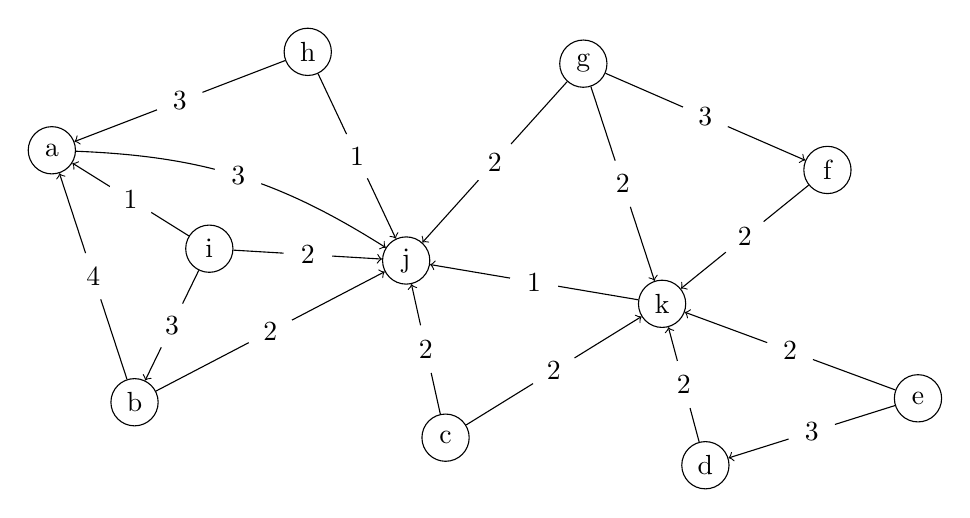
\begin{tikzpicture}
    % Nodes
    \node[circle, draw, minimum size=0.6cm, inner sep=0pt] at (0.5* 0.0, 0.5* 8.5) (a) {a};
    \node[circle, draw, minimum size=0.6cm, inner sep=0pt] at (0.5* 2.1, 0.5* 2.1) (b) {b};
    \node[circle, draw, minimum size=0.6cm, inner sep=0pt] at (0.5* 10.0, 0.5* 1.2) (c) {c};
    \node[circle, draw, minimum size=0.6cm, inner sep=0pt] at (0.5* 16.6, 0.5* 0.5) (d) {d};
    \node[circle, draw, minimum size=0.6cm, inner sep=0pt] at (0.5* 22.0, 0.5* 2.2) (e) {e};
    \node[circle, draw, minimum size=0.6cm, inner sep=0pt] at (0.5* 19.7, 0.5* 8.0) (f) {f};
    \node[circle, draw, minimum size=0.6cm, inner sep=0pt] at (0.5* 13.5, 0.5* 10.7) (g) {g};
    \node[circle, draw, minimum size=0.6cm, inner sep=0pt] at (0.5* 6.5, 0.5* 11.0) (h) {h};
    \node[circle, draw, minimum size=0.6cm, inner sep=0pt] at (0.5* 4.0, 0.5* 6.0) (i) {i};
    \node[circle, draw, minimum size=0.6cm, inner sep=0pt] at (0.5* 9.0, 0.5* 5.7) (j) {j};
    \node[circle, draw, minimum size=0.6cm, inner sep=0pt] at (0.5* 15.5, 0.5* 4.6) (k) {k};

    \draw[->] (a) edge[bend left=15] node[circle, fill=white] {3} (j);

    \draw[->] (b) edge node[circle, fill=white] {4} (a);
    \draw[->] (b) edge node[circle, fill=white] {2} (j);

    \draw[->] (c) edge node[circle, fill=white] {2} (j);
    \draw[->] (c) edge node[circle, fill=white] {2} (k);

    \draw[->] (d) edge node[circle, fill=white] {2} (k);

    \draw[->] (e) edge node[circle, fill=white] {3} (d);
    \draw[->] (e) edge node[circle, fill=white] {2} (k);

    \draw[->] (f) edge node[circle, fill=white] {2} (k);

    \draw[->] (g) edge node[circle, fill=white] {3} (f);
    \draw[->] (g) edge node[circle, fill=white] {2} (j);
    \draw[->] (g) edge node[circle, fill=white] {2} (k);

    \draw[->] (h) edge node[circle, fill=white] {3} (a);
    \draw[->] (h) edge node[circle, fill=white] {1} (j);

    \draw[->] (i) edge node[circle, fill=white] {1} (a);
    \draw[->] (i) edge node[circle, fill=white] {3} (b);
    \draw[->] (i) edge node[circle, fill=white] {2} (j);

    \draw[->] (k) edge node[circle, fill=white] {1} (j);
  \end{tikzpicture}
  \caption{Upward-Graph des Beispielgraphs}
  \label{ch::fig::upward_graph}
\end{figure}

Die Definition des Downward-Graphens erfolgt nun analog zu der des Upward-Graphens:

\begin{definition}[Downward-Graph]
  Sei $G = (V, E)$ und eine vertex-to-level-Funktion dazu gegeben. Dann ist ein Upward-Graph des transponierten Graphens $G^T$ ein \emph{Downward-Graph} zu $G$.
\end{definition}

Ist ein Graph ungerichtet, so ist er äquivalent zu seinem transponierten Graphen, daher sind dann sind auch Upward- und Downward-Graph äquivalent.
\autoref{ch::fig::upward_graph} entspricht somit gleichzeitig dem Downward-Graph des Beispielgraphens aus \autoref{graphs:fig:beispielgraph}.
Es ist zu zeigen, dass Anfragen auf einem auf diese Art definierten Contracted-Graph $C = (G_u, G_d)$ ebenfalls korrekt sind.

\begin{beweis}[Korrektheit Contracted-Graph Anfrage]
  Da sowohl im Upward- als auch im Downward-Graphen nur Kanten existieren, deren Gewicht mindestens dem kürzesten Pfad Abstand der verbundenen Knoten entspricht, kann in $C$ kein Pfad gefunden werden, der nicht auch in $G$ existiert.

  Sei ${sp}_G(s, t)$ der kürzeste $s$-$t$-Pfad auf $G$ der unter allen kürzesten $s$-$t$-Pfaden den Knoten $m$ mit dem höchsten Level enthält.
  Erstelle aus diesem Pfad $(s, \dotsc, t)$ zwei Pfade: $(s, \dotsc, m)$ und $(t, \dotsc, m)$.
  Betrachte den Teilpfad $(s, \dotsc, m)$ der Hop-Länge $n_s$.

  Finde nun den ersten Knoten $s'$ nach $s$, für den gilt, dass sein Level größer als das von $s$ ist und zwischen denen auf allen Pfaden nur Knoten kleiner Level liegen.
  Für diesen gibt es nach der Definition des Upward-Graphen eine Kante $(s, s')$ mit optimalem Gewicht.
  Wiederhole dies für den Teilpfad $(s', \dotsc, m)$, bis $s' = m$.
  Durch diese Kanten lässt sich $m$ von $s$ aus in $C$ mit optimaler Distanz finden.

  Analog wird für den Teilpfad $(t, \dotsc, m)$ im Downward-Graphen argumentiert.
  \qed
\end{beweis}

Dass nur Kanten $(t, h)$ erstellt werden müssen, wenn $h$ das größte und $t$ das zweitgrößte Level auf allen $t$-$h$-Pfaden hat, ist in \autoref{fig:people:notwendige_kanten} veranschaulicht.
Die Zahl unter dem Knotennamen entspricht dabei dem Level des Knotens.
Es muss keine $(u, w)$ Kante erstellt werden, da $w$ über $v$ erreicht werden kann.

\begin{figure}[h!]
  \centering
  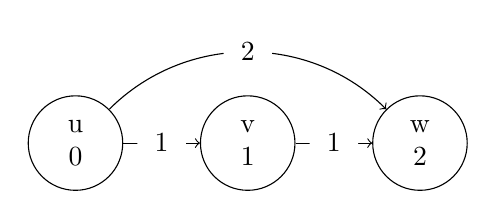
\begin{tikzpicture}[scale=1.75]
    \node[circle, draw, minimum size=1.2cm, inner sep=0pt , align=center] at (0*1.25, 0) (u) {u\\0};
    \node[circle, draw, minimum size=1.2cm, inner sep=0pt , align=center] at (1*1.25, 0) (v) {v\\1};
    \node[circle, draw, minimum size=1.2cm, inner sep=0pt , align=center] at (2*1.25, 0) (w) {w\\2};

    \draw[->] (u) edge[bend left=45] node[circle, fill=white] {2} (w);
    \draw[->] (u) edge node[circle, fill=white] {1} (v);
    \draw[->] (v) edge node[circle, fill=white] {1} (w);
  \end{tikzpicture}
  \caption{Beispiel für notwendige Kanten im Upward-Graph}
  \label{fig:people:notwendige_kanten}
\end{figure}

\subsection{Kontraktion erfüllt diese Definition}

Bei der Knoten-Kontraktion des Knotens $v$ wird für den Vorgänger-Nachfolger-Pfad $(u, v, w)$ eine Abkürzung eingefügt, wenn dies der einzige kürzeste $u$-$w$-Pfad ist.
Ist dies der Fall, dann sind die Knoten aller andern kürzesten Pfade zuvor bereits kontrahiert worden und haben ein niedrigeres Level als $u$ und $w$.
Deswegen bilden diese Abkürzungen mitsamt den Kanten des ursprünglichen Graphen die Kantenmenge des Upward- und Downward-Graphen (nach der neuen Definition \ref{people:def:upward_graph}), wobei die Zuordnung zu Downward- und Upward-Graph durch die Reihenfolge der Kontraktion von $u$ und $w$ definiert ist.

Wenn die Kontraktionsbedingung abgeschwächt wird, werden nicht notwendige und nicht optimale Kanten eingefügt, dies lässt die Definition aber zu.
Daher entspricht ein durch Graphen-Kontraktion erzeugter Graph der neuen Definition.

\subsection{Algorithmus}

Da das Berechnen aller kürzesten Pfade zwischen zwei Knoten aufwendig ist, wird die Bedingung zum Hinzufügen einer Kante bei der Berechnung eines Contracted-Graphens vereinfacht.
Es werden $(t, h)$-Kanten eingefügt, sobald ein optimaler $t$-$h$-Pfad gefunden wurde, auf dem $h$ das größte und $t$ das zweitgrößte Level hat.
Dies ist hinreichend, fügt im Zweifel jedoch mehr Kanten als notwendig ein.

Um einen Upward-Graphen zu berechnen, wird für jeden Knoten $t \in V$ eine angepasste Dijkstra-Suche ausgeführt, bei der für jeden Knoten jeweils notiert wird, was das größte Level auf dem Pfad zur Wurzel ist.
Diese Information kann mit der \emph{max-on-path} Funktion ${mop}$ abgerufen werden.
Ein Knoten $h \in V$, $h \neq t$ ist dabei der Kopf einer Upward-Graph Kante, für die ${mop}(h) = {vtl}(h)$ und ${mop}({pre}(h)) = {vtl}(t)$ gilt.
Das Gewicht der Kante wird der Dijkstra-Suche entnommen.
Die Suche kann abgebrochen werden, wenn für alle nicht-expandierten Knoten $h$ die Bedingung ${mop}({pre}(h)) > {vtl}(h)$ erfüllt ist.
Ist dies erfüllt, so hat die Wurzel $t$ auf dem $t$-$h$-Pfad nicht das zweitgrößte Level und damit kann $h$ nicht der Kopf einer Upward-Kante sein.
\autoref{ch:fig:ch_brute_force_suchbaum} zeigt dies für den Knoten $a$ im Beispielgraphen.
Die linke Zahl steht dabei für das Level des jeweiligen Knotens, die rechte Zahl für das größte Level auf dem Pfad zur Wurzel.

\begin{figure}[h!]
  \centering
  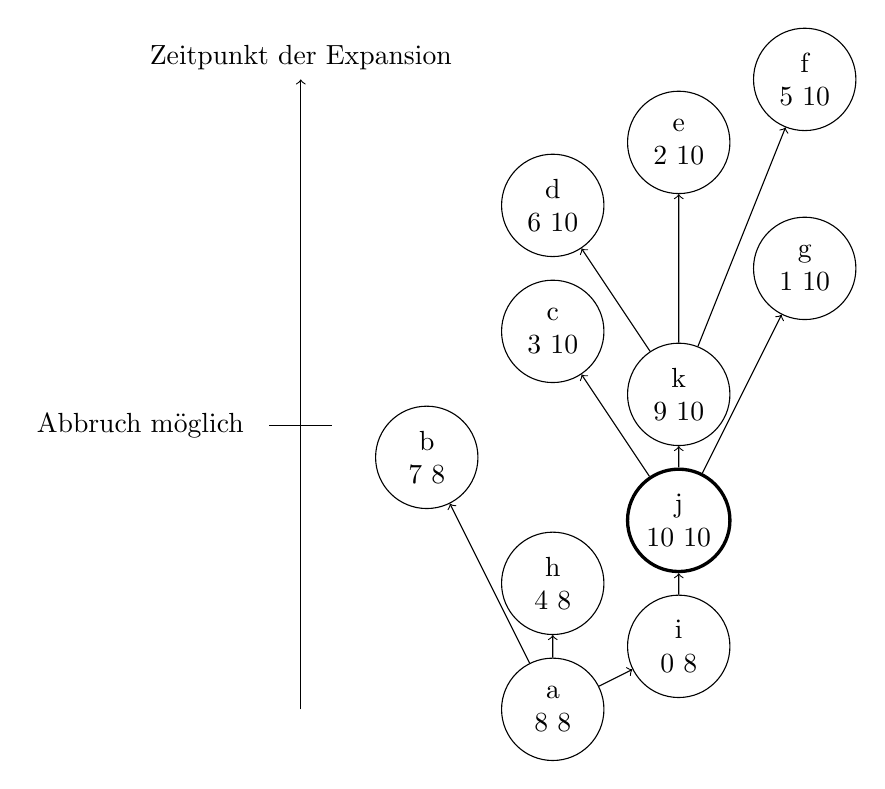
\begin{tikzpicture}[scale=0.8]
    % Nodes
    % a & b & c & d & e & f & g & h & i & j & k &
    % 8 & 7 & 3 & 6 & 2 & 5 & 1 & 4 & 0 & 10 & 9 &

    \node[circle, draw, minimum size=1.3cm, inner sep=0pt , align=center] at (2* 1, 0) (a) {a\\8 8};
    \node[circle, draw, minimum size=1.3cm, inner sep=0pt , align=center] at (2* 0, 4) (b) {b\\7 8};
    \node[circle, draw, minimum size=1.3cm, inner sep=0pt , align=center] at (2* 1, 6) (c) {c\\3 10};
    \node[circle, draw, minimum size=1.3cm, inner sep=0pt , align=center] at (2* 1, 8) (d) {d\\6 10};
    \node[circle, draw, minimum size=1.3cm, inner sep=0pt , align=center] at (2* 2, 9) (e) {e\\2 10};
    \node[circle, draw, minimum size=1.3cm, inner sep=0pt , align=center] at (2* 3, 10) (f) {f\\5 10};
    \node[circle, draw, minimum size=1.3cm, inner sep=0pt , align=center] at (2* 3, 7) (g) {g\\1 10};
    \node[circle, draw, minimum size=1.3cm, inner sep=0pt , align=center] at (2* 1, 2) (h) {h\\4 8};
    \node[circle, draw, minimum size=1.3cm, inner sep=0pt , align=center] at (2* 2, 1) (i) {i\\0 8};
    \node[circle, draw, minimum size=1.3cm, inner sep=0pt , align=center, very thick] at (2* 2, 3) (j) {j\\10 10};
    \node[circle, draw, minimum size=1.3cm, inner sep=0pt , align=center] at (2* 2, 5) (k) {k\\9 10};

    \draw[->] (a) edge (b);
    \draw[->] (a) edge (h);
    \draw[->] (a) edge (i);
    \draw[->] (j) edge (c);
    \draw[->] (i) edge (j);
    \draw[->] (k) edge (d);
    \draw[->] (j) edge (k);
    \draw[->] (k) edge (e);
    \draw[->] (k) edge (f);
    \draw[->] (j) edge (g);

    \draw[->] (-2, 0) -- (-2, 10) node[above] {Zeitpunkt der Expansion};

    \draw (-2.5, 4.5) -- (-1.5, 4.5) node[left=1cm] {Abbruch möglich};

  \end{tikzpicture}
  \caption{Contracted-Graph PEOPLE Suchbaum}
  \label{ch:fig:ch_brute_force_suchbaum}
\end{figure}

Die Information des größten Levels auf dem Pfad zur Wurzel kann dabei beim Update eines Knotens übertragen werden, indem das Maximum des bisherigen größten Levels und das Level des upgedateten Knotens gebildet wird.


Die Abbruchbedingung kann durch Betrachtung einer Menge an \emph{lebendigen Knoten} verfolgt werden.
Sobald diese keine Knoten mehr enthält, kann die Suche abgebrochen werden.
Zu Beginn ist nur der Startknoten lebendig, die Lebendigkeit wird dann jeweils an die Kinder vererbt.
Ein Knoten stirbt, nachdem er expandiert worden ist oder wenn er den Kopf einer Upward-Graph Kante bildet.
In dem Beispiel in \autoref{ch:fig:ch_brute_force_suchbaum} wäre dies etwa nach der Expansion von $b$ der Fall.
Bei einer \emph{guten} vertex-to-level-Funktion kann davon ausgegangen werden, dass viele Suchen früh abgebrochen werden können.

Die Berechnung ist \emph{embarrassingly parallel}, jeder Knoten kann unabhängig von den anderen berechnet werden.
Der textuell beschriebene Algorithmus ist im Algorithmus \ref{alg:people:ch} dargestellt und wird Contracted-Graph PEOPLE Algorithmus genannt.

\begin{algorithm}[p]
  \caption{CH-PEOPLE}
  \begin{algorithmic}[1]
    \Require Graph $G = (V, E)$, vertex-to-level Funktion ${vtl}$, Knoten $s \in V$
    \Ensure $E_s$
    \State // Initialisiere Distanz- und Vorgänger-Funktion
    \ForAll{$v \in V$}
    \State ${dist}(v) \leftarrow \infty$
    \State ${pre}(v) \leftarrow {none}$
    \EndFor

    \State
    \State // Initialisiere Suche
    \State ${dist}(s) \leftarrow 0$
    \State $Q\leftarrow \{ s \}$
    \State ${pre}(s) \leftarrow s$

    \State
    \State // Initialisiere max-on-path
    \State ${mop}(s) \leftarrow {vtl}(s)$
    \State $E_s \leftarrow \{ \}$
    \State ${alive} \leftarrow \{ s \}$

    \State
    \While{$Q \neq \emptyset \land {alive} \neq \emptyset$}
    \State $u \leftarrow{extract\_min}(Q)$\label{graphs:dijkstra:pop}

    \State
    \State // Baue Kantenmenge
    \If {$u \neq s \land {mop}(u) = {vtl}(u)$}
    \State $E_s \leftarrow E_s \cup \{ (s, u, {dist}(u)) \}$
    \State ${alive} \leftarrow {alive} \setminus \{ u \}$
    \EndIf

    \State
    \State // Aktualisiere Nachbarn
    \ForAll{$(u, v, w) \in E$}
    \If {${dist}(u) + w < {dist}(v)$}
    \State ${dist}(v) \leftarrow {dist}(u) + w$
    \State ${pre}(u) \leftarrow v$
    \State $Q = Q \cup \{ v \}$
    \State
    \State // setze max\_level\_path
    \State ${mop}(v) \leftarrow \max({mop}(v), {vtl}(v))$
    \State
    \If {$u \in {alive}$}
    \State ${alive} \leftarrow {alive} \cup \{ v \}$
    \EndIf
    \EndIf
    \EndFor

    \State ${alive} \leftarrow {alive} \setminus \{ u \}$

    \EndWhile

    \State
    \State \Return $E_s$
  \end{algorithmic}
  \label{alg:people:ch}
\end{algorithm}

\subsection{Änderung von Kantengewichten}

Bei Graphen mit hierarchischer Struktur und einer guten vertex-to-Level-Funktion ist anzunehmen, dass die Suche nach Algorithmus \ref{alg:people:ch}  in den meisten Fällen früh abbricht.
Dies ist einerseits für die Effizienz der Berechnung von Vorteil, verdeutlicht aber auch, dass für die Bestimmung der ausgehenden Kanten des Contracted-Graphen für viele Knoten jeweils nur ihre lokale Umgebung von Bedeutung ist, wobei insbesondere Knoten mit einem hohen Level hierbei eine Ausnahme bilden.
Änderungen der Kantengewichte außerhalb dieser Umgebung haben daher für viele Knoten keinen Einfluss auf den Suchbaum des Algorithmus \ref{alg:people:ch}.

Diese Eigenschaft lässt sich nutzen, um nach einer Änderung der Kantengewichte nicht für jeden Knoten sämtliche ausgehenden Kanten neu berechnen zu müssen.
Zwei mögliche Ansätze bieten sich hierfür an:
Zum einen könnte für jeden Knoten gespeichert werden, von welchen Kanten er beeinflusst wird.
Zum anderen könnte für eine geänderte Kante berechnet werden, welche Knoten von ihr beeinflusst werden.

Das Speichern des Bereichs, der einen Knoten beeinflusst, kann in Graphen in der euklidischen Ebene beispielsweise durch Bounding-Boxen realisiert werden.
Ob es eine effiziente Methode gibt, mit der der Einflussbereich einer Kante bestimmt werden kann, wird in dieser Arbeit nicht behandelt.

\subsection{Abkürzungsproblem}

Es liegt nahe, als abgekürzten Knoten denjenigen Knoten mit dem dritthöchsten Level auszuwählen und sich darauf zu verlassen, dass die Suche von diesem aus die nächste Abkürzung findet, da dies der Knoten-Kontraktion entspricht.
Das ist praktisch, da dann jede Abkürzung nur einmal erstellt werden muss, dafür muss jedoch gelten, dass die Vorwärtssuche für $s$-$t$ den gleichen Pfad findet wie die Rückwärtssuche (die Suche auf dem transponierten Graphen) für $t$-$s$.
Dies ist nicht garantiert, wenn als Graph eine Datenstruktur verwendet wird, welche die Nachbarn nicht in einer definierten Ordnung ausgibt (etwa eine HashMap).
Eine nicht stabile Prioritätswarteschlange hat ebenfalls den gleichen Effekt.

\autoref{ch:fig:problem_shortcut} zeigt ein solches Szenario.
Im Contracted-Graphen $C$ wurde der $a$-$e$-Pfad $(a, e)$ gefunden, dessen Abkürzungen nun ersetzt werden.
Zunächst wird für die Abkürzung $(a, e)$ der abgekürzte Knoten $d$ gefunden, was zu dem Pfad $(a, d, e)$ führt.
Es wird darauf vertraut, dass die Suche von $d$ aus die Abkürzung $(d, a)$ mit dem Knoten $b$ findet, jedoch geschieht dies nicht, wenn $a$ von $d$ aus über $c$ erreicht wird.

\begin{figure}[h!]
  \centering
  \begin{subfigure}[b]{0.49\textwidth}
    \centering
    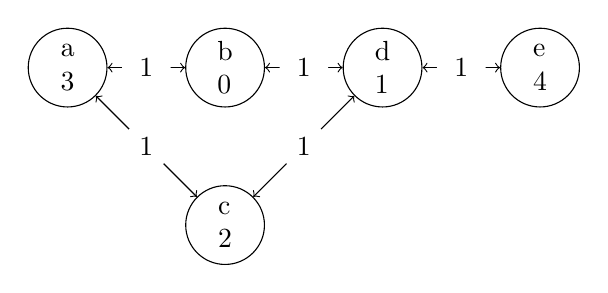
\begin{tikzpicture}
      % Nodes
      \node[circle, draw, minimum size=1cm, inner sep=0pt, align=left] at (2*0, 2*0) (a) {a\\3};
      \node[circle, draw, minimum size=1cm, inner sep=0pt, align=left] at (2*1, 2*0) (b) {b\\0};
      \node[circle, draw, minimum size=1cm, inner sep=0pt, align=left] at (2*1, 2*-1) (c) {c\\2};
      \node[circle, draw, minimum size=1cm, inner sep=0pt, align=left] at (2*2, 2*0) (d) {d\\1};
      \node[circle, draw, minimum size=1cm, inner sep=0pt, align=left] at (2*3, 2*0) (e) {e\\4};

      \draw[<->] (a) edge node[circle, fill=white] {1} (b);
      \draw[<->] (b) edge node[circle, fill=white] {1} (d);
      \draw[<->] (d) edge node[circle, fill=white] {1} (e);

      \draw[<->] (a) edge node[circle, fill=white] {1} (c);
      \draw[<->] (c) edge node[circle, fill=white] {1} (d);
    \end{tikzpicture}
    \caption{Graph}
  \end{subfigure}
  \hfill
  \begin{subfigure}[b]{0.49\textwidth}
    \centering
    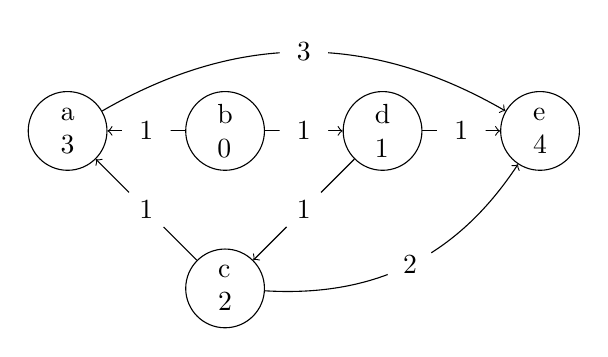
\begin{tikzpicture}
      % Nodes
      \node[circle, draw, minimum size=1cm, inner sep=0pt, align=left] at (2*0, 2*0) (a) {a\\3};
      \node[circle, draw, minimum size=1cm, inner sep=0pt, align=left] at (2*1, 2*0) (b) {b\\0};
      \node[circle, draw, minimum size=1cm, inner sep=0pt, align=left] at (2*1, 2*-1) (c) {c\\2};
      \node[circle, draw, minimum size=1cm, inner sep=0pt, align=left] at (2*2, 2*0) (d) {d\\1};
      \node[circle, draw, minimum size=1cm, inner sep=0pt, align=left] at (2*3, 2*0) (e) {e\\4};

      \draw[<-] (a) edge node[circle, fill=white] {1} (b);
      \draw[->] (b) edge node[circle, fill=white] {1} (d);
      \draw[->] (d) edge node[circle, fill=white] {1} (e);

      \draw[->] (c) edge node[circle, fill=white] {1} (a);
      \draw[<-] (c) edge node[circle, fill=white] {1} (d);

      \draw[->] (c) edge[bend right] node[circle, fill=white] {2} (e);
      \draw[->] (a) edge[bend left] node[circle, fill=white] {3} (e);
    \end{tikzpicture}
    \caption{Upward- und Downard-Graph von $C$}
  \end{subfigure}
  \begin{subfigure}[b]{0.49\textwidth}
    \centering
    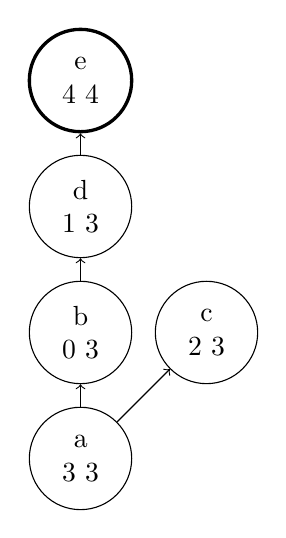
\begin{tikzpicture}[scale=0.8]
      % Nodes
      \node[circle, draw, minimum size=1.3cm, inner sep=0pt, align=center] at (2*0, 2*0) (a) {a\\3 3};
      \node[circle, draw, minimum size=1.3cm, inner sep=0pt, align=center] at (2*0, 2*1) (b) {b\\0 3};
      \node[circle, draw, minimum size=1.3cm, inner sep=0pt, align=center] at (2*1, 2*1) (c) {c\\2 3};
      \node[circle, draw, minimum size=1.3cm, inner sep=0pt, align=center] at (2*0, 2*2) (d) {d\\1 3};
      \node[circle, draw, minimum size=1.3cm, inner sep=0pt, align=center, very thick] at (2*0, 2*3) (e) {e\\4 4};

      \draw[->] (a) edge node[] {} (b);
      \draw[->] (b) edge node[] {} (d);
      \draw[->] (d) edge node[] {} (e);
      \draw[->] (a) edge node[] {} (c);
    \end{tikzpicture}
    \caption{Suchbaum von $a$}
  \end{subfigure}
  \hfill
  \begin{subfigure}[b]{0.49\textwidth}
    \centering
    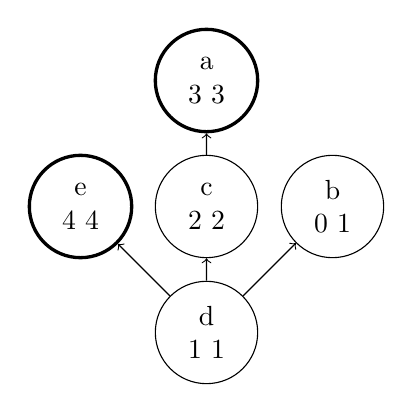
\begin{tikzpicture}[scale=0.8]
      % Nodes
      \node[circle, draw, minimum size=1.3cm, inner sep=0pt, align=center, very thick] at (2*1, 2*2) (a) {a\\3 3};
      \node[circle, draw, minimum size=1.3cm, inner sep=0pt, align=center] at (2*2, 2*1) (b) {b\\0 1};
      \node[circle, draw, minimum size=1.3cm, inner sep=0pt, align=center] at (2*1, 2*1) (c) {c\\2 2};
      \node[circle, draw, minimum size=1.3cm, inner sep=0pt, align=center] at (2*1, 2*0) (d) {d\\1 1};
      \node[circle, draw, minimum size=1.3cm, inner sep=0pt, align=center, very thick] at (2*0, 2*1) (e) {e\\4 4};

      \draw[->] (d) edge node[] {} (e);
      \draw[->] (d) edge node[] {} (c);
      \draw[->] (d) edge node[] {} (b);
      \draw[->] (c) edge node[] {} (a);
    \end{tikzpicture}
    \caption{Suchbaum von $d$}
  \end{subfigure}
  \caption{Problem beim Shortcut erstellen}
  \label{ch:fig:problem_shortcut}
\end{figure}

Für dieses Problem gibt es zwei Lösungen:
Für jede Abkürzung $(t, h)$ werden alle weiteren Abkürzungen die benötigt werden, um aus $(t, h)$ einen Pfad auf $G$ zu erstellen, gesammelt.
Dadurch werden viele Abkürzungen mehrfach erstellt, da eine Abkürzung Teil einer anderen Abkürzung sein kann.
Dies muss daher zwischen den einzelnen CH-PEOPLE Suchen synchronisiert werden, um den Speicherverbrauch zu minimieren.

Alternativ kann die Prioritätswarteschlange modifiziert werden, indem eine Totalordnung der Knoten bestimmt, in welcher Reihenfolge Knoten gleicher Distanz expandiert werden.

\section{PEOPLE}

Analog zur neuen Definition des Contracted-Graph lässt sich auch der Hub-Graph neu definieren.
Die dafür verwendete Definition des Forward-Labels weicht nur leicht von der des Upward-Graphen ab, lediglich die Anforderung, dass der Fuß einer Kante das zweitgrößte Level hat, entfällt.

\begin{definition}[Forward-Label]
  Sei $G = (V, E)$ und eine vertex-to-level Funktion dazu gegeben.
  Dann ist $L_f (t) \subset V \times \mathbb{R}$ ein Forward-Label für einen Knoten $t$ in $G$, wenn gilt:

  \begin{itemize}
    \item
          $L_f (t)$ enthält nur Einträge $(h, d)$ mit $h \in V$ und $d \in \mathbb{R}$, für die es einen $t$-$h$ Pfad der Länge $d \geq {spd}_G (t, h)$ gibt, sodass auf ihm $h$ das größte Level hat.

    \item
          $L_f (t)$ enthält alle Einträge $(h, {spd}_G (t, h))$ mit $h \in V$, für die gilt, dass auf \emph{allen} $t$-$h$ Pfaden $h$ das größte Level hat.
  \end{itemize}
\end{definition}


Hierbei ist ein Backward-Label ein Forward-Label des transponierten Graphen $G^T$.
Die Korrektheit dieser Definition folgt direkt daraus, dass der Knoten mit dem höchsten Level auf einem Pfad im Forward- und Backward-Label liegt.

\subsection{Algorithmus}

Solche Labels können wieder durch Merging aus einem Contracted-Graph erstellt werden, jedoch folgt aus dieser Definition auch die Möglichkeit, das Label eines bestimmten Knotens zu berechnen.
Der dafür verwendete Algorithmus ist in Algorithmus \ref{alg:people:people} gelistet, er erzeugt ein gepruntes Label, da er aus einem Dijkstra-Suchbaum auf $G$ das Label erzeugt und dieser nur optimale Distanzen enthält.
Da er für eine vorgegebene vertex-to-level-Funktion geprunte Label liefert, wird dieser Algorithmus PEOPLE, für \textbf{P}r\textbf{E}determined \textbf{O}rder, \textbf{P}runed \textbf{L}ab\textbf{e}l, genannt.

Ein Beispiel einer solchen Suche ist in \autoref{ch:fig:hl_brute_force_suchbaum} gezeichnet.
Das Label für $a$ enthält $j$, $f$ und $a$ selbst, da ihr Level das jeweils größte auf dem Pfad zur Wurzel ist.

\begin{figure}[h!]
  \centering
  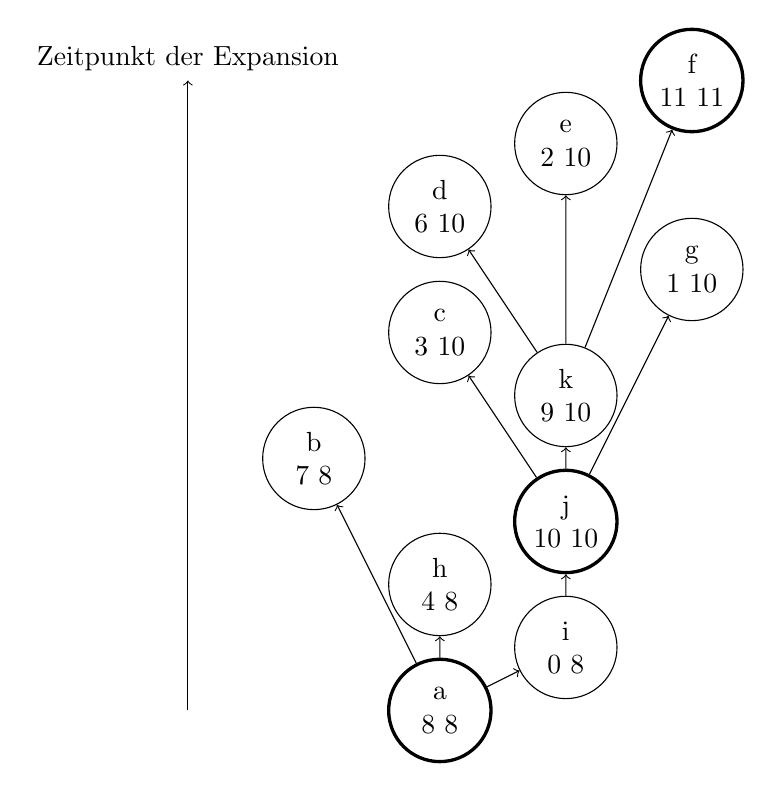
\begin{tikzpicture}[scale=0.8]
    % Nodes
    % a & b & c & d & e & f & g & h & i & j & k &
    % 8 & 7 & 3 & 6 & 2 & 5 & 1 & 4 & 0 & 10 & 9 &

    \node[circle, draw, minimum size=1.3cm, inner sep=0pt , align=center, very thick] at (2* 1, 0) (a) {a\\8 8};
    \node[circle, draw, minimum size=1.3cm, inner sep=0pt , align=center] at (2* 0, 4) (b) {b\\7 8};
    \node[circle, draw, minimum size=1.3cm, inner sep=0pt , align=center] at (2* 1, 6) (c) {c\\3 10};
    \node[circle, draw, minimum size=1.3cm, inner sep=0pt , align=center] at (2* 1, 8) (d) {d\\6 10};
    \node[circle, draw, minimum size=1.3cm, inner sep=0pt , align=center] at (2* 2, 9) (e) {e\\2 10};
    \node[circle, draw, minimum size=1.3cm, inner sep=0pt , align=center, very thick] at (2* 3, 10) (f) {f\\11 11};
    \node[circle, draw, minimum size=1.3cm, inner sep=0pt , align=center] at (2* 3, 7) (g) {g\\1 10};
    \node[circle, draw, minimum size=1.3cm, inner sep=0pt , align=center] at (2* 1, 2) (h) {h\\4 8};
    \node[circle, draw, minimum size=1.3cm, inner sep=0pt , align=center] at (2* 2, 1) (i) {i\\0 8};
    \node[circle, draw, minimum size=1.3cm, inner sep=0pt , align=center, very thick] at (2* 2, 3) (j) {j\\10 10};
    \node[circle, draw, minimum size=1.3cm, inner sep=0pt , align=center] at (2* 2, 5) (k) {k\\9 10};

    \draw[->] (a) edge (b);
    \draw[->] (a) edge (h);
    \draw[->] (a) edge (i);
    \draw[->] (j) edge (c);
    \draw[->] (i) edge (j);
    \draw[->] (k) edge (d);
    \draw[->] (j) edge (k);
    \draw[->] (k) edge (e);
    \draw[->] (k) edge (f);
    \draw[->] (j) edge (g);

    \draw[->] (-2, 0) -- (-2, 10) node[above] {Zeitpunkt der Expansion};

  \end{tikzpicture}
  \caption{Hub-Graph PEOPLE Suchbaum}
  \label{ch:fig:hl_brute_force_suchbaum}
\end{figure}

\begin{algorithm}[p]
  \caption{PEOPLE}
  \begin{algorithmic}[1]
    \Require Graph $G = (V, E)$, vertex-to-level Funktion ${vtl}$, Knoten $s \in V$
    \Ensure $L_f (s)$
    \State // Initialisiere Distanz- und Vorgänger-Funktion
    \ForAll{$v \in V$}
    \State ${dist}(v) \leftarrow \infty$
    \State ${pre}(v) \leftarrow {none}$
    \EndFor

    \State
    \State // Initialisiere Suche
    \State ${dist}(s) \leftarrow 0$
    \State $Q\leftarrow \{ s \}$
    \State ${pre}(s) \leftarrow s$

    \State
    \State // Initialisiere max-on-path
    \State ${mop}(s) \leftarrow {vtl}(s)$
    \State $L_f (s) \leftarrow \{ \}$

    \State
    \While{$Q \neq \emptyset$}
    \State $u \leftarrow{extract\_min}(Q)$

    \State
    \State // Baue Label
    \If {${mop}(u) = {vtl}(u)$}
    \State $L_f (s) \leftarrow L_f (s) \cup \{ (u, {dist}(u)) \}$
    \EndIf

    \State
    \State // Aktualisiere Nachbarn
    \ForAll{$(u, v, w) \in E$}
    \If {${dist}(u) + w < {dist}(v)$}
    \State ${dist}(v) \leftarrow {dist}(u) + w$
    \State ${pre}(u) \leftarrow v$
    \State $Q = Q \cup \{ v \}$
    \State
    \State // setze max\_level\_path
    \State ${mop}(v) \leftarrow \max({mop}(v), {vtl}(v))$
    \EndIf
    \EndFor

    \EndWhile

    \State
    \State \Return $L_f (s)$
  \end{algorithmic}
  \label{alg:people:people}
\end{algorithm}

\subsection{Größe der Label}\label{subsection:people:label_size}

Die mit PEOPLE erzeugten Labels können mitunter kleiner sein, als durch Merging erzeugte Label.
Insbesondere kann das Merging von Contracted-Graphen, welche durch Graphen-Kontraktion erzeugt wurden, Labels erzeugen, die nicht minimal sind.

\autoref{fig:people:better_label_size} zeigt ein solches Beispiel, wobei die Zahl unter dem Namen des Knotens dem Level des Knotens entspricht.
Der Upward-Graph kann hierbei sowohl durch PEOPLE als auch durch Graphen-Kontraktion erstellt worden sein.
Nach der neuen Definition des Forward-Labels muss das Label von $c$ nur $d$ und $b$ enthalten.
Wird es aber durch Merging erzeugt, so enthält es auch $a$.
Dieses Verhalten tritt auf, wenn kürzeste Pfaden nicht eindeutig sind, daher ist anzunehmen, dass unter anderem in Grid-Graphen dieses Phänomen häufiger auftritt.

Um tatsächlich minimale Label zu erzeugen, muss der Algorithmus \ref{alg:people:people} verändert werden:
Kann ein Knoten $v$ über $u$ erreicht werden, aber die Kosten hierfür sind gleich groß wie bisher, so wird $u$ trotzdem als Vorgänger von $v$ gesetzt, wenn ${mop}(u) > {mop}(v)$.

\begin{figure}[h!]
  \begin{subfigure}[b]{0.49\textwidth}
    \centering
    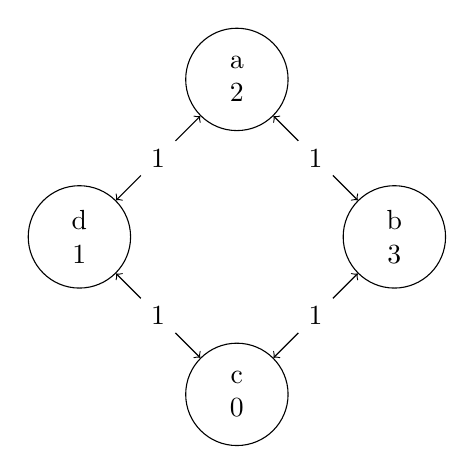
\begin{tikzpicture}[scale=1]
      % Nodes
      \node[circle, draw, minimum size=1.3cm, inner sep=0pt, align=center] at (2*1, 2*2) (a) {a\\2};
      \node[circle, draw, minimum size=1.3cm, inner sep=0pt, align=center] at (2*2, 2*1) (b) {b\\3};
      \node[circle, draw, minimum size=1.3cm, inner sep=0pt, align=center] at (2*1, 2*0) (c) {c\\0};
      \node[circle, draw, minimum size=1.3cm, inner sep=0pt, align=center] at (2*0, 2*1) (d) {d\\1};

      \draw[<->] (a) edge node[circle, fill=white] {1} (b);
      \draw[<->] (b) edge node[circle, fill=white] {1} (c);
      \draw[<->] (c) edge node[circle, fill=white] {1} (d);
      \draw[<->] (d) edge node[circle, fill=white] {1} (a);
    \end{tikzpicture}
    \caption{Graph}
  \end{subfigure}
  \hfill
  \begin{subfigure}[b]{0.49\textwidth}
    \centering
    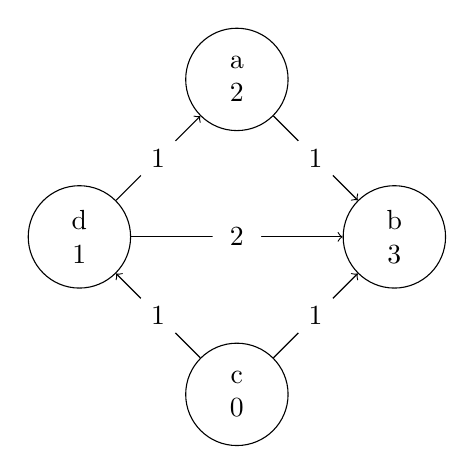
\begin{tikzpicture}[scale=1]
      % Nodes
      \node[circle, draw, minimum size=1.3cm, inner sep=0pt, align=center] at (2*1, 2*2) (a) {a\\2};
      \node[circle, draw, minimum size=1.3cm, inner sep=0pt, align=center] at (2*2, 2*1) (b) {b\\3};
      \node[circle, draw, minimum size=1.3cm, inner sep=0pt, align=center] at (2*1, 2*0) (c) {c\\0};
      \node[circle, draw, minimum size=1.3cm, inner sep=0pt, align=center] at (2*0, 2*1) (d) {d\\1};


      \draw[->] (c) edge node[circle, fill=white] {1} (d);
      \draw[->] (c) edge node[circle, fill=white] {1} (b);

      \draw[->] (d) edge node[circle, fill=white] {2} (b);
      \draw[->] (d) edge node[circle, fill=white] {1} (a);

      \draw[->] (a) edge node[circle, fill=white] {1} (b);
    \end{tikzpicture}
    \caption{Upward- und Downward-Graph}
  \end{subfigure}
  \caption{Beispiel für nicht-minimale Label}



  \label{fig:people:better_label_size}
\end{figure}

\subsection{Anwendungsgebiet}

Die Berechnung der Graphen-Kontraktion in Straßennetzwerken ist in vertretbarer Zeit möglich, jedoch gilt dies nicht für alle Graphklassen.
Insbesondere bei Graphen mit hohem durchschnittlichen Knotengrad stellt die Dijkstra-Suche für jeden Vorgänger einen signifikanten Kostenfaktor dar, sodass die Berechnung der Labels mittels PEOPLE effizienter sein kann.
Da die Labels parallel berechnet werden können, ist es durch den Einsatz geeigneter Hardware möglich, die Berechnungszeit zu verkürzen.

Der Algorithmus kann auch dazu verwendet werden, die Ergebnisse einer $s$-$t$-Anfrage effizient zu cachen.
Falls die Labels von $s$ und $t$ noch nicht vorhanden sind, werden sie generiert.
Nachfolgende Anfragen von $s$ oder nach $t$ können dann direkt auf die gespeicherten Labels zugreifen.

PEOPLE kann auch dafür benutzt werden, die durch eine vertex-to-level-Funktion induzierte durchschnittliche Label Größe anzugeben, ohne zuerst den Contracted-Graph und anschließend den Hub-Graphen zu berechnen.
Hierfür wird für $n \in \mathbb{N}$ Knoten das Label berechnet und über diese die durchschnittliche Größe der Labels angegeben.
Da sich dies leicht parallelisieren lässt, könnte in einem zukünftigen Schritt durch Optimierungsalgorithmen die Labelgrößen verkleinert werden.
\chapter{Ergebnisse}

Sofern nicht anders erwähnt, beziehen sich die Laufzeiten auf Systeme mit zwei Intel Xeon Gold 6230 Prozessoren mit einer Taktrate von \SI{2.1}{\giga\hertz} und \SI{180}{\giga\byte} RAM.
Die Ergebnisse wurden auf verschiedenen, aber identisch ausgestatteten Systemen des BwUniCluster2.0 erzeugt.

\section{Untersuchung der Graphen}

Der Fokus dieser Arbeit liegt auf drei Sichtbarkeitsgraphen, die jeweils einen Ausschnitt der Ozeane repräsentieren.
Ihre Knoten liegen dabei auf den Küsten.
Für jeden dieser drei Sichtbarkeitsgraphen existiert zusätzlich eine Triangulierung, deren Abstände eine obere Schranke zu den Abständen der jeweiligen Sichtbarkeitsgraphen darstellen.
\autoref{table:input_graphs} listet die Anzahl der Kanten und Knoten der Graphen auf.
Die Graphen mit dem Präfix \emph{aegaeis} umfassen das Ägäische Meer, diejenigen mit \emph{medi} decken das Mittelmeer ab, und die mit \emph{pata} repräsentieren die Chilenischen Fjorde.
Graphen mit dem Suffix \emph{visibility} sind Sichtbarkeitsgraphen, mit \emph{graph} Triangulierungen.

Die untersuchten Graphen sind ungerichtet, werden jedoch im weiteren Verlauf dieser Arbeit als gerichtet betrachtet.
Insbesondere ist die in \autoref{table:input_graphs} aufgelistete Anzahl an Kanten gerichtet zu interpretieren, die ungerichtete Kante $\{a, b\}$ wird also doppelt gezählt als $(a, b)$ und $(b, a)$.

\begin{table}[h!]
  \centering
  \begin{tabular}{
      l % Graph
      S[table-format = 7.0] % Zeit
      S[table-format = 9.0] % Zeit
      S[table-format = 4.1] % Zeit
    }
    \toprule
    {Graph}            & {\# Knoten} & {\# Kanten} & {$\varnothing$ Grad}       \\ \midrule
    aegaeis-graph      & 524881      & 2795322     & \fpeval{2795322/524881}    \\
    aegaeis-visibility & 201040      & 310231834   & \fpeval{310231834/201040}  \\
    medi-graph         & 795606      & 4223566     & \fpeval{4223566/795606}    \\
    medi-visibility    & 310116      & 730772548   & \fpeval{730772548/310116}  \\
    pata-graph         & 2240339     & 11632900    & \fpeval{11632900/2240339}  \\
    pata-visibility    & 1002235     & 315653892   & \fpeval{315653892/1002235} \\ \bottomrule
  \end{tabular}
  \caption{Bearbeitete Graphen}
  \label{table:input_graphs}
\end{table}

\subsection{Dijkstra}

Für die Berechnung des Speedups der angewendeten Methoden wurden für jeden Graphen \num{1000} sequentielle $s$-$t$-Dijkstra-Suchen ausgeführt und die durchschnittliche Laufzeit ermittelt.
Die ermittelten Zeiten für das Finden des $s$-$t$-Abstands sind in Tabelle \ref{fig:ergebnisse:dijkstra} dargestellt.
Aus den Ergebnissen geht hervor, dass die Dijkstra-Suchen auf den Sichtbarkeitsgraphen im Vergleich zu auf ihren Triangulierungen deutlich höhere Laufzeiten aufweisen.

Zusätzlich zur durchschnittlichen Dijkstra-Laufzeit wurden die Durchschnittswerte der Hop-Längen, des Dijkstra-Ranks und der Queue-Pops über \num{10000} parallele $s$-$t$-Dijkstra-Suchen ermittelt, um ein Verständnis für die Laufzeiten zu erlangen.
Der Dijkstra-Rank ist die Anzahl der expandierten Knoten zum Zeitpunkt der Expansion des Zielknotens, die Queue-Pops die Anzahl der aus der Prioritätswarteschlange der Dijkstra-Suche entnommen Knoten.
Es zeigte sich, dass die durchschnittliche Hop-Länge in den Sichtbarkeitsgraphen signifikant kürzer ist als in den Triangulierungen.
Obwohl die Sichtbarkeitsgraphen weniger Knoten aufweisen, ist die durchschnittliche Anzahl der Queue-Pops dennoch höher.

\begin{table}[h!]
  \centering
  \begin{tabular}{
      l % Graph
      S[table-format = 4.1] % Zeit
      S[table-format = 3.0] % hop-länge
      S[table-format = 7.0] % rank
      S[table-format = 7.0] % queue pops
    }
    \toprule
    {Graph}            & {$\varnothing$ $t({spd})$} & {$\varnothing$  Hop-Länge} & {$\varnothing$ Dijkstra-Rank} & {$\varnothing$ Queue-Pops} \\
                       & {(\si{\ms})}               &                            &                               &                            \\
    \midrule
    aegaeis-graph      & 60.281198                  & 215.7201                   & 260447.36                     & 325845.56                  \\
    aegaeis-visibility & 630.434928                 & 16.311                     & 98650.82                      & 517346.63                  \\
    medi-graph         & 87.08376                   & 340.445                    & 394855.78                     & 494553.97                  \\
    medi-visibility    & 1279.67479                 & 23.6149                    & 154092.42                     & 959206.4                   \\
    pata-graph         & 265.825771                 & 883.979                    & 1120841.9                     & 1387047.8                  \\
    pata-visibility    & 1017.695977                & 63.817                     & 498570.2                      & 2429689.8                  \\ \bottomrule
  \end{tabular}
  \caption{Kennwerte der Dijkstra-Suchen}
  \label{fig:ergebnisse:dijkstra}
\end{table}

\subsection{Knotengrade}

Es wurde die Verteilung der Knotengrade untersucht, die resultierenden Histogramme sind in \autoref{ergebnisse:fig:degree_hist} dargestellt.
Als Indikator dafür, wie stark sich die Graphen kontrahieren lassen, wurde die Summe der quadratischen Knotengrade berechnet, diese sind in \autoref{table:sum_quad_degree} aufgelistet.
Bei den Sichtbarkeitsgraphen ist die Summe jeweils um mehrere Größenordnungen größer als bei ihren Triangulierungen, was darauf hindeutet, dass die Kontraktion dieser Graphen deutlich rechenintensiver sein dürfte.

\begin{figure}[p]
  \begin{subfigure}[b]{0.5\textwidth}
    \resizebox{\textwidth}{!}{%
      \begin{tikzpicture}
        \begin{axis}[
            tick align=outside,
            tick pos=left,
            xmin=-698, xmax=14702,
            xtick style={color=black},
            xtick distance=2000,
            ymin=0, ymax=0.747618384401001,
            ytick style={color=black},
            ytick={0,0.1,0.2,0.3,0.4,0.5,0.6,0.7,0.8},
            yticklabels={0,10,20,30,40,50,60,70,80},
            xlabel={Knotengrad},
            ylabel={Anteil der Knoten (\%)}
          ]
          \draw[pattern=north east lines, pattern color=CadetBlue] (axis cs:2,0) rectangle (axis cs:2002,0.712017508953334);
          \draw[pattern=north east lines, pattern color=CadetBlue] (axis cs:2002,0) rectangle (axis cs:4002,0.194220055711032);
          \draw[pattern=north east lines, pattern color=CadetBlue] (axis cs:4002,0) rectangle (axis cs:6002,0.0606247512935969);
          \draw[pattern=north east lines, pattern color=CadetBlue] (axis cs:6002,0) rectangle (axis cs:8002,0.0205382013530728);
          \draw[pattern=north east lines, pattern color=CadetBlue] (axis cs:8002,0) rectangle (axis cs:10002,0.00766514126545947);
          \draw[pattern=north east lines, pattern color=CadetBlue] (axis cs:10002,0) rectangle (axis cs:12002,0.00397930760049903);
          \draw[pattern=north east lines, pattern color=CadetBlue] (axis cs:12002,0) rectangle (axis cs:14002,0.000955033824119655);
        \end{axis}
      \end{tikzpicture}
    }
    \caption{aegaeis-visibility}
  \end{subfigure}%
  \begin{subfigure}[b]{0.5\textwidth}
    \resizebox{\textwidth}{!}{%
      \begin{tikzpicture}
        \begin{axis}[
            tick align=outside,
            tick pos=left,
            xlabel={Knotengrad},
            xmin=-1198, xmax=25202,
            xtick distance=4000,
            xtick style={color=black},
            ylabel={Anteil der Knoten (\%)},
            ymin=0, ymax=0.637890337808629,
            ytick style={color=black},
            ytick={0,0.1,0.2,0.3,0.4,0.5,0.6,0.7},
            yticklabels={0,10,20,30,40,50,60,70}
          ]
          \draw[pattern=north east lines, pattern color=CadetBlue] (axis cs:2,0) rectangle (axis cs:2002,0.60751460743679);
          \draw[pattern=north east lines, pattern color=CadetBlue] (axis cs:2002,0) rectangle (axis cs:4002,0.207212784893063);
          \draw[pattern=north east lines, pattern color=CadetBlue] (axis cs:4002,0) rectangle (axis cs:6002,0.0905080679486225);
          \draw[pattern=north east lines, pattern color=CadetBlue] (axis cs:6002,0) rectangle (axis cs:8002,0.0423164235317719);
          \draw[pattern=north east lines, pattern color=CadetBlue] (axis cs:8002,0) rectangle (axis cs:10002,0.0196700589456533);
          \draw[pattern=north east lines, pattern color=CadetBlue] (axis cs:10002,0) rectangle (axis cs:12002,0.0103219440467273);
          \draw[pattern=north east lines, pattern color=CadetBlue] (axis cs:12002,0) rectangle (axis cs:14002,0.00818403436132265);
          \draw[pattern=north east lines, pattern color=CadetBlue] (axis cs:14002,0) rectangle (axis cs:16002,0.00425647177184629);
          \draw[pattern=north east lines, pattern color=CadetBlue] (axis cs:16002,0) rectangle (axis cs:18002,0.00420165357478464);
          \draw[pattern=north east lines, pattern color=CadetBlue] (axis cs:18002,0) rectangle (axis cs:20002,0.00342452501643997);
          \draw[pattern=north east lines, pattern color=CadetBlue] (axis cs:20002,0) rectangle (axis cs:22002,0.00236363167330556);
          \draw[pattern=north east lines, pattern color=CadetBlue] (axis cs:22002,0) rectangle (axis cs:24002,2.57967986172503e-05);
        \end{axis}
      \end{tikzpicture}%
    }%
    \caption{medi-visibility}%
  \end{subfigure}%
  \par\bigskip\bigskip
  \begin{subfigure}[b]{0.5\textwidth}%
    \resizebox{\textwidth}{!}{%
      \begin{tikzpicture}%
        \begin{axis}[
            tick align=outside,
            tick pos=left,
            xlabel={Knotengrad},
            ylabel={Anteil der Knoten (\%)},
            xmin=-998, xmax=21002,
            xtick style={color=black},
            y grid style={darkgray176},
            xtick distance=4000,
            ymin=0, ymax=1.02857224104146,
            ytick style={color=black},
            ytick={0,0.2,0.4,0.6,0.8,1,1.2},
            yticklabels={0,20,40,60,80,100,120}
          ]
          \draw[pattern=north east lines, pattern color=CadetBlue] (axis cs:2,0) rectangle (axis cs:2002,0.979592610515676);
          \draw[pattern=north east lines, pattern color=CadetBlue] (axis cs:2002,0) rectangle (axis cs:4002,0.0169022235303201);
          \draw[pattern=north east lines, pattern color=CadetBlue] (axis cs:4002,0) rectangle (axis cs:6002,0.00222602483448042);
          \draw[pattern=north east lines, pattern color=CadetBlue] (axis cs:6002,0) rectangle (axis cs:8002,0.000968834654540784);
          \draw[pattern=north east lines, pattern color=CadetBlue] (axis cs:8002,0) rectangle (axis cs:10002,0.000297335455255565);
          \draw[pattern=north east lines, pattern color=CadetBlue] (axis cs:10002,0) rectangle (axis cs:12002,3.99107993631631e-06);
          \draw[pattern=north east lines, pattern color=CadetBlue] (axis cs:12002,0) rectangle (axis cs:14002,0);
          \draw[pattern=north east lines, pattern color=CadetBlue] (axis cs:14002,0) rectangle (axis cs:16002,9.97769984079078e-07);
          \draw[pattern=north east lines, pattern color=CadetBlue] (axis cs:16002,0) rectangle (axis cs:18002,3.99107993642733e-06);
          \draw[pattern=north east lines, pattern color=CadetBlue] (axis cs:18002,0) rectangle (axis cs:20002,3.99107993631631e-06);
        \end{axis}

      \end{tikzpicture}
    }
    \caption{pata-visibility}
  \end{subfigure}
  \caption{Verteilung der Kantengrade}
  \label{ergebnisse:fig:degree_hist}
\end{figure}
\begin{table}[ht]
  \centering
  \begin{tabular}{
      l % Graph
      S[table-format = 13.0] % Zeit
    }
    \toprule
    {Graph}            & {$\sum_{v \in V} (\text{Grad}(v))^2$} \\
    \midrule
    aegaeis-graph      & 16024918                              \\
    aegaeis-visibility & 1153579966074                         \\
    medi-graph         & 24163472                              \\
    medi-visibility    & 4667069733248                         \\
    pata-graph         & 65662096                              \\
    pata-visibility    & 426189267238                          \\
    \bottomrule
  \end{tabular}
  \caption{Summe quadratischer Knotengrade}
  \label{table:sum_quad_degree}
\end{table}



\section{Graphen-Kontraktion}\label{section:ch_graph_kontraktion}

Die Kontraktion der bearbeiteten Graphen wurde mithilfe eines eigens für diese Arbeit entwickelten Programms durchgeführt.
Die Reihenfolge der Knoten-Kontraktionen wurde durch die Kanten-Differenz mit Lazy-Popping bestimmt.

Während es bei den triangulierten Graphen möglich war, einen Contracted-Graph zu erstellen, musste die Erstellung bei den Sichtbarkeitsgraphen nach drei Tagen abgebrochen werden, da in diesem Zeitraum nicht einmal alle initialen Kanten-Differenzen berechnet werden konnten.
Die Ergebnisse für die triangulierten Graphen sind in \autoref{fig:ergebnisse:ch_graph_kontraktion_triangulierungen} dargestellt, die Zeiten wurden über \num{100000} sequentielle $s$-$t$-Anfragen ermittelt.

\begin{table}[h!]
  \centering
  \begin{tabular}{
      l % Graph
      r % Erstellung
      S[table-format = 1.2] % Abkürzungen/Katen
      S[table-format = 9.0] % average time spd
      S[table-format = 4.0] % speedup
    }
    \toprule
    {Graph}       & {Erstellung} & {$\frac{\text{Abkürzungen} (C)}{\text{Kanten} (G)}$} & {$\varnothing$ $t({spd})$} & {Speedup}                          \\
    {}            & {}           & {}                                                   & {(\si{\us})}               & {}                                 \\
    \midrule
    aegaeis-graph & 2m 22s       & \fpeval{3253976/2795322}                             & 371.784                    & \fpeval{(60.281198*1000)/371.784}  \\
    medi-graph    & 3m 17s       & \fpeval{4845458/4223566}                             & 400.372                    & \fpeval{(87.08376*1000)/400.372}   \\
    pata-graph    & 9m 54s       & \fpeval{14187336/11632900}                           & 439.855                    & \fpeval{(265.825771*1000)/439.855} \\  \bottomrule
  \end{tabular}
  \caption{Kennwerte der Graphen-Kontraktion der triangulierten Graphen}
  \label{fig:ergebnisse:ch_graph_kontraktion_triangulierungen}
\end{table}

Basierend auf den Contracted-Graphen der Triangulierungen wurde für diese jeweils ein Hub-Graph durch Merging erstellt.
Die Ergebnisse hierfür sind in \autoref{fig:ergebnisse:hl_graph_kontraktion_triangulierungen} aufgelistet, die Zeiten wurden über \num{10000000} sequentielle $s$-$t$-Anfragen gebildet.

\begin{table}[h!]
  \centering
  \begin{tabular}{
      l % Graph
      r % Erstellung
      S[table-format = 3.0] % label
      S[table-format = 3.2] % average time spd
      S[table-format = 6.] % speedup
      S[table-format = 3.2] % average time sp
    }
    \toprule
    {Graph}       & {Erstellung}     & {$\varnothing$ $\abs{\text{Label}}$} & {$\varnothing$ $t({spd})$} & {Speedup}                        & {$\varnothing$ $t({spd})$} \\
    {}            & {}               & {}                                   & {(\si{\us})}               & {}                               & {(\si{\us})}               \\
    \midrule
    aegaeis-graph & 7m 11s           & 129.39623648026887                   & 1.436                      & \fpeval{(60.281198*1000)/1.436}  & 47.296                     \\
    medi-graph    & 9m \phantom{0}1s & 136.9877037126417                    & 1.454                      & \fpeval{(87.08376*1000)/1.454}   & 71.087                     \\
    pata-graph    & 29m 45s          & 133.48887779929734                   & 1.451                      & \fpeval{(265.825771*1000)/1.451} & 209.984                    \\
    \bottomrule
  \end{tabular}
  \caption{Kennwerte des Hierarchical Hub Labeling der triangulierten Graphen}
  \label{fig:ergebnisse:hl_graph_kontraktion_triangulierungen}
\end{table}

Als zusätzlicher Referenzpunkt zur Beurteilung der Qualität der erzeugten Contracted-Graphen sowie der dafür benötigten Zeit wurde ein externes Programm verwendet, um ebenfalls Contracted-Graphen zu erstellen.
Die Ergebnisse hierfür sind in \autoref{fig:ergebnisse:fmi_ch_graph_kontraktion_triangulierungen} aufgelistet.

Da dieses Programm ein anderes Speicherformat verwendet, konnten die Anfragezeiten nicht ermittelt werden.
Es kontrahierte im Vergleich zum in dieser Arbeit verwendeten Programm schneller, fügte jedoch mehr Abkürzungen ein.
Das Programm kontrahiert mehrere Knoten gleichzeitig, indem es wie von Vetter \cite{vetter2009parallel} beschrieben \emph{unabhängige Teilmengen} von Knoten identifiziert, was eine effizientere parallele Verarbeitung ermöglicht.
Angesichts des hohen durchschnittlichen Knotengrades der Sichtbarkeitsgraphen ist anzunehmen, dass nur wenige und kleine unabhängige Teilmengen existieren.
Dies schränkt den Nutzen der parallelen Kontraktion erheblich ein.
Auch dieses Programm konnte nach drei Tagen Laufzeit keine Ergebnisse liefern.

\begin{table}[h!]
  \centering
  \begin{tabular}{
      l % Graph
      r % Erstellung
      S[table-format = 1.2] % Abkürzungen/Katen
      S[table-format = 9.0] % average time spd
      S[table-format = 4.0] % speedup
    }
    \toprule
    {Graph}       & {Erstellung} & {$\frac{\text{Abkürzungen} (C)}{\text{Kanten} (G)}$} \\
    {}            & {(min)}      & {}                                                   \\
    \midrule
    aegaeis-graph & 22s          & \fpeval{(5446922-(2795322/2))/2795322}               \\
    medi-graph    & 34s          & \fpeval{(8156314-(4223566/2))/4223566}               \\
    pata-graph    & 1m 48s       & \fpeval{(23557322-(11632900/2))/11632900}            \\  \bottomrule
  \end{tabular}
  \caption{Kennwerte der Graphen-Kontraktion mit einem anderen Programm}
  \label{fig:ergebnisse:fmi_ch_graph_kontraktion_triangulierungen}
\end{table}

\subsection{Kontraktion mit oberer Schranke}\label{subsection:kontraktion_oberere_schranke}

Für die Untersuchung, ob sich die Kontraktion mit oberer Schranke auf die Graphen anwenden lässt, wurde von vornherein nur die Top-Down-Kontraktion untersucht, da die Bottom-Up-Kontraktion als zu rechenintensiv erschien.
Falls die Top-Down-Kontraktion anwendbar ist, könnte im nächsten Schritt die Bottom-Up-Kontraktion untersucht werden.

Für jeden Graphen wurde ein Hitting-Set aus \num{100000} zufällig generierten Pfaden erstellt.
Die Knoten, die Teil des Hitting-Sets waren, wurden nach der Iteration, in der sie ausgewählt wurden, sortiert.
Die übrigen Knoten wurden angehängt und entsprechend der Anzahl der kürzesten Pfade, auf denen sie lagen, sortiert.
Diese Anordnung wurde als level-to-vertex-Funktion verwendet:
Zuerst wurden die Knoten, die nicht Teil des Hitting-Sets sind, kontrahiert und anschließend die des Hitting-Sets.

\subsubsection{Triviale Heuristik}

Die Kontraktion mit der trivialen Heuristik als oberer Schranke ließ sich nicht auf die Sichtbarkeitsgraphen anwenden, da zu viele Abkürzungen eingefügt wurden und das Programm bereits nach wenigen Knoten-Kontraktionen aufgrund eines Speichermangels, trotz der Ausstattung der Computer mit \SI{180}{\giga\byte} RAM, abbrach.
Der Verlauf der Anzahl der Kanten des Graphs während der Kontraktion ist in \autoref{img:ergebnisse:all_in} abgebildet.

Obwohl für diese Arbeit auch Computer mit \SI{3}{\tera\byte} RAM  zur Verfügung standen, wurde das Experiment auf diesen nicht wiederholt, da die Anzahl der Kanten zu stark anstieg, um sinnvolle Ergebnisse erwarten zu können.

\begin{figure}[p]% Die Daten in den .csv Dateien sind gelippt auf 100. pgf hat Probleme mit zu großen Zahlen.
  \begin{subfigure}[b]{0.5\textwidth}
    \begin{tikzpicture}
      \begin{axis}[
          scale only axis, % The height and width argument only apply to the actual axis
          height=5cm,
          width=6cm,
          xlabel={Knoten-Kontraktionen},
          ylabel={Kanten},
        ]
        \addplot+[mark=none] table [x expr=\coordindex, y=Kanten, col sep=comma] {data/trivialheuristic/aegaeis.csv};
      \end{axis}
    \end{tikzpicture}
    \caption{aegaeis-visibility}%
  \end{subfigure}%
  \begin{subfigure}[b]{0.5\textwidth}%
    \begin{tikzpicture}
      \begin{axis}[
          scale only axis, % The height and width argument only apply to the actual axis
          height=5cm,
          width=6cm,
          xlabel={Knoten-Kontraktionen},
          ylabel={Kanten},
        ]
        \addplot+[mark=none] table [x expr=\coordindex, y=Kanten, col sep=comma] {data/trivialheuristic/medi.csv};
      \end{axis}
    \end{tikzpicture}
    \caption{medi-visibility}%
  \end{subfigure}%
  \par\bigskip\bigskip%
  \begin{subfigure}[b]{0.5\textwidth}%
    \begin{tikzpicture}
      \begin{axis}[
          scale only axis, % The height and width argument only apply to the actual axis
          height=5cm,
          width=6cm,
          xlabel={Knoten-Kontraktionen},
          ylabel={Kanten},
        ]
        \addplot+[mark=none] table [x expr=\coordindex, y=Kanten, col sep=comma] {data/trivialheuristic/pata.csv};
      \end{axis}
    \end{tikzpicture}
    \caption{pata-visibility}
  \end{subfigure}
  \caption{Graphen-Kontraktion mit oberer Schrank durch Triviale Heuristik}
  \label{img:ergebnisse:all_in}
\end{figure}

\subsubsection{Hubs und Vereinfachter Graph}

Die Abstände in triangulierten Graphen stellen, wie in \autoref{chapter:kontraktion} beschrieben, eine obere Schranke für die Abstände in Sichtbarkeitsgraphen dar.
Um den Fehler dieser Schranke zu quantifizieren, wurden die Abstände von \num{1000000} $s$-$t$-Paaren in den Sichtbarkeitsgraphen analysiert.
Der dabei ermittelte durchschnittliche Fehler pro Hop-Länge ist in \autoref{img:ergebnisse:upper_bound} als Datenreihe $\triangle$ dargestellt.

Diese Abbildung zeigt auch den durchschnittlichen Fehler, der durch die Verwendung von $n \in \mathbb{N}$ Hubs entsteht, welche mithilfe eines Hitting-Sets über \num{100000} Pfade bestimmt wurden.
Hierfür wurde die Erstellung des Hitting-Sets nach $n$ Iterationen vorzeitig abgebrochen.
Zusätzlich wurde der Fehler visualisiert, der sich aus der Wahl der kleinsten oberen Schranke zwischen 80 Hubs und den triangulierten Graphen ergibt.
Wie erwartet war die Kombination des triangulierten Graphen mit den Hubs sehr erfolgreich; insbesondere bei größeren Hop-Längen ist der Fehler der oberen Schranken sehr gering.

\begin{figure}[p]% Die Daten in den .csv Dateien sind gelippt auf 100. pgf hat Probleme mit zu großen Zahlen.
  \begin{subfigure}[b]{0.5\textwidth}
    \begin{tikzpicture}
      \begin{axis}[
          scale only axis, % The height and width argument only apply to the actual axis
          height=5cm,
          width=6cm,
          ymax=6,
          xlabel={Hop-Länge},
          ylabel={Fehler (\%)},
          legend style={at={(1,0.475)},anchor=east, nodes={scale=0.8, transform shape}}
        ]
        \addplot+[mark repeat=9] table [x=hops, y=simple_graph_upper_bound, col sep=comma] {data/bounds/aegaeis.csv};
        \addlegendentry{$\triangle$};

        \addplot+[mark repeat=9] table [x=hops, y=10, col sep=comma] {data/bounds/aegaeis.csv};
        \addlegendentry{10 Hubs};

        \addplot+[mark repeat=9] table [x=hops, y=20, col sep=comma] {data/bounds/aegaeis.csv};
        \addlegendentry{20 Hubs};

        \addplot+[mark repeat=9] table [x=hops, y=40, col sep=comma] {data/bounds/aegaeis.csv};
        \addlegendentry{40 Hubs};

        \addplot+[mark repeat=9] table [x=hops, y=80, col sep=comma] {data/bounds/aegaeis.csv};
        \addlegendentry{80 Hubs};

        \addplot+[mark repeat=9] table [x=hops, y=min_80_simple, col sep=comma] {data/bounds/aegaeis.csv};
        \addlegendentry{$\triangle$, 80 Hubs};
      \end{axis}
    \end{tikzpicture}
    \caption{aegaeis-visibility}
  \end{subfigure}%
  \begin{subfigure}[b]{0.5\textwidth}
    \begin{tikzpicture}
      \begin{axis}[
          scale only axis, % The height and width argument only apply to the actual axis
          height=5cm,
          width=6cm,
          ymax=6,
          xlabel={Hop-Länge},
          ylabel={Fehler (\%)},
          legend style={at={(1,0.475)},anchor=east, nodes={scale=0.8, transform shape}}
        ]
        \addplot+[mark repeat=12] table [x=hops, y=simple_graph_upper_bound, col sep=comma] {data/bounds/medi.csv};
        \addlegendentry{$\triangle$};

        \addplot+[mark repeat=12] table [x=hops, y=10, col sep=comma] {data/bounds/medi.csv};
        \addlegendentry{10 Hubs};

        \addplot+[mark repeat=12] table [x=hops, y=20, col sep=comma] {data/bounds/medi.csv};
        \addlegendentry{20 Hubs};

        \addplot+[mark repeat=12] table [x=hops, y=40, col sep=comma] {data/bounds/medi.csv};
        \addlegendentry{40 Hubs};

        \addplot+[mark repeat=12] table [x=hops, y=80, col sep=comma] {data/bounds/medi.csv};
        \addlegendentry{80 Hubs};

        \addplot+[mark repeat=12] table [x=hops, y=min_80_simple, col sep=comma] {data/bounds/medi.csv};
        \addlegendentry{$\triangle$, 80 Hubs};
      \end{axis}
    \end{tikzpicture}
    \caption{medi-visibility}
  \end{subfigure}
  \par\bigskip\bigskip
  \begin{subfigure}[b]{0.5\textwidth}
    \begin{tikzpicture}
      \begin{axis}[
          scale only axis, % The height and width argument only apply to the actual axis
          height=5cm,
          width=6cm,
          ymax=6,
          xlabel={Hop-Länge},
          ylabel={Fehler (\%)},
          legend style={at={(1,0.475)},anchor=east, nodes={scale=0.8, transform shape}}
        ]
        \addplot+[mark repeat=25] table [x=hops, y=simple_graph_upper_bound, col sep=comma] {data/bounds/pata.csv};
        \addlegendentry{$\triangle$};

        \addplot+[mark repeat=25] table [x=hops, y=10, col sep=comma] {data/bounds/pata.csv};
        \addlegendentry{10 Hubs};

        \addplot+[mark repeat=25] table [x=hops, y=20, col sep=comma] {data/bounds/pata.csv};
        \addlegendentry{20 Hubs};

        \addplot+[mark repeat=25] table [x=hops, y=40, col sep=comma] {data/bounds/pata.csv};
        \addlegendentry{40 Hubs};

        \addplot+[mark repeat=25] table [x=hops, y=80, col sep=comma] {data/bounds/pata.csv};
        \addlegendentry{80 Hubs};

        \addplot+[mark repeat=25] table [x=hops, y=min_80_simple, col sep=comma] {data/bounds/pata.csv};
        \addlegendentry{$\triangle$, 80 Hubs};
      \end{axis}
    \end{tikzpicture}
    \caption{pata-visibility}
  \end{subfigure}
  \caption{Fehler der oberen Schranken}
  \label{img:ergebnisse:upper_bound}
\end{figure}

Basierend auf dieser Untersuchung wurde versucht, die Sichtbarkeitsgraphen zu kontrahieren, wobei als obere Schranke ein Hub-Graph der Triangulierungen und 80 Hubs gewählt wurden.
Obwohl nach der vorhergehenden Analyse der Fehler der oberen Schranke als sehr klein betrachtet werden kann, war die Kontraktion nicht erfolgreich.

\autoref{fig:ergebnisse:hl_and_hubs} zeigt den Verlauf der Anzahl der Kanten während der Kontraktion.
Nach drei Tagen Laufzeit waren die Graphen immer noch nicht kontrahiert, weshalb das Experiment abgebrochen wurde.
Die Anzahl der Kanten stieg während der Kontraktion wieder an, wenn auch langsamer als bei der trivialen Heuristik, wobei aegaeis-visibility und medi-visibility zum Zeitpunkt des Abbruchs den Höhepunkt der Anzahl der Kanten bereits erreicht hatten.
Damit die Kontraktion mit der oberen Schranke gelingen kann, muss der Fehler der oberen Schranke noch weiter reduziert werden, wobei dies nicht Teil dieser Arbeit ist.

\begin{figure}[p]% Die Daten in den .csv Dateien sind gelippt auf 100. pgf hat Probleme mit zu großen Zahlen.
  \begin{subfigure}[b]{0.5\textwidth}
    \centering
    \begin{tikzpicture}
      \begin{axis}[
          scale only axis, % The height and width argument only apply to the actual axis
          height=5cm,
          width=6cm,
          xlabel={Knoten-Kontraktionen (\%)},
          ylabel={Kanten},
        ]
        \addplot+[mark=none] table [x=x, y=matches, col sep=comma] {data/hlandhubs/aegaeis.csv};
      \end{axis}
    \end{tikzpicture}
    \caption{aegaeis-visibility}
  \end{subfigure}%
  \begin{subfigure}[b]{0.5\textwidth}
    \centering
    \begin{tikzpicture}
      \begin{axis}[
          scale only axis, % The height and width argument only apply to the actual axis
          height=5cm,
          width=6cm,
          xlabel={Knoten-Kontraktionen (\%)},
          ylabel={Kanten},
        ]
        \addplot+[mark=none] table [x=x, y=matches, col sep=comma] {data/hlandhubs/medi.csv};
      \end{axis}
    \end{tikzpicture}
    \caption{medi-visibility}
  \end{subfigure}
  \par\bigskip\bigskip
  \begin{subfigure}[b]{0.5\textwidth}
    \centering
    \begin{tikzpicture}
      \begin{axis}[
          scale only axis, % The height and width argument only apply to the actual axis
          height=5cm,
          width=6cm,
          xlabel={Knoten-Kontraktionen (\%)},
          ylabel={Kanten},
        ]
        \addplot+[mark=none] table [x=x, y=matches, col sep=comma] {data/hlandhubs/pata.csv};
      \end{axis}
    \end{tikzpicture}
    \caption{pata-visibility}
  \end{subfigure}
  \caption{Graphen-Kontraktion mit oberer Schranke durch triangulierten Graph und Hubs}
  \label{fig:ergebnisse:hl_and_hubs}
\end{figure}

\section{PEOPLE}

Die in \autoref{chapter:people} vorgestellte Methode zur Berechnung von Contracted- und Hub-Graphen ließ sich auf die Sichtbarkeitsgraphen und ihre Triangulierungen anwenden.
Dabei konnten die Hub-Graphen entweder direkt durch PEOPLE erzeugt werden oder durch Merging eines mit CH-PEOPLE erstellten Contracted-Graphen.
Die vertex-to-level-Funktion wurde hierbei aus \autoref{subsection:kontraktion_oberere_schranke} übernommen.

\subsection{Contracted-Graph}

Durch die Berechnung aller Kanten, die von jedem Knoten im Downward- und Upward-Graphen ausgehen, konnte mit CH-PEOPLE sowohl für die Sichtbarkeitsgraphen als auch für deren Triangulierungen jeweils ein Contracted-Graph erstellt werden.
Die Kennzahlen zur Erzeugungs- und Anfragezeiten sind in \autoref{table:ergebnisse:people_ch_speedup} aufgeführt, wobei jeweils \num{10000} sequentielle $s$-$t$-Anfragen ausgeführt wurden.

\begin{table}[h!]
  \centering
  \begin{tabular}{
      l % Graph
      r % S[table-format = 4.0] % Erstellung
      S[table-format = 1.2] % Abkürzungen/Katen
      S[table-format = 3.2] % average time spd
      S[table-format = 3.2] % speedup
    }
    \toprule
    {Graph}            & {Erstellung} & {$\frac{\text{Abkürzungen} (C)}{\text{Kanten} (G)}$} & {$\varnothing$ $t({spd})$} & {Speedup}                       \\
    {}                 & {}           & {}                                                   & {(\si{\ms})}               & {}                              \\ \midrule
    aegaeis-graph      & 20m          & \fpeval{12443056/2795322}                            & 2.290886                   & \fpeval{60.281198/2.290886}     \\
    aegaeis-visibility & 5h 53m       & \fpeval{214987558/310231834}                         & 408.948758                 & \fpeval{630.434928/408.948758}  \\
    medi-graph         & 38m          & \fpeval{20003908/4223566}                            & 3.38788                    & \fpeval{87.08376/3.38788}       \\
    medi-visibility    & 20h 52m      & \fpeval{468641256/730772544}                         & 832.555567                 & \fpeval{1279.67479/832.555567}  \\
    pata-graph         & 5h 42m       & \fpeval{70624466/11632900}                           & 10.16729                   & \fpeval{265.825771/10.16729}    \\
    pata-visibility    & 1d 20h 45m   & \fpeval{613324174/315653758}                         & 288.514849                 & \fpeval{1017.695977/288.514849} \\  \bottomrule
  \end{tabular}
  \caption{Kennwerte von mit CH-PEOPLE erzeugten Contracted-Graphen}
  \label{table:ergebnisse:people_ch_speedup}
\end{table}

Der Speedup der auf diese Weise für die Triangulierungen erzeugten Contracted-Graphen ist um Größenordnungen geringer als bei den durch Kontraktion erstellten Contracted-Graphen.
Zudem wurden jeweils mehr als dreimal so viele Abkürzungen hinzugefügt.
Im Verhältnis zur in die Erstellung der Contracted-Graphen investierten Rechenzeit erscheint der erzielte Speedup sehr gering.

Die zugrunde liegende vertex-to-level-Funktion weist jedoch eine begrenzte Qualität auf.
Es ist anzunehmen, dass durch den Einsatz einer besseren Funktion, welche durch ein Hitting-Set über mehr Pfade erstellt wurde, ein höherer Speedup hätte erzielt werden können.

\subsection{Hub Graph}

Aus den berechneten Contracted-Graphen konnten durch Merging als auch direkt durch PEOPLE Hub-Graphen erstellt werden.
Beide Wege erstellten nahezu identische Label und erreichten einen fünf- bis sechsstelligen Speedup.
Es galt zu klären, wie sich diese beiden Ansätze vergleichen lassen und wie schneller ein Hub-Graph generiert werden kann.

\subsubsection{Merging}

Ein zunächst verwendetes Programm, das einen Hub-Graphen aus einem Contracted-Graphen ohne Parallelisierung erzeugte, war nicht in der Lage, innerhalb von drei Tagen die Hub-Graphen der Sichtbarkeitsgraphen zu berechnen.
Der Grund hierfür liegt in der enormen Anzahl an Labels und Einträgen, die dabei zusammengeführt werden müssen: Ein Knoten der Contracted-Graphen der Sichtbarkeitsgraphen weist einen Grad im drei- bis vierstelligen Bereich auf, für jeden dieser Nachbarn existiert ein Label, das gemerged werden muss.
Die Verwendung eines parallelen \emph{reduce}-Algorithmus führte zu den Ergebnissen in \autoref{table:ergebnisse:hl_ch_bruteforce},
dieser konnte für alle Graphen innerhalb von drei Tagen Hub-Graphen generieren.
Es wurden pro Graph jeweils \num{10000000} sequentielle $s$-$t$-Anfragen ausgeführt.

\begin{table}[h!]
  \centering
  \begin{tabular}{ %MERGING
      l % Graph
      r % Erstellung
      S[table-format = 4.2] % label
      S[table-format = 2.2] % average time spd
      S[table-format = 6.0] % speedup
      S[table-format = 3.1] % average time sp
    }
    \toprule
    {Graph}            & {Erstellung}      & {$\varnothing$ $\abs{\text{Label}}$} & {$\varnothing$ $t({spd})$} & {Speedup$({spd})$}                 & {$\varnothing$ $t({sp})$} \\
    {}                 & {}                & {}                                   & {(\si{\us})}               & {}                                 & {(\si{\us})}              \\
    \midrule
    aegaeis-graph      & 12m               & 225.21998319619112                   & 1.617                      & \fpeval{(60.281198*1000)/1.617}    & 54.266                    \\
    aegaeis-visibility & 7h 35m            & 2447.866444488659                    & 9.382                      & \fpeval{(630.434928*1000)/9.382}   & 17.026                    \\
    medi-graph         & 19m               & 262.34248736183486                   & 1.777                      & \fpeval{(87.08376*1000)/1.777}     & 80.017                    \\
    medi-visibility    & 22h 18m           & 3528.6126965393596                   & 14.887                     & \fpeval{(1279.67479*1000)/14.887}  & 25.867                    \\
    pata-graph         & 1h 22m            & 451.8001829187458                    & 2.526                      & \fpeval{(265.825771*1000)/2.526}   & 264.981                   \\
    pata-visibility    & 14h \phantom{0}7m & 1823.062327697596                    & 16.862                     & \fpeval{(1017.695977*1000)/16.862} & 26.942                    \\
    \bottomrule
  \end{tabular}
  \caption{Kennwerte von mit Merging erstellter Hub-Graphen. Die zugrundeliegenden Contracted-Graphen wurden mit CH-PEOPLE erzeugt.}
  \label{table:ergebnisse:hl_ch_bruteforce}
\end{table}


\subsubsection{PEOPLE}

Die Hub-Graphen wurden ebenfalls durch PEOPLE berechnet, die entsprechenden Werte sind in \autoref{table:ergebnisse:hl_bruteforce} aufgeführt.

\begin{table}[h!]
  \centering
  \begin{tabular}{ %MERGING
      l % Graph
      r % Erstellung
      S[table-format = 4.2] % label
      S[table-format = 2.2] % average time spd
      S[table-format = 6.] % speedup
      S[table-format = 3.1] % average time sp
    }
    \toprule
    {Graph}            & {Erstellung}         & {$\varnothing$ $\abs{\text{Label}}$} & {$\varnothing$ $t({spd})$} & {Speedup$({spd})$}                 & {$\varnothing$ $t({sp})$} \\
    {}                 & {}                   & {}                                   & {(\si{\us})}               & {}                                 & {(\si{\us})}              \\
    \midrule
    aegaeis-graph      & 1h 26m               & 225.18963155458096                   & 1.612                      & \fpeval{(60.281198*1000)/1.612}    & 53.997                    \\
    aegaeis-visibility & 5h 57m               & 2446.9511241543973                   & 9.595                      & \fpeval{(630.434928*1000)/9.595}   & 17.31                     \\
    medi-graph         & 3h 11m               & 262.32183266591755                   & 1.787                      & \fpeval{(87.08376*1000)/1.787}     & 81.234                    \\
    medi-visibility    & 21h 57m              & 3527.5645951837378                   & 13.506                     & \fpeval{(1279.67479*1000)/13.506}  & 26.671                    \\
    pata-graph         & 1d \phantom{0}4h 26m & 451.71017734369667                   & 2.512                      & \fpeval{(265.825771*1000)/2.512}   & 263.59                    \\
    pata-visibility    & 1d 20h 17m           & 1822.0561604813242                   & 16.635                     & \fpeval{(1017.695977*1000)/16.635} & 27.324                    \\
    \bottomrule
  \end{tabular}
  \caption{Kennwerte von mit PEOPLE erstellen Hub-Graphen}
  \label{table:ergebnisse:hl_bruteforce}
\end{table}

\subsubsection{Vergleich}

Da Hub-Graphen auf zwei Wegen erzeugt werden können, muss geklärt werden, welcher effizienter ist, wobei effizienter sich hierbei nur die Laufzeit, nicht auf andere Metriken bezieht.
Dafür wurde die Zeit für die Erstellung des Contracted-Graphen mit CH-PEOPLE zu der Zeit für das Mergen addiert und anschließend mit der Zeit für die direkte Erstellung eines Hub-Graphen mittels PEOPLE verglichen.
Die entsprechenden Werte sind in \autoref{table:ergebnisse:vergleich_was_schneller} dargestellt.

Es zeigt sich, dass es bei den Sichtbarkeitsgraphen schneller ist, direkt einen Hub-Graphen zu berechnen, während bei den triangulierten Graphen der Umweg über die Contracted-Graphen effizienter ist.

\begin{table}[h!]
  \centering
  \begin{tabular}{ %VERGLEICH
      l % Graph
      r
      r
    }
    \toprule
    {Graph}            & {CH-PEOPLE \& Merging} & {PEOPLE}             \\
    \midrule
    aegaeis-graph      & \B 32m                 & 1h 26m               \\
    aegaeis-visibility & 13h 28m                & \B 5h 57m            \\
    medi-graph         & \B 57m                 & 3h 11m               \\
    medi-visibility    & 1d 19h 10m             & \B 21h 57m           \\
    pata-graph         & \B 7h \phantom{0}4m    & 1d \phantom{0}4h 26m \\
    pata-visibility    & 2d 10h 52m             & \B 1d 20h 17m        \\  \bottomrule
  \end{tabular}
  \caption{Vergleich der benötigten Zeit zum Erstellen von Hub-Graphen}
  \label{table:ergebnisse:vergleich_was_schneller}
\end{table}

Wie in \autoref{subsection:people:label_size} erwähnt, können die durch PEOPLE erzeugten Labels kleiner sein als die durch Merging erzeugten, was auch hier der Fall ist.
Der Unterschied ist signifikant, aber klein.
Da sich die Labelgrößen unterscheiden ist auch anzunehmen, dass die kürzesten Pfade auf den bearbeiteten Graphen nicht eindeutig sind.

\subsection{Performance Overhead}

Die Erzeugung der ausgehenden Kanten im Contracted-Graph sowie der Labels im Hub-Graph erfolgt durch modifizierte Dijkstra-Suchen und beinhaltet zusätzlich unter anderem die Sammlung von Abkürzungen.
Zur Quantifizierung des zusätzlichen Rechenaufwands im Vergleich zu Dijkstra-Suchen wurden in jedem Graphen \emph{20000} Dijkstra-Suchen zu allen anderen Knoten durchgeführt.
Die dafür benötigte Rechenzeit wurde anschließend auf die Gesamtzahl der Knoten im Graphen skaliert.
\autoref{table:ergebnisse:dijkstra_vs_ch_vs_hl} zeigt die erforderliche Zeit zur Erstellung eines Contracted- und eines Hub-Graphen im Verhältnis zu dieser skalierten Zeit.

Auffällig ist, dass die Zeit für die Konstruktion eines Contracted-Graphen für die Triangulierungen nur geringfügig kürzer ist als die für einen Hub-Graphen.
Dies deutet darauf hin, dass in den meisten Fällen die Suche nur spät gestoppt wurde.

\begin{table}[h!]
  \centering
  \begin{tabular}{ %VERGLEICH
      l % Graph
      r % Graph
      S[table-format = 1.3] % average time
      S[table-format = 1.3] % average time
    }
    \toprule
    {Graph}            & {Dijkstra} & {$\frac{\text{CH-PEOPLE}}{\text{Dijkstra}}$}   & {$\frac{\text{PEOPLE}}{\text{Dijkstra}}$}      \\ \midrule
    aegaeis-graph      & 46m        & \fpeval{(20)/(46)}                             & \fpeval{(1*60+26)/(46)}                        \\
    aegaeis-visibility & 5h 19m     & \fpeval{(5*60+53)/(5*60+19)}                   & \fpeval{(5*60+57)/(5*60+19)}                   \\
    medi-graph         & 1h 46m     & \fpeval{(38)/(1*60+46)}                        & \fpeval{(3*60+11)/(1*60+46)}                   \\
    medi-visibility    & 19h 51m    & \fpeval{(20*60+52)/(19*60+51)}                 & \fpeval{(21*60+57)/(19*60+51)}                 \\
    pata-graph         & 14h 55m    & \fpeval{(5*60+42)/(14*60+55)}                  & \fpeval{(1*24*60+4*60+26)/(14*60+55)}          \\
    pata-visibility    & 1d 12h 32m & \fpeval{(1*24*60+20*60+45)/(1*24*60+12*60+32)} & \fpeval{(1*24*60+20*60+17)/(1*24*60+12*60+32)} \\  \bottomrule
  \end{tabular}
  \caption{Vergleich Performance Overhead von CH-PEOPLE und PEOPLE}
  \label{table:ergebnisse:dijkstra_vs_ch_vs_hl}
\end{table}

Für die Triangulierungen der Sichtbarkeitsgraphen ist es deutlich effizienter, Contracted-Graphen zu erstellen, anstatt für jeden Knoten jeweils zwei Dijkstra-Suchen durchzuführen.
Das deutet darauf hin, dass die Dijkstra-Suchen häufig vorzeitig abgebrochen werden konnten.

Um dieses Verhalten besser zu verstehen, wurde die CH-PEOPLE Suche im Graph aegaeis-graph näher untersucht.
\autoref{fig:ergebnisse:ch_people_suchbaum} zeigt einen Suchbaum der CH-PEOPLE Suche.
In der Abbildung repräsentieren schwarze Punkte die Köpfe von Upward-Kanten, deren Fuß sich im weißen Punkt befindet.
Die durchgezogenen Linien stellen Kanten zu \emph{lebendigen} Knoten dar, während die gestrichelten Linien Kanten zu Knoten zeigen, die nicht mehr lebendig sind.
Für den betrachteten Knoten wurde lediglich ein Bruchteil der insgesamt \num{524881} möglichen Knoten besucht, was die Effizienz der CH-PEOPLE verdeutlicht.

\begin{figure}[h!]
  \centering
  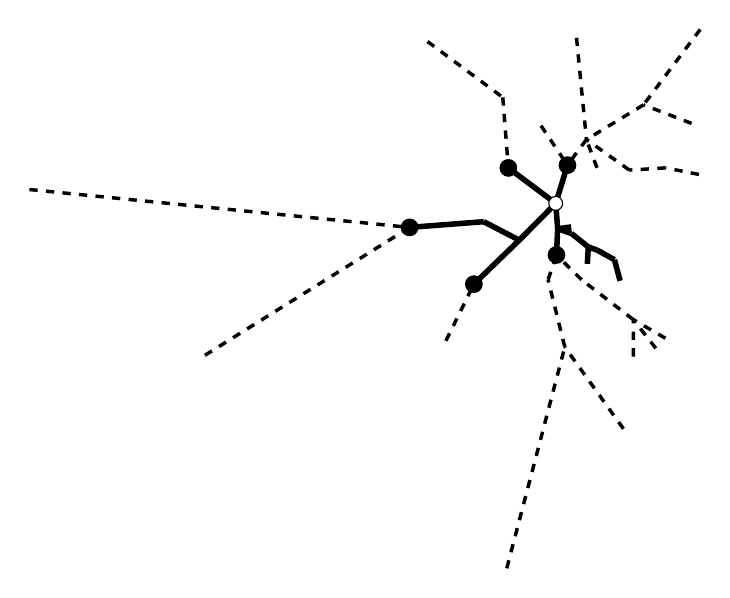
\begin{tikzpicture}[scale=1.5]
    \draw[line width=2] (4.456048319873318, 3.0900255391060227) edge (4.456048319873318, 3.0900255391060227);
    \draw[line width=2] (4.472612660101305, 2.8750437520344008) edge (4.456048319873318, 3.0900255391060227);
    \draw[line width=2] (4.587260603652865, 2.8905717642487616) edge (4.472612660101305, 2.8750437520344008);
    \draw[line width=2] (4.5889971877098645, 2.835738571829438) edge (4.472612660101305, 2.8750437520344008);
    \draw[line width=2] (4.555467757087328, 3.413754167559091) edge (4.456048319873318, 3.0900255391060227);
    \draw[line width=2] (4.46260040552211, 2.6534343050634845) edge (4.472612660101305, 2.8750437520344008);
    \draw[line width=2] (4.1474929335649335, 2.778701673953776) edge (4.456048319873318, 3.0900255391060227);
    \draw[line width=2] (4.05516128339265, 3.390271423153024) edge (4.456048319873318, 3.0900255391060227);
    \draw[line width=2] (4.731898018021141, 2.721123549710569) edge (4.5889971877098645, 2.835738571829438);
    \draw[line width=2] (4.808163001152366, 2.6938667891350576) edge (4.731898018021141, 2.721123549710569);
    \draw[line width=2] (4.7237357395051305, 2.577961439629206) edge (4.731898018021141, 2.721123549710569);
    \draw[line width=2] (4.9535573880579165, 2.6129010328780566) edge (4.808163001152366, 2.6938667891350576);
    \draw[line width=2] (3.846534022946102, 2.9349334463667276) edge (4.1474929335649335, 2.778701673953776);
    \draw[line width=2] (5.001135338416418, 2.434584433495246) edge (4.9535573880579165, 2.6129010328780566);
    \draw[line width=2] (3.7631245777735245, 2.4062629283591264) edge (4.1474929335649335, 2.778701673953776);
    \draw[line width=2] (3.2194560637723413, 2.886617108472933) edge (3.846534022946102, 2.9349334463667276);

    \draw[dashed,line width=1.25] (4.716279893465014, 3.6306879162957273) edge (4.555467757087328, 3.413754167559091);
    \draw[dashed,line width=1.25] (4.391620967473386, 2.443260777703671) edge (4.46260040552211, 2.6534343050634845);
    \draw[dashed,line width=1.25] (4.675476662781719, 2.4429315389880912) edge (4.46260040552211, 2.6534343050634845);
    \draw[dashed,line width=1.25] (4.331246054122673, 3.7480404128842792) edge (4.555467757087328, 3.413754167559091);
    \draw[dashed,line width=1.25] (4.805591520916153, 3.3906551281084774) edge (4.716279893465014, 3.6306879162957273);
    \draw[dashed,line width=1.25] (5.080161044919507, 3.3717017518306136) edge (4.716279893465014, 3.6306879162957273);
    \draw[dashed,line width=1.25] (4.007883808656132, 3.987747576108802) edge (4.05516128339265, 3.390271423153024);
    \draw[dashed,line width=1.25] (5.199329852951351, 3.9242600178816645) edge (4.716279893465014, 3.6306879162957273);
    \draw[dashed,line width=1.25] (4.5328890621807005, 1.8742850719746684) edge (4.391620967473386, 2.443260777703671);
    \draw[dashed,line width=1.25] (5.112877843259156, 2.1060471378532952) edge (4.675476662781719, 2.4429315389880912);
    \draw[dashed,line width=1.25] (5.385844366594839, 3.3906551281084774) edge (5.080161044919507, 3.3717017518306136);

    \draw[dashed,line width=1.25] (5.113512787335495, 1.7932534850537252) edge (5.112877843259156, 2.1060471378532952);
    \draw[dashed,line width=1.25] (5.3852877691412, 1.9481038374912885) edge (5.112877843259156, 2.1060471378532952);
    \draw[dashed,line width=1.25] (3.370595393721487, 4.4601669764603) edge (4.007883808656132, 3.987747576108802);
    \draw[dashed,line width=1.25] (5.029308443523917, 1.1816258114066613) edge (4.5328890621807005, 1.8742850719746684);
    \draw[dashed,line width=1.25] (3.5261803967035377, 1.9263597014372635) edge (3.7631245777735245, 2.4062629283591264);
    \draw[dashed,line width=1.25] (4.041647477097499, 0.0) edge (4.5328890621807005, 1.8742850719746684);
    \draw[dashed,line width=1.25] (0.0, 3.2073226303808156) edge (3.2194560637723413, 2.886617108472933);
    \draw[dashed,line width=1.25] (5.6063671485642175, 3.7671352248452195) edge (5.199329852951351, 3.9242600178816645);
    \draw[dashed,line width=1.25] (5.303556091896411, 1.8632888735496067) edge (5.112877843259156, 2.1060471378532952);
    \draw[dashed,line width=1.25] (5.679759184661748, 4.563044474936362) edge (5.199329852951351, 3.9242600178816645);
    \draw[dashed,line width=1.25] (5.668072671564062, 3.3352093179608744) edge (5.385844366594839, 3.3906551281084774);
    \draw[dashed,line width=1.25] (1.4858865913254249, 1.803766838849441) edge (3.2194560637723413, 2.886617108472933);
    \draw[dashed,line width=1.25] (4.6321645700874825, 4.491935662294821) edge (4.716279893465014, 3.6306879162957273);

    \filldraw (4.555467757087328, 3.413754167559091) circle (2pt);
    \filldraw (4.46260040552211, 2.6534343050634845) circle (2pt);
    \filldraw (4.05516128339265, 3.390271423153024) circle (2pt);
    \filldraw (3.7631245777735245, 2.4062629283591264) circle (2pt);
    \filldraw (3.2194560637723413, 2.886617108472933) circle (2pt);

    %\filldraw (4.456048319873318, 3.0900255391060227) circle (2pt);
    \node[circle,draw=black, fill=white, inner sep=0pt, minimum size=5pt] at (4.456048319873318, 3.0900255391060227) {};
  \end{tikzpicture}
  \caption{CH-PEOPLE Suchbaum auf aegaeis-graph}
  \label{fig:ergebnisse:ch_people_suchbaum}
\end{figure}

Nach der Untersuchung des einzelnen Suchvorganges wurden für aegaeis-graph für alle Knoten die bei der CH-PEOPLE-Suche gesehen Knoten erfasst.
Die Ergebnisse sind hierbei in \autoref{fig:ergebnisse:efficiency_ch_people} gelistet.
Bei \num{65}\% aller Suchen wurden weniger als \num{1}\% der \num{524881} Knoten gesehen.
Es ist anzunehmen, dass durch eine bessere vertex-to-level-Funktion noch mehr Suchen \emph{lokaler} werden.

\begin{figure}[h!]%
  \centering
  \begin{tikzpicture}
    \begin{axis}[
        tick align=outside,
        tick pos=left,
        x grid style={darkgray176},
        xlabel={Gesehene Knoten (\%)},
        xmin=-5, xmax=105,
        xtick style={color=black},
        xtick={-20,0,20,40,60,80,100,120},
        xticklabels={\ensuremath{-}20,0,20,40,60,80,100,120},
        y grid style={darkgray176},
        ylabel={Anteil aller Suchen (\%)},
        ymin=0, ymax=0.68283477588288,
        ytick style={color=black},
        ytick={0,0.1,0.2,0.3,0.4,0.5,0.6,0.7},
        yticklabels={0,10,20,30,40,50,60,70}
      ]
      \draw[pattern=north east lines, pattern color=CadetBlue] (axis cs:0,0) rectangle (axis cs:1,0.650318834174171);
      \draw[pattern=north east lines, pattern color=CadetBlue] (axis cs:1,0) rectangle (axis cs:2,0.0261163959069088);
      \draw[pattern=north east lines, pattern color=CadetBlue] (axis cs:2,0) rectangle (axis cs:3,0.0121417997603392);
      \draw[pattern=north east lines, pattern color=CadetBlue] (axis cs:3,0) rectangle (axis cs:4,0.00762458538221844);
      \draw[pattern=north east lines, pattern color=CadetBlue] (axis cs:4,0) rectangle (axis cs:5,0.00591943697714958);
      \draw[pattern=north east lines, pattern color=CadetBlue] (axis cs:5,0) rectangle (axis cs:6,0.00413808082213352);
      \draw[pattern=north east lines, pattern color=CadetBlue] (axis cs:6,0) rectangle (axis cs:7,0.0037684732348896);
      \draw[pattern=north east lines, pattern color=CadetBlue] (axis cs:7,0) rectangle (axis cs:8,0.00317214759155249);
      \draw[pattern=north east lines, pattern color=CadetBlue] (axis cs:8,0) rectangle (axis cs:9,0.00266346086065494);
      \draw[pattern=north east lines, pattern color=CadetBlue] (axis cs:9,0) rectangle (axis cs:10,0.00286922178551252);
      \draw[pattern=north east lines, pattern color=CadetBlue] (axis cs:10,0) rectangle (axis cs:11,0.00370179145368577);
      \draw[pattern=north east lines, pattern color=CadetBlue] (axis cs:11,0) rectangle (axis cs:12,0.00250914016701176);
      \draw[pattern=north east lines, pattern color=CadetBlue] (axis cs:12,0) rectangle (axis cs:13,0.00217954164849032);
      \draw[pattern=north east lines, pattern color=CadetBlue] (axis cs:13,0) rectangle (axis cs:14,0.0018994781674343);
      \draw[pattern=north east lines, pattern color=CadetBlue] (axis cs:14,0) rectangle (axis cs:15,0.0015108186427033);
      \draw[pattern=north east lines, pattern color=CadetBlue] (axis cs:15,0) rectangle (axis cs:16,0.00119455648042266);
      \draw[pattern=north east lines, pattern color=CadetBlue] (axis cs:16,0) rectangle (axis cs:17,0.00104785656177409);
      \draw[pattern=north east lines, pattern color=CadetBlue] (axis cs:17,0) rectangle (axis cs:18,0.00181374444874349);
      \draw[pattern=north east lines, pattern color=CadetBlue] (axis cs:18,0) rectangle (axis cs:19,0.0011621681866949);
      \draw[pattern=north east lines, pattern color=CadetBlue] (axis cs:19,0) rectangle (axis cs:20,0.000874483930644265);
      \draw[pattern=north east lines, pattern color=CadetBlue] (axis cs:20,0) rectangle (axis cs:21,0.00245007916080286);
      \draw[pattern=north east lines, pattern color=CadetBlue] (axis cs:21,0) rectangle (axis cs:22,0.00248246745453029);
      \draw[pattern=north east lines, pattern color=CadetBlue] (axis cs:22,0) rectangle (axis cs:23,0.00250151939201715);
      \draw[pattern=north east lines, pattern color=CadetBlue] (axis cs:23,0) rectangle (axis cs:24,0.00151843941769825);
      \draw[pattern=north east lines, pattern color=CadetBlue] (axis cs:24,0) rectangle (axis cs:25,0.000830664474424814);
      \draw[pattern=north east lines, pattern color=CadetBlue] (axis cs:25,0) rectangle (axis cs:26,0.00121551361165795);
      \draw[pattern=north east lines, pattern color=CadetBlue] (axis cs:26,0) rectangle (axis cs:27,0.00128981616785639);
      \draw[pattern=north east lines, pattern color=CadetBlue] (axis cs:27,0) rectangle (axis cs:28,0.00128219539286178);
      \draw[pattern=north east lines, pattern color=CadetBlue] (axis cs:28,0) rectangle (axis cs:29,0.0039894757097364);
      \draw[pattern=north east lines, pattern color=CadetBlue] (axis cs:29,0) rectangle (axis cs:30,0.00172229514880695);
      \draw[pattern=north east lines, pattern color=CadetBlue] (axis cs:30,0) rectangle (axis cs:31,0.00136792911155248);
      \draw[pattern=north east lines, pattern color=CadetBlue] (axis cs:31,0) rectangle (axis cs:32,0.00192615087991577);
      \draw[pattern=north east lines, pattern color=CadetBlue] (axis cs:32,0) rectangle (axis cs:33,0.00115454741170029);
      \draw[pattern=north east lines, pattern color=CadetBlue] (axis cs:33,0) rectangle (axis cs:34,0.00117740973668445);
      \draw[pattern=north east lines, pattern color=CadetBlue] (axis cs:34,0) rectangle (axis cs:35,0.00108215004925027);
      \draw[pattern=north east lines, pattern color=CadetBlue] (axis cs:35,0) rectangle (axis cs:36,0.000988795555565081);
      \draw[pattern=north east lines, pattern color=CadetBlue] (axis cs:36,0) rectangle (axis cs:37,0.00104023578677936);
      \draw[pattern=north east lines, pattern color=CadetBlue] (axis cs:37,0) rectangle (axis cs:38,0.000685869749524892);
      \draw[pattern=north east lines, pattern color=CadetBlue] (axis cs:38,0) rectangle (axis cs:39,0.00248056226078164);
      \draw[pattern=north east lines, pattern color=CadetBlue] (axis cs:39,0) rectangle (axis cs:40,0.00177373538002135);
      \draw[pattern=north east lines, pattern color=CadetBlue] (axis cs:40,0) rectangle (axis cs:41,0.00124409151788818);
      \draw[pattern=north east lines, pattern color=CadetBlue] (axis cs:41,0) rectangle (axis cs:42,0.00176992499252404);
      \draw[pattern=north east lines, pattern color=CadetBlue] (axis cs:42,0) rectangle (axis cs:43,0.000956407261837544);
      \draw[pattern=north east lines, pattern color=CadetBlue] (axis cs:43,0) rectangle (axis cs:44,0.00181564964249215);
      \draw[pattern=north east lines, pattern color=CadetBlue] (axis cs:44,0) rectangle (axis cs:45,0.00151653422394948);
      \draw[pattern=north east lines, pattern color=CadetBlue] (axis cs:45,0) rectangle (axis cs:46,0.00239292334834229);
      \draw[pattern=north east lines, pattern color=CadetBlue] (axis cs:46,0) rectangle (axis cs:47,0.00170324321132043);
      \draw[pattern=north east lines, pattern color=CadetBlue] (axis cs:47,0) rectangle (axis cs:48,0.00103642539928195);
      \draw[pattern=north east lines, pattern color=CadetBlue] (axis cs:48,0) rectangle (axis cs:49,0.00108215004925039);
      \draw[pattern=north east lines, pattern color=CadetBlue] (axis cs:49,0) rectangle (axis cs:50,0.00138698104903923);
      \draw[pattern=north east lines, pattern color=CadetBlue] (axis cs:50,0) rectangle (axis cs:51,0.000621093162069708);
      \draw[pattern=north east lines, pattern color=CadetBlue] (axis cs:51,0) rectangle (axis cs:52,0.00110882276173196);
      \draw[pattern=north east lines, pattern color=CadetBlue] (axis cs:52,0) rectangle (axis cs:53,0.00302925806040166);
      \draw[pattern=north east lines, pattern color=CadetBlue] (axis cs:53,0) rectangle (axis cs:54,0.00227861172342159);
      \draw[pattern=north east lines, pattern color=CadetBlue] (axis cs:54,0) rectangle (axis cs:55,0.00165561336760311);
      \draw[pattern=north east lines, pattern color=CadetBlue] (axis cs:55,0) rectangle (axis cs:56,0.00112025392422388);
      \draw[pattern=north east lines, pattern color=CadetBlue] (axis cs:56,0) rectangle (axis cs:57,0.00205951444232344);
      \draw[pattern=north east lines, pattern color=CadetBlue] (axis cs:57,0) rectangle (axis cs:58,0.00140793818027474);
      \draw[pattern=north east lines, pattern color=CadetBlue] (axis cs:58,0) rectangle (axis cs:59,0.000691585330770961);
      \draw[pattern=north east lines, pattern color=CadetBlue] (axis cs:59,0) rectangle (axis cs:60,0.00104214098052813);
      \draw[pattern=north east lines, pattern color=CadetBlue] (axis cs:60,0) rectangle (axis cs:61,0.00138698104903912);
      \draw[pattern=north east lines, pattern color=CadetBlue] (axis cs:61,0) rectangle (axis cs:62,0.000502971149651588);
      \draw[pattern=north east lines, pattern color=CadetBlue] (axis cs:62,0) rectangle (axis cs:63,0.00190138336118284);
      \draw[pattern=north east lines, pattern color=CadetBlue] (axis cs:63,0) rectangle (axis cs:64,0.00123266035539626);
      \draw[pattern=north east lines, pattern color=CadetBlue] (axis cs:64,0) rectangle (axis cs:65,0.00440480794694864);
      \draw[pattern=north east lines, pattern color=CadetBlue] (axis cs:65,0) rectangle (axis cs:66,0.00320834627277755);
      \draw[pattern=north east lines, pattern color=CadetBlue] (axis cs:66,0) rectangle (axis cs:67,0.00282159194179543);
      \draw[pattern=north east lines, pattern color=CadetBlue] (axis cs:67,0) rectangle (axis cs:68,0.00207094560481547);
      \draw[pattern=north east lines, pattern color=CadetBlue] (axis cs:68,0) rectangle (axis cs:69,0.00175087305503696);
      \draw[pattern=north east lines, pattern color=CadetBlue] (axis cs:69,0) rectangle (axis cs:70,0.00218144684223898);
      \draw[pattern=north east lines, pattern color=CadetBlue] (axis cs:70,0) rectangle (axis cs:71,0.00120789283666334);
      \draw[pattern=north east lines, pattern color=CadetBlue] (axis cs:71,0) rectangle (axis cs:72,0.00121170322416064);
      \draw[pattern=north east lines, pattern color=CadetBlue] (axis cs:72,0) rectangle (axis cs:73,0.00120598764291446);
      \draw[pattern=north east lines, pattern color=CadetBlue] (axis cs:73,0) rectangle (axis cs:74,0.00148414593022206);
      \draw[pattern=north east lines, pattern color=CadetBlue] (axis cs:74,0) rectangle (axis cs:75,0.000682059362027698);
      \draw[pattern=north east lines, pattern color=CadetBlue] (axis cs:75,0) rectangle (axis cs:76,0.0010040371055543);
      \draw[pattern=north east lines, pattern color=CadetBlue] (axis cs:76,0) rectangle (axis cs:77,0.00308831906661078);
      \draw[pattern=north east lines, pattern color=CadetBlue] (axis cs:77,0) rectangle (axis cs:78,0.00205379886107737);
      \draw[pattern=north east lines, pattern color=CadetBlue] (axis cs:78,0) rectangle (axis cs:79,0.00400090687222843);
      \draw[pattern=north east lines, pattern color=CadetBlue] (axis cs:79,0) rectangle (axis cs:80,0.00244436357955691);
      \draw[pattern=north east lines, pattern color=CadetBlue] (axis cs:80,0) rectangle (axis cs:81,0.00208809234855345);
      \draw[pattern=north east lines, pattern color=CadetBlue] (axis cs:81,0) rectangle (axis cs:82,0.00528119707134167);
      \draw[pattern=north east lines, pattern color=CadetBlue] (axis cs:82,0) rectangle (axis cs:83,0.00305402557913448);
      \draw[pattern=north east lines, pattern color=CadetBlue] (axis cs:83,0) rectangle (axis cs:84,0.00230528443590305);
      \draw[pattern=north east lines, pattern color=CadetBlue] (axis cs:84,0) rectangle (axis cs:85,0.00455341305934576);
      \draw[pattern=north east lines, pattern color=CadetBlue] (axis cs:85,0) rectangle (axis cs:86,0.00329217479771948);
      \draw[pattern=north east lines, pattern color=CadetBlue] (axis cs:86,0) rectangle (axis cs:87,0.00422953012207028);
      \draw[pattern=north east lines, pattern color=CadetBlue] (axis cs:87,0) rectangle (axis cs:88,0.00162322507387547);
      \draw[pattern=north east lines, pattern color=CadetBlue] (axis cs:88,0) rectangle (axis cs:89,0.00502590110901857);
      \draw[pattern=north east lines, pattern color=CadetBlue] (axis cs:89,0) rectangle (axis cs:90,0.00425239244705433);
      \draw[pattern=north east lines, pattern color=CadetBlue] (axis cs:90,0) rectangle (axis cs:91,0.00176039902378056);
      \draw[pattern=north east lines, pattern color=CadetBlue] (axis cs:91,0) rectangle (axis cs:92,0.00117169415543839);
      \draw[pattern=north east lines, pattern color=CadetBlue] (axis cs:92,0) rectangle (axis cs:93,0.00560698520236602);
      \draw[pattern=north east lines, pattern color=CadetBlue] (axis cs:93,0) rectangle (axis cs:94,0.00772746584464701);
      \draw[pattern=north east lines, pattern color=CadetBlue] (axis cs:94,0) rectangle (axis cs:95,0.00288255814175331);
      \draw[pattern=north east lines, pattern color=CadetBlue] (axis cs:95,0) rectangle (axis cs:96,0.00501446994652632);
      \draw[pattern=north east lines, pattern color=CadetBlue] (axis cs:96,0) rectangle (axis cs:97,0.0057098656647947);
      \draw[pattern=north east lines, pattern color=CadetBlue] (axis cs:97,0) rectangle (axis cs:98,0.00931639743104651);
      \draw[pattern=north east lines, pattern color=CadetBlue] (axis cs:98,0) rectangle (axis cs:99,0.0207113612419031);
      \draw[pattern=north east lines, pattern color=CadetBlue] (axis cs:99,0) rectangle (axis cs:100,0.0650433145799436);
    \end{axis}
  \end{tikzpicture}
  \caption{Anteil der pro CH-PEOPLE Suche auf aegaeis-graph gesehenen Knoten}
  \label{fig:ergebnisse:efficiency_ch_people}
\end{figure}

\subsection{Vergleich verschiedener vertex-to-level-Funktionen}


Wie im  \autoref{chapter:people} erwähnt, lässt sich die durch eine vertex-to-level-Funktion induzierte durchschnittliche Labelgröße vorhersagen, indem für $n \in \mathbb{N}$ zufällig ausgewählte Knoten die Labels berechnet und von diesen die durchschnittliche Labelgröße bestimmt wird.
Diese Methode wurde verwendet, um verschiedene Funktionen zu vergleichen, die Ergebnisse sind in \autoref{table:ergebnisse:vtl_vergleich} gelistet.

Es wurden sechs vertex-to-level-Funktionen verglichen. Drei davon basierten auf einem Hitting-Set über \num{1000000}, wobei Knoten, die nicht im Hitting-Set enthalten waren, nach einer weiteren Metrik sortiert wurden. Diese war entweder eine zufällige Sortierung, eine Sortierung nach Grad (aufsteigend nach Grad) oder eine Sortierung danach, auf wie vielen kürzesten Pfaden die Knoten liegen.

Die anderen drei Funktionen waren eine zufällige Sortierung, eine Sortierung nach Grad sowie die Übernahme der vertex-to-Level-Funktion, die durch die Graphen-Kontraktion der triangulierten Graphen entstand.
Letztere, in der Tabelle als $\triangle$ notiert, führte zu überraschend kleinen Labels.

\begin{table}[h!]
  \centering
  \begin{tabular}{l
      S[table-format = 6.0] % random
      S[table-format = 6.0] % random
      S[table-format = 6.0] % random
      S[table-format = 6.0] % random
      S[table-format = 6.0] % random
      S[table-format = 6.0] % random
    }
    \toprule
    Graph              & \multicolumn{3}{c}{Hitting-Set}   & {$\triangle$} & {Zufällig} & {Grad}   \\ \cline{2-4}
                       & {Zufällig} & {Hits}     & {Grad}  &               &            &          \\
    \midrule
    aegaeis-visibility & 1747.03    & \B 1420.17 & 1582.00 & 1473.27       & 17811.58   & 7420.85  \\
    medi-visibility    & 2487.06    & 2002.87    & 2422.12 & \B 1930.65    & 18700.13   & 12862.80 \\
    pata-visibility    & 1100.42    & \B 478.80  & 806.95  & 552.90        & 23690.52   & 10174.37 \\
    \bottomrule
  \end{tabular}
  \caption{Vorhergesagt durchschnittliche Labelgröße für verschiedene vertex-to-level-Funktion}
  \label{table:ergebnisse:vtl_vergleich}
\end{table}

\subsection{Große Hitting-Sets}

Mit den erzeugten Hub-Graphen wurden jeweils Hitting-Sets über \num{250000000} Pfade gebildet.
Die Knoten, die nicht enthalten waren, wurden danach sortiert, wie oft sie auf kürzesten Pfaden lagen, da dies nach \autoref{table:ergebnisse:vtl_vergleich} erfolgversprechend erscheint.
Mit dieser vertex-to-level-Funktion wurde über \num{10000} Labels die durchschnittliche Labelgröße vorhergesagt, die Ergebnisse sind in \autoref{fig:ergebnisse:250_paths} aufgelistet.
Für die Sichtbarkeitsgraphen von aegaeis und medi ist die durchschnittliche Labelgröße kleiner als der ursprüngliche durchschnittliche Knotengrad.

\begin{table}[h!]
  \centering
  \begin{tabular}{ %VERGLEICH
      l % Graph
      r
      S[table-format = 4.1] % average time
    }
    \toprule
    {Graph}            & {Erstellung} & {$\varnothing$ $\abs{\text{Label}}$} \\ \midrule
    aegaeis-graph      & 6h 12m       & 90.8                                 \\
    aegaeis-visibility & 8h 11m       & 1309.8                               \\
    medi-graph         & 4h 47m       & 88.5                                 \\
    medi-visibility    & 12h 26m      & 1739.4                               \\
    pata-graph         & 2d 10h 37m   & 99.3                                 \\
    pata-visibility    & 9h 29m       & 424.1                                \\  \bottomrule
  \end{tabular}
  \caption{Vorhergesagt durchschnittliche Labelgröße für vertex-to-level-Funktionen über jeweils \num{250000000} Pfade}
  \label{fig:ergebnisse:250_paths}
\end{table}

Mit der entstandenen vertex-to-level-Funktion für aegaeis-graph wurde das der \autoref{fig:ergebnisse:efficiency_ch_people} zugrunde liegende Experiment wiederholt, wobei diesmal \num{86.7}\% aller Suchen weniger als 1\% aller Knoten sahen.
\autoref{fig:ergebnisse:new_efficiency_ch_people} zeigt die Abbildung mit den neuen Daten.

\begin{figure}
  \centering
  \begin{tikzpicture}
    \begin{axis}[
        tick align=outside,
        tick pos=left,
        x grid style={darkgray176},
        xlabel={Gesehene Knoten (\%)},
        xmin=-5, xmax=105,
        xtick style={color=black},
        xtick={-20,0,20,40,60,80,100,120},
        xticklabels={\ensuremath{-}20,0,20,40,60,80,100,120},
        y grid style={darkgray176},
        ylabel={Anteil aller Suchen (\%)},
        ymin=0, ymax=0.910038275342993,
        ytick style={color=black},
        ytick={0,0.1,0.2,0.3,0.4,0.5,0.6,0.7,0.8},
        yticklabels={0,10,20,30,40,50,60,70,80}
      ]
      \draw[pattern=north east lines, pattern color=CadetBlue] (axis cs:0,0) rectangle (axis cs:1,0.866703119374279);
      \draw[pattern=north east lines, pattern color=CadetBlue] (axis cs:1,0) rectangle (axis cs:2,0.0200159655236347);
      \draw[pattern=north east lines, pattern color=CadetBlue] (axis cs:2,0) rectangle (axis cs:3,0.00872769256270434);
      \draw[pattern=north east lines, pattern color=CadetBlue] (axis cs:3,0) rectangle (axis cs:4,0.00569271892105661);
      \draw[pattern=north east lines, pattern color=CadetBlue] (axis cs:4,0) rectangle (axis cs:5,0.00354556556629393);
      \draw[pattern=north east lines, pattern color=CadetBlue] (axis cs:5,0) rectangle (axis cs:6,0.00217382606724403);
      \draw[pattern=north east lines, pattern color=CadetBlue] (axis cs:6,0) rectangle (axis cs:7,0.00153939654893376);
      \draw[pattern=north east lines, pattern color=CadetBlue] (axis cs:7,0) rectangle (axis cs:8,0.00157369003640984);
      \draw[pattern=north east lines, pattern color=CadetBlue] (axis cs:8,0) rectangle (axis cs:9,0.00189185739243969);
      \draw[pattern=north east lines, pattern color=CadetBlue] (axis cs:9,0) rectangle (axis cs:10,0.00180421848000012);
      \draw[pattern=north east lines, pattern color=CadetBlue] (axis cs:10,0) rectangle (axis cs:11,0.00173372631129898);
      \draw[pattern=north east lines, pattern color=CadetBlue] (axis cs:11,0) rectangle (axis cs:12,0.00117359934918704);
      \draw[pattern=north east lines, pattern color=CadetBlue] (axis cs:12,0) rectangle (axis cs:13,0.000939260518099339);
      \draw[pattern=north east lines, pattern color=CadetBlue] (axis cs:13,0) rectangle (axis cs:14,0.00104785656177431);
      \draw[pattern=north east lines, pattern color=CadetBlue] (axis cs:14,0) rectangle (axis cs:15,0.0013622135303063);
      \draw[pattern=north east lines, pattern color=CadetBlue] (axis cs:15,0) rectangle (axis cs:16,0.00103452020553341);
      \draw[pattern=north east lines, pattern color=CadetBlue] (axis cs:16,0) rectangle (axis cs:17,0.00116026299294614);
      \draw[pattern=north east lines, pattern color=CadetBlue] (axis cs:17,0) rectangle (axis cs:18,0.000956407261837655);
      \draw[pattern=north east lines, pattern color=CadetBlue] (axis cs:18,0) rectangle (axis cs:19,0.00076779308071806);
      \draw[pattern=north east lines, pattern color=CadetBlue] (axis cs:19,0) rectangle (axis cs:20,0.000855431993157407);
      \draw[pattern=north east lines, pattern color=CadetBlue] (axis cs:20,0) rectangle (axis cs:21,0.000737309980739287);
      \draw[pattern=north east lines, pattern color=CadetBlue] (axis cs:21,0) rectangle (axis cs:22,0.00110691756798331);
      \draw[pattern=north east lines, pattern color=CadetBlue] (axis cs:22,0) rectangle (axis cs:23,0.000672533393284103);
      \draw[pattern=north east lines, pattern color=CadetBlue] (axis cs:23,0) rectangle (axis cs:24,0.000544885412122498);
      \draw[pattern=north east lines, pattern color=CadetBlue] (axis cs:24,0) rectangle (axis cs:25,0.00051821269964103);
      \draw[pattern=north east lines, pattern color=CadetBlue] (axis cs:25,0) rectangle (axis cs:26,0.000615377580823528);
      \draw[pattern=north east lines, pattern color=CadetBlue] (axis cs:26,0) rectangle (axis cs:27,0.000802086568194471);
      \draw[pattern=north east lines, pattern color=CadetBlue] (axis cs:27,0) rectangle (axis cs:28,0.000603946418331835);
      \draw[pattern=north east lines, pattern color=CadetBlue] (axis cs:28,0) rectangle (axis cs:29,0.000977364393072833);
      \draw[pattern=north east lines, pattern color=CadetBlue] (axis cs:29,0) rectangle (axis cs:30,0.00054679060587115);
      \draw[pattern=north east lines, pattern color=CadetBlue] (axis cs:30,0) rectangle (axis cs:31,0.000417237430961115);
      \draw[pattern=north east lines, pattern color=CadetBlue] (axis cs:31,0) rectangle (axis cs:32,0.000918303386863828);
      \draw[pattern=north east lines, pattern color=CadetBlue] (axis cs:32,0) rectangle (axis cs:33,0.00080780214944054);
      \draw[pattern=north east lines, pattern color=CadetBlue] (axis cs:33,0) rectangle (axis cs:34,0.000621093162069708);
      \draw[pattern=north east lines, pattern color=CadetBlue] (axis cs:34,0) rectangle (axis cs:35,0.000703016493262987);
      \draw[pattern=north east lines, pattern color=CadetBlue] (axis cs:35,0) rectangle (axis cs:36,0.000459151693431914);
      \draw[pattern=north east lines, pattern color=CadetBlue] (axis cs:36,0) rectangle (axis cs:37,0.000994511136811038);
      \draw[pattern=north east lines, pattern color=CadetBlue] (axis cs:37,0) rectangle (axis cs:38,0.000455341305934609);
      \draw[pattern=north east lines, pattern color=CadetBlue] (axis cs:38,0) rectangle (axis cs:39,0.000497255568405519);
      \draw[pattern=north east lines, pattern color=CadetBlue] (axis cs:39,0) rectangle (axis cs:40,0.000302925806040188);
      \draw[pattern=north east lines, pattern color=CadetBlue] (axis cs:40,0) rectangle (axis cs:41,0.000424858205955725);
      \draw[pattern=north east lines, pattern color=CadetBlue] (axis cs:41,0) rectangle (axis cs:42,0.000360081618500541);
      \draw[pattern=north east lines, pattern color=CadetBlue] (axis cs:42,0) rectangle (axis cs:43,0.000245769993579836);
      \draw[pattern=north east lines, pattern color=CadetBlue] (axis cs:43,0) rectangle (axis cs:44,0.000470582855924051);
      \draw[pattern=north east lines, pattern color=CadetBlue] (axis cs:44,0) rectangle (axis cs:45,0.000716352849503665);
      \draw[pattern=north east lines, pattern color=CadetBlue] (axis cs:45,0) rectangle (axis cs:46,0.000605851612080377);
      \draw[pattern=north east lines, pattern color=CadetBlue] (axis cs:46,0) rectangle (axis cs:47,0.000426763399704266);
      \draw[pattern=north east lines, pattern color=CadetBlue] (axis cs:47,0) rectangle (axis cs:48,0.000394375105976841);
      \draw[pattern=north east lines, pattern color=CadetBlue] (axis cs:48,0) rectangle (axis cs:49,0.000169562243632626);
      \draw[pattern=north east lines, pattern color=CadetBlue] (axis cs:49,0) rectangle (axis cs:50,0.000316262162280867);
      \draw[pattern=north east lines, pattern color=CadetBlue] (axis cs:50,0) rectangle (axis cs:51,0.000251485574825683);
      \draw[pattern=north east lines, pattern color=CadetBlue] (axis cs:51,0) rectangle (axis cs:52,0.000417237430961115);
      \draw[pattern=north east lines, pattern color=CadetBlue] (axis cs:52,0) rectangle (axis cs:53,0.000983079974318901);
      \draw[pattern=north east lines, pattern color=CadetBlue] (axis cs:53,0) rectangle (axis cs:54,0.000659197037043535);
      \draw[pattern=north east lines, pattern color=CadetBlue] (axis cs:54,0) rectangle (axis cs:55,0.000565842543357897);
      \draw[pattern=north east lines, pattern color=CadetBlue] (axis cs:55,0) rectangle (axis cs:56,0.000706826880760403);
      \draw[pattern=north east lines, pattern color=CadetBlue] (axis cs:56,0) rectangle (axis cs:57,0.000744930755734008);
      \draw[pattern=north east lines, pattern color=CadetBlue] (axis cs:57,0) rectangle (axis cs:58,0.000699206105765682);
      \draw[pattern=north east lines, pattern color=CadetBlue] (axis cs:58,0) rectangle (axis cs:59,0.000413427043463588);
      \draw[pattern=north east lines, pattern color=CadetBlue] (axis cs:59,0) rectangle (axis cs:60,0.000783034630707502);
      \draw[pattern=north east lines, pattern color=CadetBlue] (axis cs:60,0) rectangle (axis cs:61,0.00049725556840563);
      \draw[pattern=north east lines, pattern color=CadetBlue] (axis cs:61,0) rectangle (axis cs:62,0.00021528689360073);
      \draw[pattern=north east lines, pattern color=CadetBlue] (axis cs:62,0) rectangle (axis cs:63,0.00050297114965181);
      \draw[pattern=north east lines, pattern color=CadetBlue] (axis cs:63,0) rectangle (axis cs:64,0.00043628936844764);
      \draw[pattern=north east lines, pattern color=CadetBlue] (axis cs:64,0) rectangle (axis cs:65,0.000683964555776351);
      \draw[pattern=north east lines, pattern color=CadetBlue] (axis cs:65,0) rectangle (axis cs:66,0.000558221768363176);
      \draw[pattern=north east lines, pattern color=CadetBlue] (axis cs:66,0) rectangle (axis cs:67,0.000525833474635751);
      \draw[pattern=north east lines, pattern color=CadetBlue] (axis cs:67,0) rectangle (axis cs:68,0.000525833474635862);
      \draw[pattern=north east lines, pattern color=CadetBlue] (axis cs:68,0) rectangle (axis cs:69,0.000424858205955614);
      \draw[pattern=north east lines, pattern color=CadetBlue] (axis cs:69,0) rectangle (axis cs:70,0.00056012696211194);
      \draw[pattern=north east lines, pattern color=CadetBlue] (axis cs:70,0) rectangle (axis cs:71,0.000527738668384403);
      \draw[pattern=north east lines, pattern color=CadetBlue] (axis cs:71,0) rectangle (axis cs:72,0.000908777418120565);
      \draw[pattern=north east lines, pattern color=CadetBlue] (axis cs:72,0) rectangle (axis cs:73,0.000430573787201793);
      \draw[pattern=north east lines, pattern color=CadetBlue] (axis cs:73,0) rectangle (axis cs:74,0.0011412110554595);
      \draw[pattern=north east lines, pattern color=CadetBlue] (axis cs:74,0) rectangle (axis cs:75,0.00102689943053857);
      \draw[pattern=north east lines, pattern color=CadetBlue] (axis cs:75,0) rectangle (axis cs:76,0.000708732074509166);
      \draw[pattern=north east lines, pattern color=CadetBlue] (axis cs:76,0) rectangle (axis cs:77,0.000866863155649544);
      \draw[pattern=north east lines, pattern color=CadetBlue] (axis cs:77,0) rectangle (axis cs:78,0.000748741143231313);
      \draw[pattern=north east lines, pattern color=CadetBlue] (axis cs:78,0) rectangle (axis cs:79,0.000760172305723228);
      \draw[pattern=north east lines, pattern color=CadetBlue] (axis cs:79,0) rectangle (axis cs:80,0.00082875928067605);
      \draw[pattern=north east lines, pattern color=CadetBlue] (axis cs:80,0) rectangle (axis cs:81,0.000931639743104618);
      \draw[pattern=north east lines, pattern color=CadetBlue] (axis cs:81,0) rectangle (axis cs:82,0.00129362655535381);
      \draw[pattern=north east lines, pattern color=CadetBlue] (axis cs:82,0) rectangle (axis cs:83,0.000443910143442583);
      \draw[pattern=north east lines, pattern color=CadetBlue] (axis cs:83,0) rectangle (axis cs:84,0.000575368512101382);
      \draw[pattern=north east lines, pattern color=CadetBlue] (axis cs:84,0) rectangle (axis cs:85,0.000882104705638986);
      \draw[pattern=north east lines, pattern color=CadetBlue] (axis cs:85,0) rectangle (axis cs:86,0.000363892005997957);
      \draw[pattern=north east lines, pattern color=CadetBlue] (axis cs:86,0) rectangle (axis cs:87,0.00102689943053869);
      \draw[pattern=north east lines, pattern color=CadetBlue] (axis cs:87,0) rectangle (axis cs:88,0.000887820286884944);
      \draw[pattern=north east lines, pattern color=CadetBlue] (axis cs:88,0) rectangle (axis cs:89,0.00134697198031675);
      \draw[pattern=north east lines, pattern color=CadetBlue] (axis cs:89,0) rectangle (axis cs:90,0.00190709894242913);
      \draw[pattern=north east lines, pattern color=CadetBlue] (axis cs:90,0) rectangle (axis cs:91,0.000531549055881708);
      \draw[pattern=north east lines, pattern color=CadetBlue] (axis cs:91,0) rectangle (axis cs:92,0.000274347899810068);
      \draw[pattern=north east lines, pattern color=CadetBlue] (axis cs:92,0) rectangle (axis cs:93,0.00159083678014793);
      \draw[pattern=north east lines, pattern color=CadetBlue] (axis cs:93,0) rectangle (axis cs:94,0.000556316574614635);
      \draw[pattern=north east lines, pattern color=CadetBlue] (axis cs:94,0) rectangle (axis cs:95,0.000318167356029742);
      \draw[pattern=north east lines, pattern color=CadetBlue] (axis cs:95,0) rectangle (axis cs:96,0.000998321524308343);
      \draw[pattern=north east lines, pattern color=CadetBlue] (axis cs:96,0) rectangle (axis cs:97,0.00191090932992632);
      \draw[pattern=north east lines, pattern color=CadetBlue] (axis cs:97,0) rectangle (axis cs:98,0.00277586729182711);
      \draw[pattern=north east lines, pattern color=CadetBlue] (axis cs:98,0) rectangle (axis cs:99,0.0051059192464632);
      \draw[pattern=north east lines, pattern color=CadetBlue] (axis cs:99,0) rectangle (axis cs:100,0.015043409839579);
    \end{axis}
  \end{tikzpicture}
  \caption{Anteil der pro CH-PEOPLE Suche auf aegaeis-graph gesehenen Knoten}
  \label{fig:ergebnisse:new_efficiency_ch_people}
\end{figure}

\subsection{Weiterer Graph}

Als letzter Teil dieser Arbeit wurde mit \emph{planet-shrunk-visibility} ein Sichtbarkeitsgraph betrachtet, der analog zu den Sichtbarkeitsgraphen von aegaeis, medi und pata konstruiert wurde, aber die gesamte Welt umfasst.
Er bestand aus \num{188030} Knoten und \num{173385124} Kanten.
Mittels PEOPLE konnte für ihn ein Hub-Graph erstellt werden, mit dem ein Speedup \num[round-mode=places,round-precision=0]{\fpeval{(529.377185*1000)/6.756}} im Vergleich zur Dijkstra-Suche erzielt wurde.

% \autoref{table:input_graphs_planet-shrunk-visibility} listet die Anzahl der Kanten und Knoten dieses Graphs auf.
% 
% \begin{table}[h!]
%   \centering
%   \begin{tabular}{
%       l % Graph
%       S[table-format = 7.0] % Zeit
%       S[table-format = 9.0] % Zeit
%       S[table-format = 4.1] % Zeit
%     }
%     \toprule
%     {Graph}                  & {\# Knoten} & {\# Kanten} & {$\varnothing$ Grad}      \\ \midrule
%     planet-shrunk-visibility & 188030      & 173385124   & \fpeval{173385124/188030} \\\bottomrule
%   \end{tabular}
%   \caption{Bearbeite Graphen}
%   \label{table:input_graphs_planet-shrunk-visibility}
% \end{table}
% 
% 
% \begin{table}[h!]
%   \centering
%   \begin{tabular}{
%       l % Graph
%       S[table-format = 4.1] % Zeit
%       S[table-format = 3.0] % hop-länge
%       S[table-format = 7.0] % rank
%       S[table-format = 7.0] % queue pops
%     }
%     \toprule
%     {Graph}                  & {$\varnothing$ $t({spd})$} & {$\varnothing$  Hop-Länge} & {$\varnothing$ Dijkstra-Rank} & {$\varnothing$ Queue-Pops} \\
%                              & {(\si{\ms})}               &                            &                               &                            \\
%     \midrule
%     planet-shrunk-visibility & 529.377185                 & 22.3786                    & 95053.74                      & 691017.2                   \\
%     \bottomrule
%   \end{tabular}
%   \caption{Kennwerte der Dijkstra-Suchen}
%   \label{fig:ergebnisse:dijkstra_planet-shrunk-visibility}
% \end{table}
% 
% 
% Running `target/release/investigate_hl -h tests/data/planet-shrunk-vis-fixed-hl.bincode -n 10000000`
% average label size 1154.5453757379141
% shortcuts 63174890
% getting random paths distances takes 6.756µs on average
% getting random paths takes 11.242µs on average

% Is graph bidirectional? true
% non trivial vertices: 188030
% trivial: 188030
% average degree is 922.1135
% sum of squared degree 422505182196
% Values over 10000 parallel searches
% average path hops len 22.3786
% average dijkstra_rank 95053.74
% average queue pops 691017.2
% 2xDijsktra per node for all nodes would take 14810.959127085s
% Value over 100 sequential searches
% Average dijkstra duration for path creation is 573.84923ms
% Average dijkstra duration for path distance is 529.377185ms
\chapter{Ausblick}

Mit der Kontraktion durch eine obere Schranke wurde eine Methode gefunden, welche die Top-Down Graphen-Kontraktion von Graphen mit hohen durchschnittlichen Knotengraden beschleunigen kann.
Es hat sich jedoch gezeigt, dass die erzielte Beschleunigung für die bearbeiteten Sichtbarkeitsgraphen nicht groß genug war, um die Kontraktion in angemessener Zeit zu ermöglichen.
In weiteren Arbeiten kann die Bedeutung dieser Methode untersucht und andere Kontraktions-Reihenfolgen betrachtet werden, die eine effizientere Kontraktion ermöglichen.

Mit CH-PEOPLE und PEOPLE wurden Methoden gefunden, mit denen zu den bearbeiteten Sichtbarkeitsgraphen Contracted- und Hub-Graphen erstellt werden können.
Wenngleich die Erstellung dieser rechenintensiv ist, so können diese dafür genutzt werden, um weitere Analysen zu ermöglichen, die bisher aufgrund der langen Dijkstra-Laufzeit nicht möglich waren, etwa um den Fehler nicht-optimaler Pfadfindungs-Algorithmen wie von Funke et al. \cite{funkescalable} zu bestimmen.
In einem weiteren Schritt können diese Methoden auch auf andere Graphen und Graphklassen angewendet werden.
Durch die mögliche Parallelisierung können auch größere Graphen bearbeitet werden, für die es bisher keine vergleichbar schnellen Speedup-Techniken gab.

Die Tatsache, dass die meisten CH-PEOPLE Suchen nur einen kleinen Teil aller Knoten sehen, könnte die teilweise Neuberechnung eines Contracted-Graphen nach der Änderung von Kantengewichten ermöglichen.
Es ist zu vermuten, dass dies insbesondere auf Straßengraphen effizient sein könnte.


\backmatter
\chapter*{Danksagung}


Der Autor dankt dem Land Baden-Württemberg für die Unterstützung durch bwHPC.

Der Autor den Probe- und Korrekturlesern Lily, Tobias
\printbibliography

\cleardoublepage
\thispagestyle{empty}
\pagenumbering{gobble}
\chapter*{Erklärung}

Ich versichere, diese Arbeit selbstständig verfasst zu haben.
Ich habe keine anderen als die angegebenen Quellen benutzt und alle wörtlich oder sinngemäß aus anderen Werken übernommene Aussagen als solche gekennzeichnet.
Weder diese Arbeit noch wesentliche Teile daraus waren bisher Gegenstand eines anderen Prüfungsverfahrens.
Ich habe diese Arbeit bisher weder teilweise noch vollständig veröffentlicht. Das elektronische Exemplar stimmt mit allen eingereichten Druck-Exemplaren überein.

\vspace{1cm}

\begin{flushright}
    8. Oktober 2024\hspace{0.5cm} \makebox[4cm]{\hrulefill}
\end{flushright}

\end{document}